\documentclass[10pt]{beamer}
\usepackage[english]{babel}
\usepackage[utf8]{inputenc}
\usepackage[T1]{fontenc}
\usepackage{helvet}
\usepackage{lipsum}  
\usepackage{graphicx,subfigure}
\usepackage{epstopdf}
%-------------------------------------------------------
% INFORMATION IN THE TITLE PAGE
%-------------------------------------------------------

\newcommand{\cstitle}{\textbf{Detección \textit{in Silico} de Neoantígenos Utilizando Transformers y Transfer Learning en el Marco de Desarrollo de Vacunas Personalizadas para Tratar el Cáncer}
\subtitle[]{Tésis de doctorado}}
\newcommand{\cscourseCode}{Detección de Neoantígenos}
\newcommand{\csauthor}{MSc. Vicente Machaca Arceda}
\institute[UNSA]{Universidad Nacional de San Agustín}
\newcommand{\csemail}{vmachaca@utec.edu.pe}
\newcommand{\instituteabr}{UTEC}
\newcommand{\nameUp}{}
\date{2023}
\title[\cscourseCode]{\cstitle}
\author{\csauthor}
%%%%%%%%%%%%%%%%%

%-------------------------------------------------------
% CHOOSE THE THEME
%-------------------------------------------------------
\def\mycmd{0} % UNSA
\def\mycmd{1} % SALLE
%\def\mycmd{2} % UTEC
%-------------------------------------------------------

\if\mycmd0
\usepackage{csformat}
\newcommand{\chref}[3][blue]{\href{#2}{\color{#1}{#3}}}%

\fi

\if\mycmd1
\usetheme[]{Feather}
\newcommand{\chref}[2]{	\href{#1}{{\usebeamercolor[bg]{Feather}#2}} }
\fi

\if\mycmd2
\usetheme{UTEC2020}	
\newcommand{\chref}[3][blue]{\href{#2}{\color{#1}{#3}}}%
\fi

\newcommand{\1}{
	\setbeamertemplate{background}{
		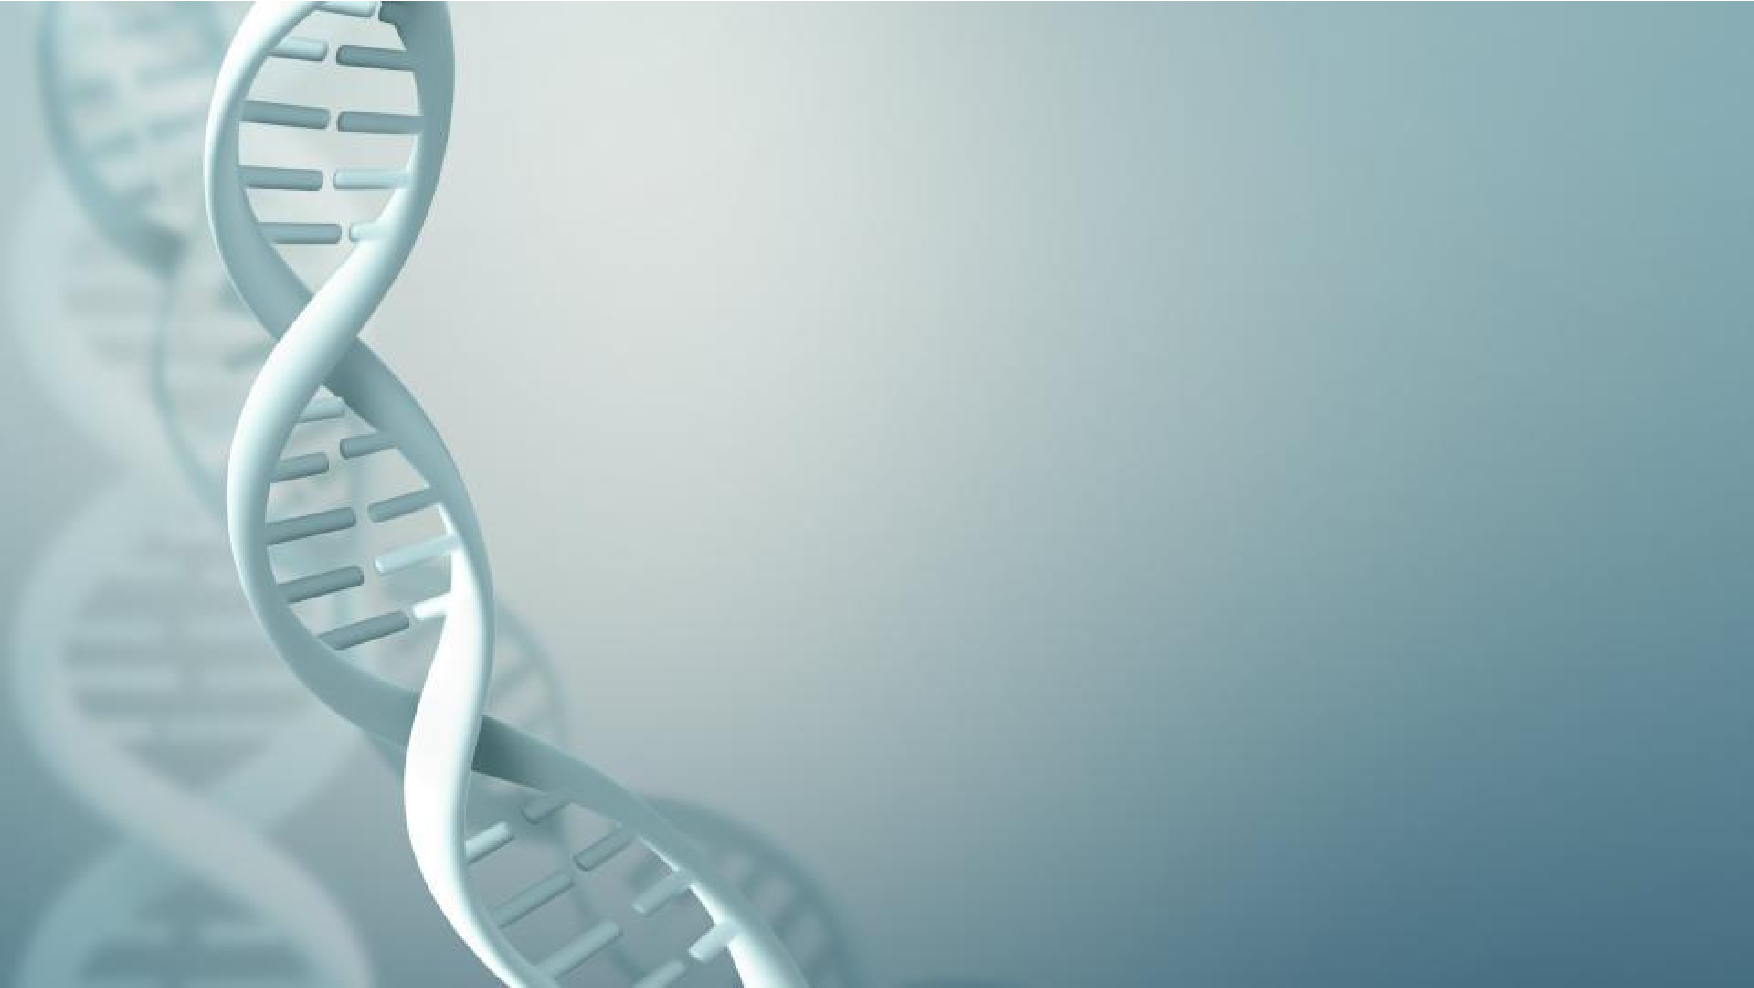
\includegraphics[width=\paperwidth,height=\paperheight]{img/1}
		\tikz[overlay] \fill[fill opacity=0.75,fill=white] (0,0) rectangle (-\paperwidth,\paperheight);
	}
}



%-------------------------------------------------------
% THE BODY OF THE PRESENTATION
%-------------------------------------------------------

\begin{document}
	
	
	\AtBeginSection[]
	{
		\begin{frame}
			\frametitle{Contenido}
			\tableofcontents[currentsection]
		\end{frame}
	}
	
	
	%-------------------------------------------------------
	% THE TITLEPAGE
	%-------------------------------------------------------
	
	\if\mycmd0
	\maketitle
	\fi
	
	\if\mycmd1 % MY THEME
	\1{
		\begin{frame}[plain,noframenumbering] 
			\titlepage 
	\end{frame}}
	\fi
	
	\if\mycmd2
	\begin{frame}
		\titlepage
	\end{frame}
	\fi
	%-------------------------------------------------------
	%-------------------------------------------------------


%-------------------------------------------------------
%-------------------------------------------------------
\begin{frame}{Contenido}
	\tableofcontents
\end{frame}
%-------------------------------------------------------
%-------------------------------------------------------


%%%%%%%%%%%%%%%%%%%%%%%%%%%%%%%%%%%%%%%%%%%%%%%%%%%%%%%%%%%%%%%%%%%%%%%%%%%%%%%%%%%%%%%%%%%%%%%%%%%%%%%%%%%%%%%%
%%%%%%%%%%%%%%%%%%%%%%%%%%%%%%%%%%%%%%%%%%%%%%%%%%%%%%%%%%%%%%%%%%%%%%%%%%%%%%%%%%%%%%%%%%%%%%%%%%%%%%%%%%%%%%%%
%%%%%%%%%%%%%%%%%%%%%%%%%%%%%%%%%%%%%%%%%%%%%%%%%%%%%%%%%%%%%%%%%%%%%%%%%%%%%%%%%%%%%%%%%%%%%%%%%%%%%%%%%%%%%%%%
\section{Contexto y Motivación}
%%%%%%%%%%%%%%%%%%%%%%%%%%%%%%%%%%%%%%%%%%%%%%%%%%%%%%%%%%%%%%%%%%%%%%%%%%%%%%%%%%%%%%%%%%%%%%%%%%%%%%%%%%%%%%%%
%%%%%%%%%%%%%%%%%%%%%%%%%%%%%%%%%%%%%%%%%%%%%%%%%%%%%%%%%%%%%%%%%%%%%%%%%%%%%%%%%%%%%%%%%%%%%%%%%%%%%%%%%%%%%%%%
%%%%%%%%%%%%%%%%%%%%%%%%%%%%%%%%%%%%%%%%%%%%%%%%%%%%%%%%%%%%%%%%%%%%%%%%%%%%%%%%%%%%%%%%%%%%%%%%%%%%%%%%%%%%%%%%

%%%%%%%%%%%%%%%%%%%%%%%%%%%%%%%%%%%%%%%%%%%%%%%%%%%%%%%%%%%%%%%%%%%%%%%%%%%%%%%%%%%%%%%%%%%%%%%%%%%%%%%%%%%%%%%%
\subsection{Estadísticas en Cáncer}
%%%%%%%%%%%%%%%%%%%%%%%%%%%%%%%%%%%%%%%%%%%%%%%%%%%%%%%%%%%%%%%%%%%%%%%%%%%%%%%%%%%%%%%%%%%%%%%%%%%%%%%%%%%%%%%%


%-------------------------------------------------------
%-------------------------------------------------------
%\begin{frame}{Contexto y Motivación}{}
%	\begin{block}{}
%		An la actualidad, el cáncer representa el mayor problema de salud mundial \cite{siegel2023cancer}.
%	\end{block}

	%\begin{figure}[]
	%	\centering
	%	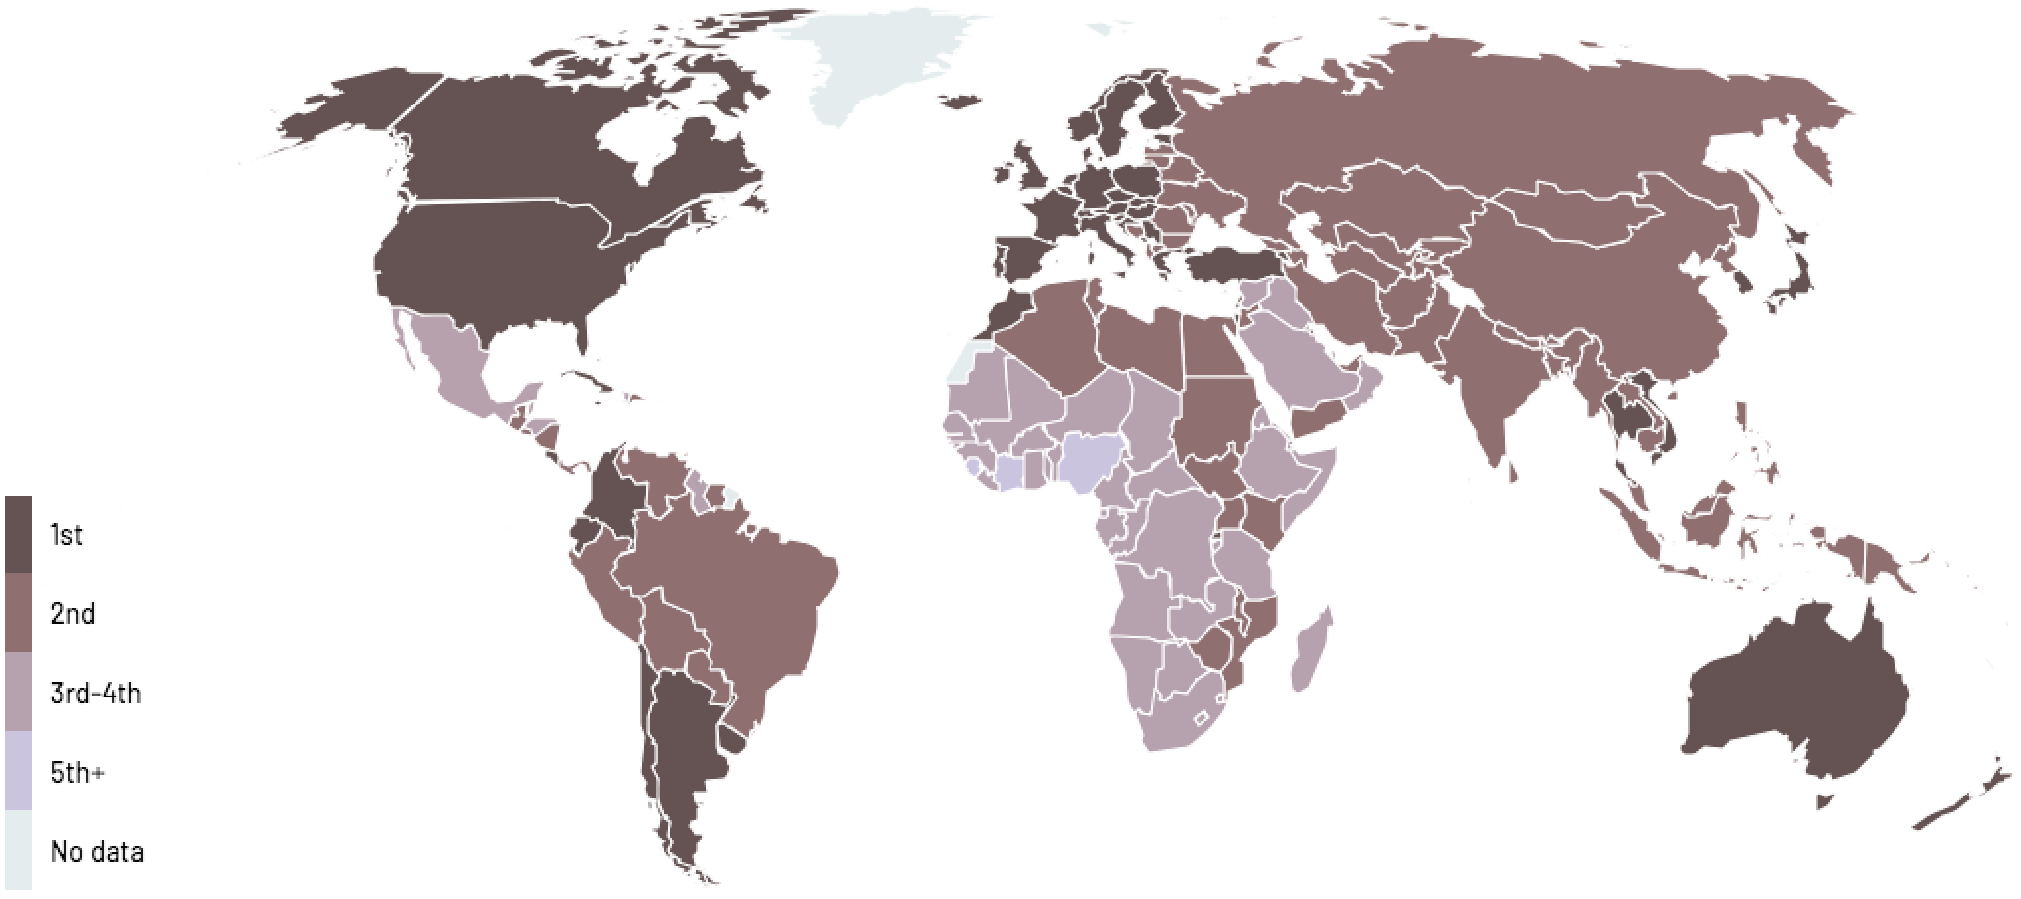
\includegraphics[width=\textwidth]{../img/introduction/cancer_deaths}
	%	\caption{Ranking de las muertes por cáncer entre 30 y 69 años. \textbf{Fuente}: Atlas Cancer \cite{canceratlas2023}.}
	%\end{figure}
%\end{frame}
%-------------------------------------------------------
%-------------------------------------------------------

%-------------------------------------------------------
%-------------------------------------------------------
%\begin{frame}{Contexto y Motivación}{Muertes por tipos de cáncer}
%	\begin{figure}[]
%		\centering
%		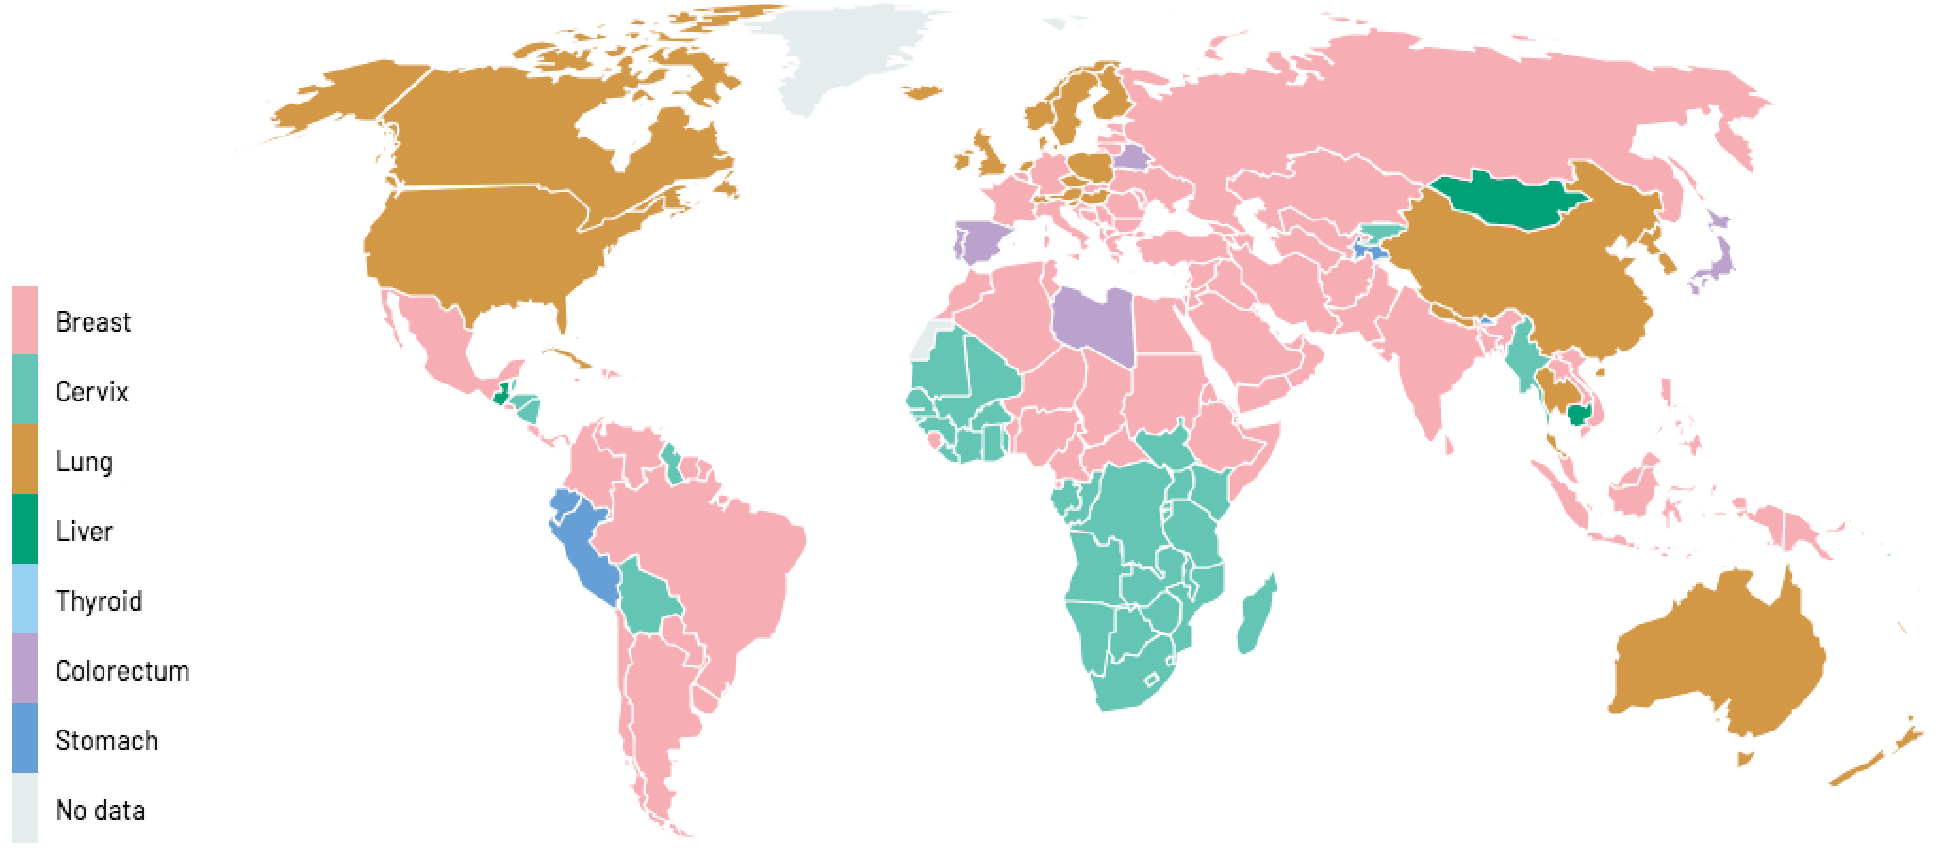
\includegraphics[width=\textwidth]{../img/introduction/cancer_deaths_woman}
%		\caption{Ranking de las muertes por tipo de cáncer en mujeres. \textbf{Fuente}: The Atlas Cancer \%cite{canceratlas2023}.}
%	\end{figure}
%\end{frame}
%-------------------------------------------------------
%-------------------------------------------------------


%-------------------------------------------------------
%-------------------------------------------------------
%\begin{frame}{Contexto y Motivación}{Muertes por tipos de cáncer}
%	\begin{figure}[]
%		\centering
%		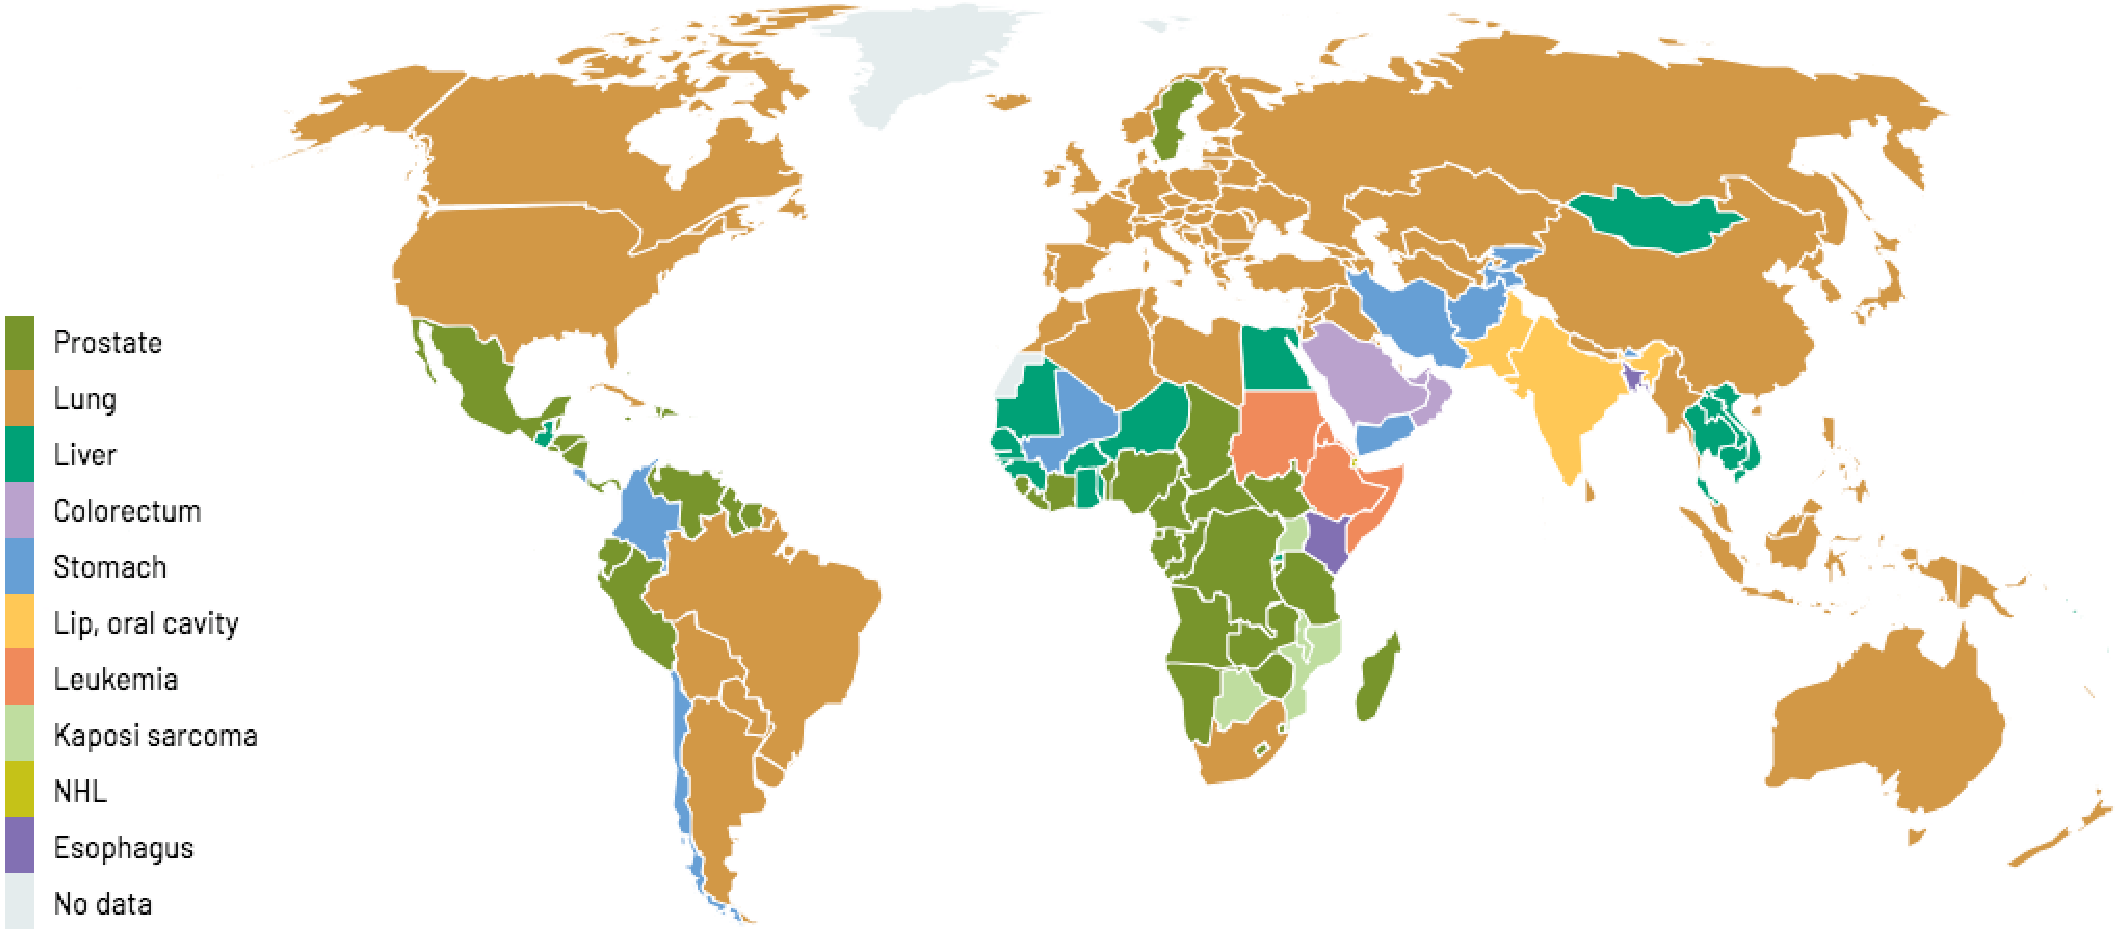
\includegraphics[width=\textwidth]{../img/introduction/cancer_deaths_man}
%		\caption{Ranking de las muertes por tipo de cáncer en hombres. \textbf{Fuente}: The Atlas Cancer \cite{canceratlas2023}.}
%	\end{figure}
%\end{frame}
%-------------------------------------------------------
%-------------------------------------------------------


%-------------------------------------------------------
%-------------------------------------------------------
\begin{frame}{Contexto y Motivación}{Porcentaje de casos y muertes}
	\begin{figure}[]
		\centering
		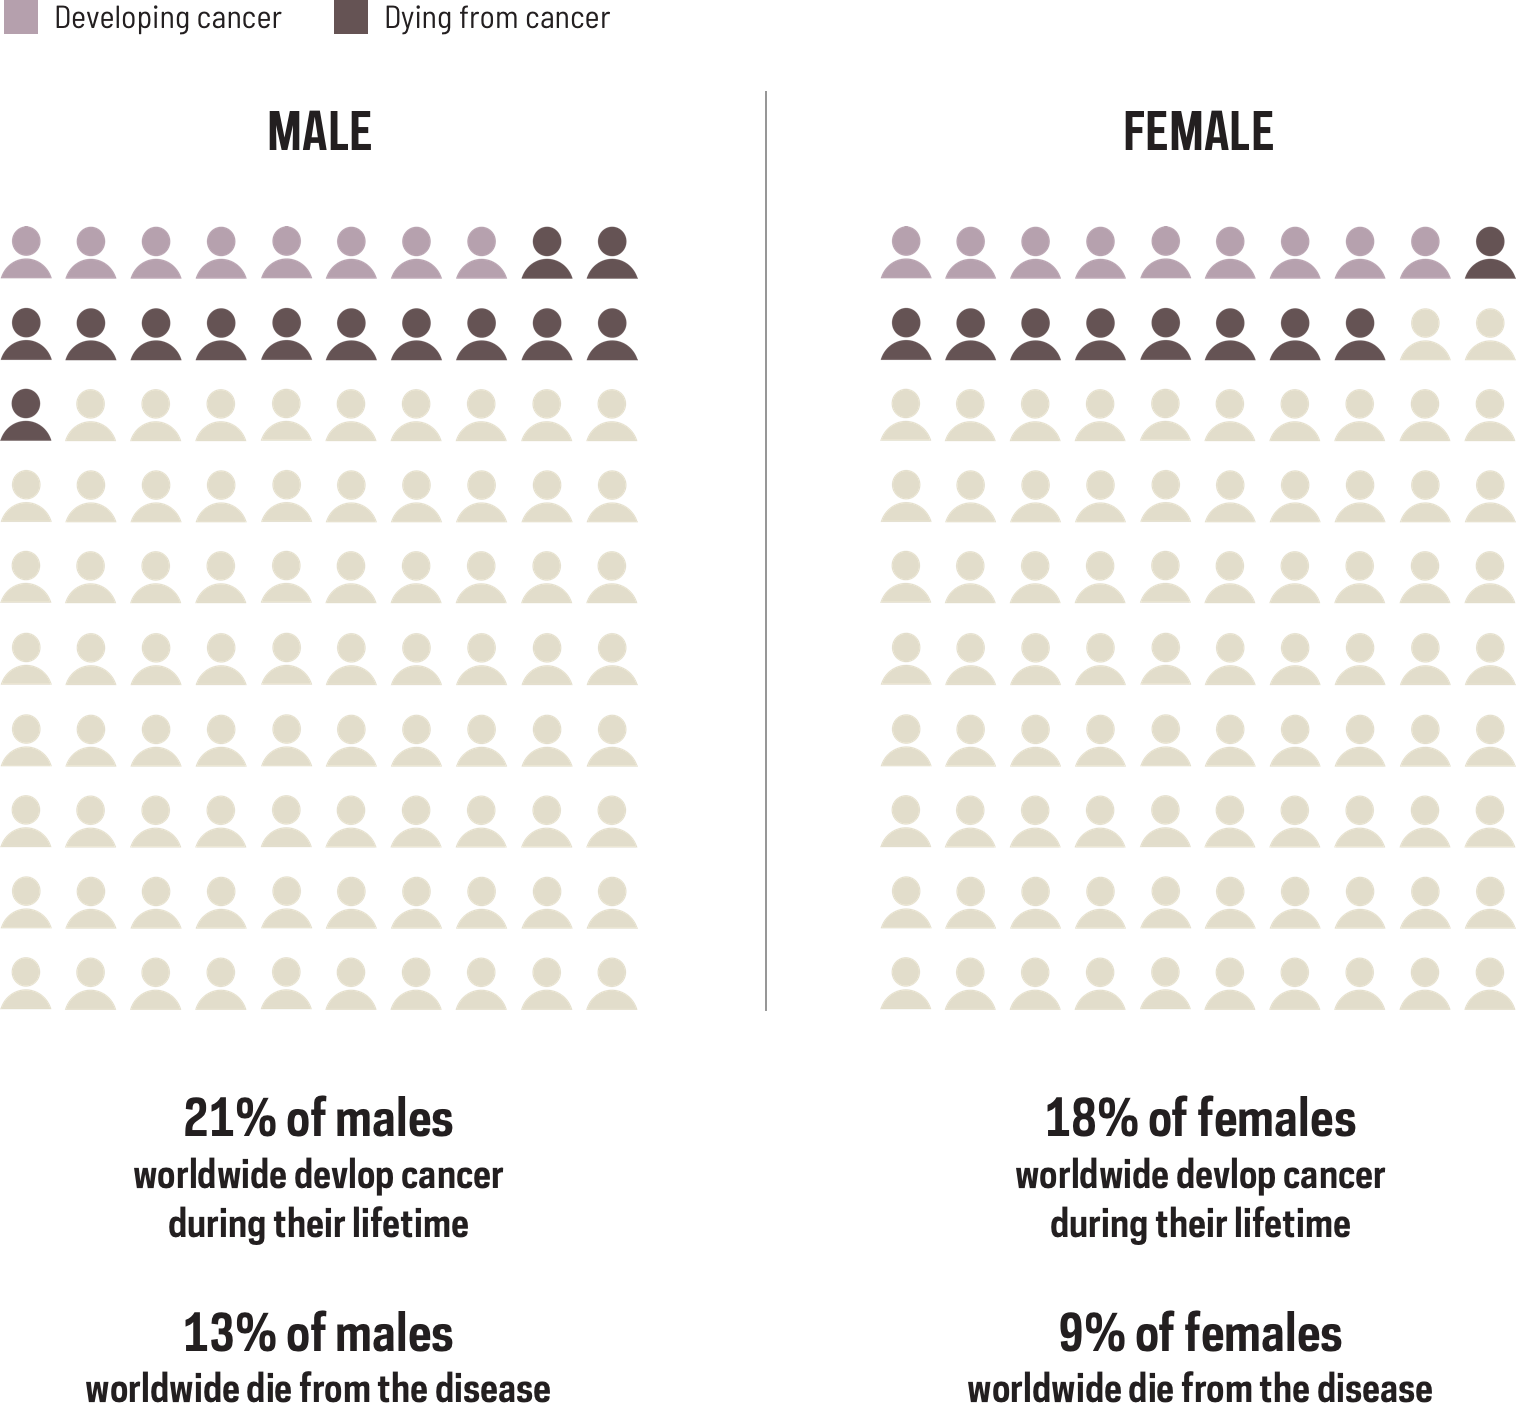
\includegraphics[width=0.6\textwidth]{../img/introduction/cancer_men_women}
		\caption{Porcentaje de casos y muertes por sexo. \textbf{Fuente} Atlas Cancer \cite{canceratlas2023}.}
	\end{figure}
\end{frame}
%-------------------------------------------------------
%-------------------------------------------------------

%-------------------------------------------------------
%-------------------------------------------------------
\begin{frame}{Contexto y Motivación}{Predicción de nuevos casos}
	\begin{figure}[]
		\centering
		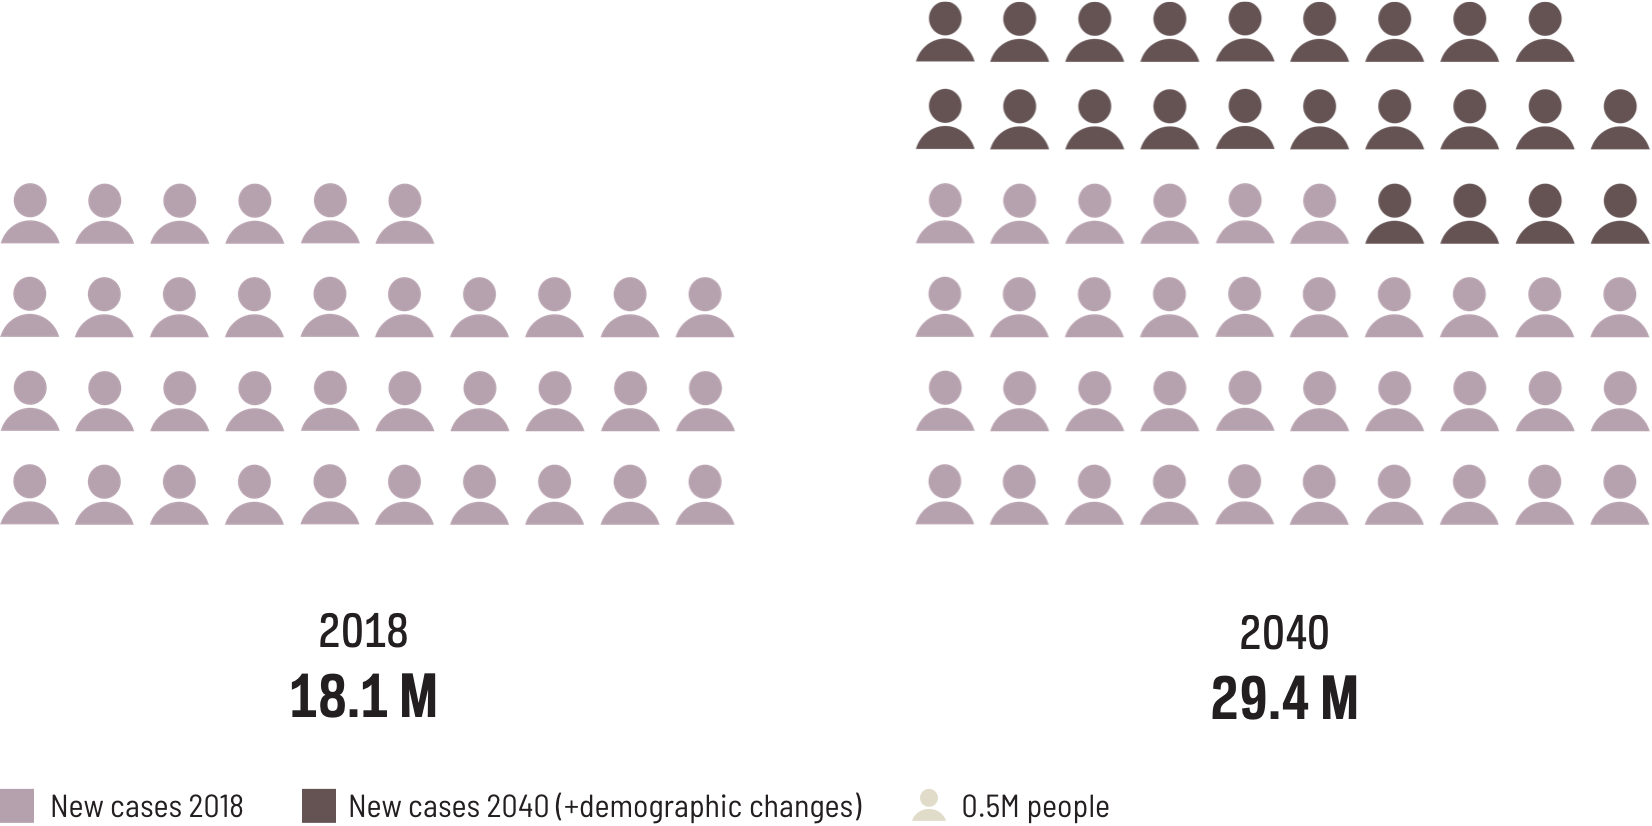
\includegraphics[width=\textwidth]{../img/introduction/cancer_new_cases}
		\caption{Predicción de nuevos casos para el 2040. \textbf{Fuente} Atlas Cancer \cite{canceratlas2023}.}
	\end{figure}
\end{frame}
%-------------------------------------------------------
%-------------------------------------------------------

%%%%%%%%%%%%%%%%%%%%%%%%%%%%%%%%%%%%%%%%%%%%%%%%%%%%%%%%%%%%%%%%%%%%%%%%%%%%%%%%%%%%%%%%%%%%%%%%%%%%%%%%%%%%%%%%
\subsection{Inmunoterapia del Cáncer}
%%%%%%%%%%%%%%%%%%%%%%%%%%%%%%%%%%%%%%%%%%%%%%%%%%%%%%%%%%%%%%%%%%%%%%%%%%%%%%%%%%%%%%%%%%%%%%%%%%%%%%%%%%%%%%%%



%-------------------------------------------------------
%-------------------------------------------------------
%\begin{frame}{Contexto y Motivación}{Reacciones distintas para cada paciente}

%	\begin{figure}[]
%		\centering
%		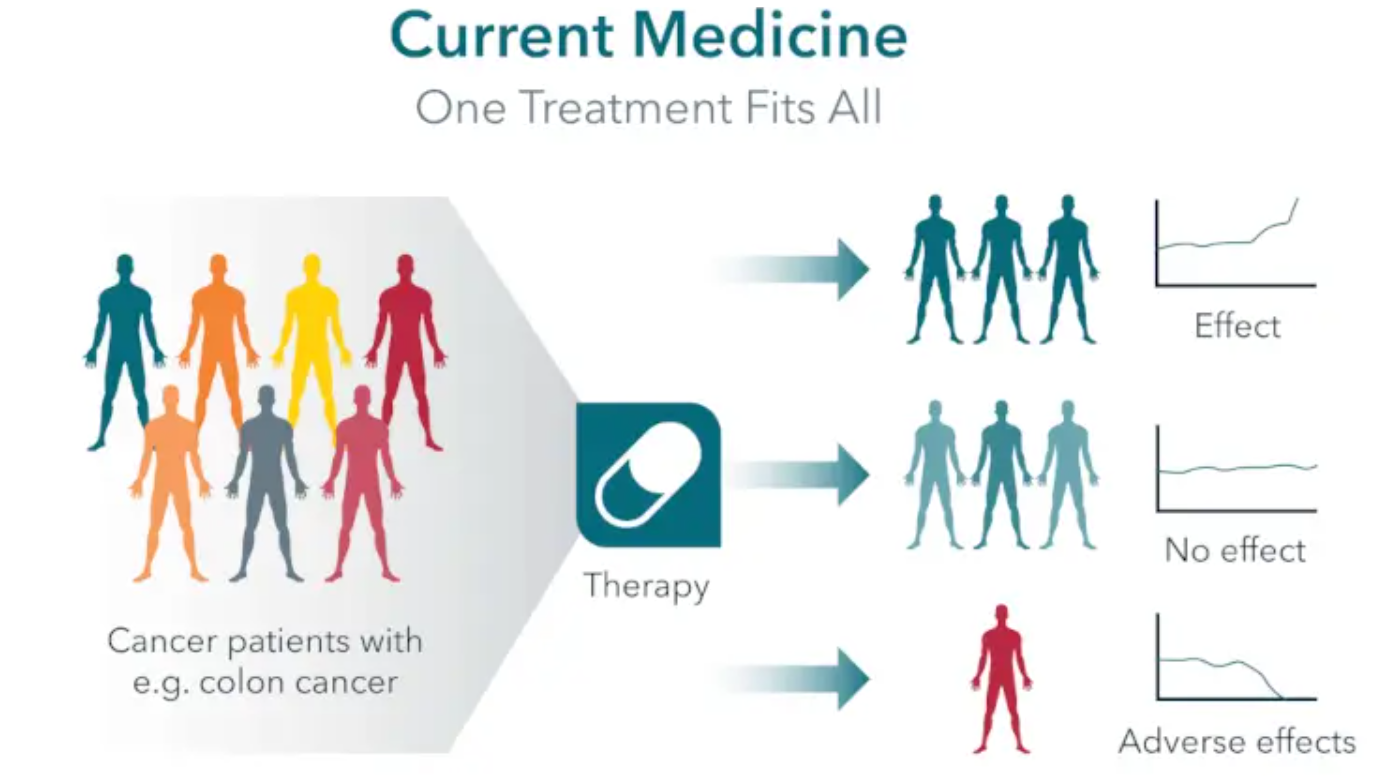
\includegraphics[width=\textwidth]{../img/introduction/medecine_current}
%			\caption{Pacientes con el mismo tipo de cáncer pueden reaccionar de forma disitinta a los mismos tratamientos. \textbf{Fuente} The Atlas Cancer \cite{pdx2023}.}
%	\end{figure}
%\end{frame}
%-------------------------------------------------------
%-------------------------------------------------------

%-------------------------------------------------------
%-------------------------------------------------------
%\begin{frame}{Contexto y Motivación}{Reacciones distintas para cada paciente}
	
%	\begin{figure}[]
%		\centering
%		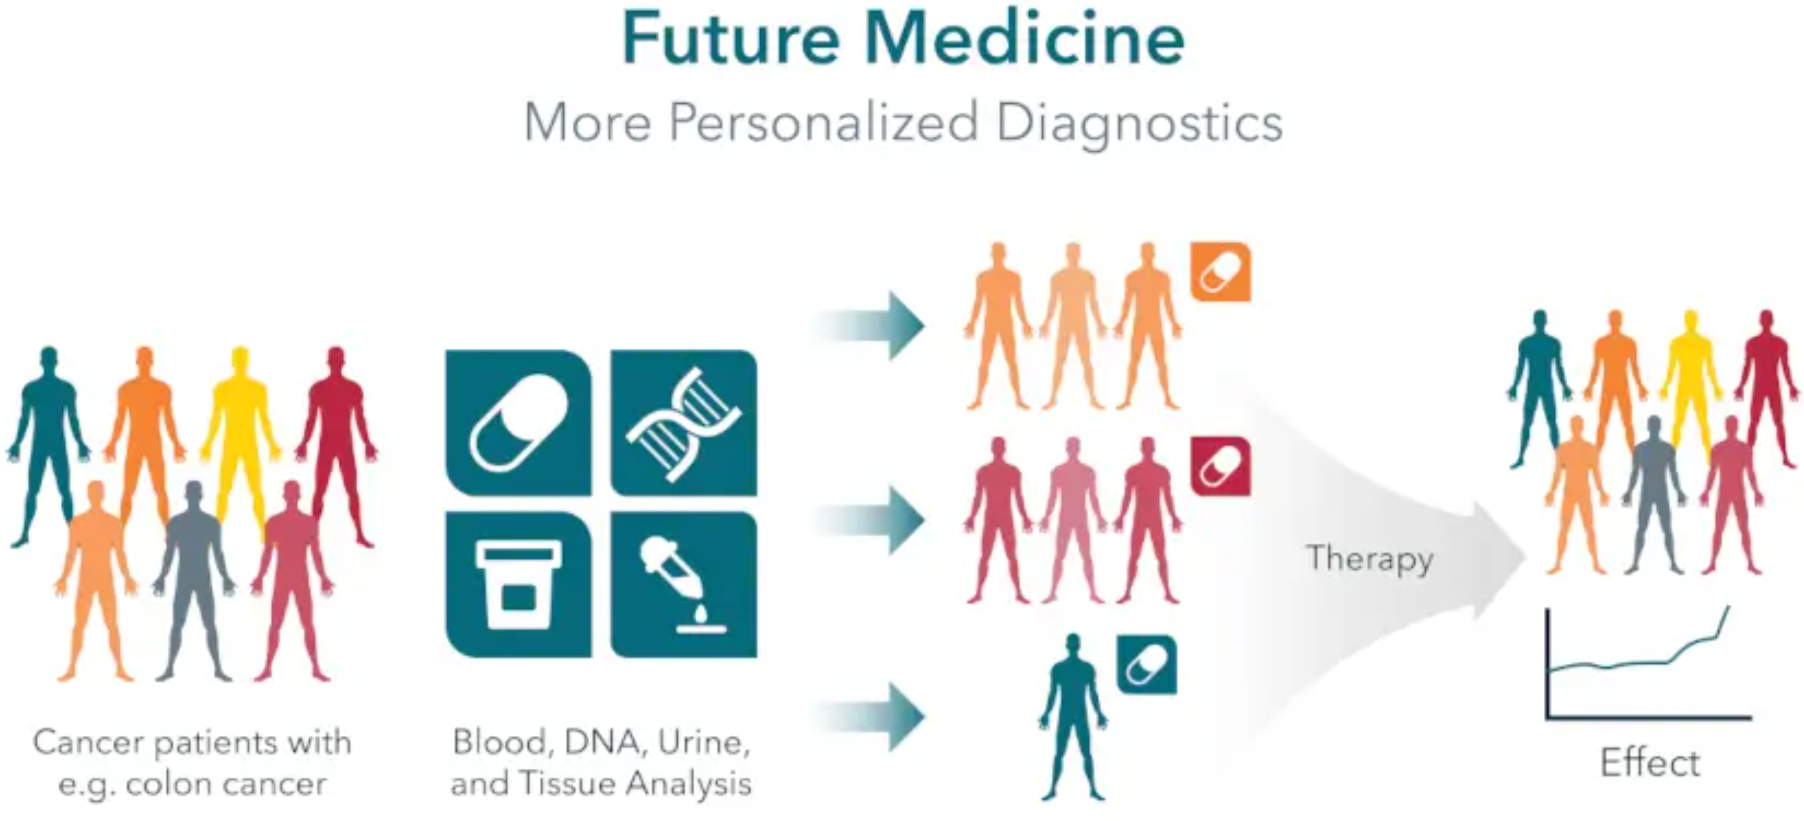
\includegraphics[width=\textwidth]{../img/introduction/medecine_future}
%		\caption{Cada paciente necesita un tratamiento personalizado. \textbf{Fuente} The Atlas Cancer \cite{pdx2023}.}
%	\end{figure}
%\end{frame}
%-------------------------------------------------------
%-------------------------------------------------------












%-------------------------------------------------------
%-------------------------------------------------------
%\begin{frame}{Inmunoterapia del Cáncer}{}		
%	Es un tipo de tratamiento contra el Cáncer que estimula las defensas naturales del cuerpo para combatir el Cáncer \cite{inmunoterapy2022}.
		
%	\begin{figure}
%		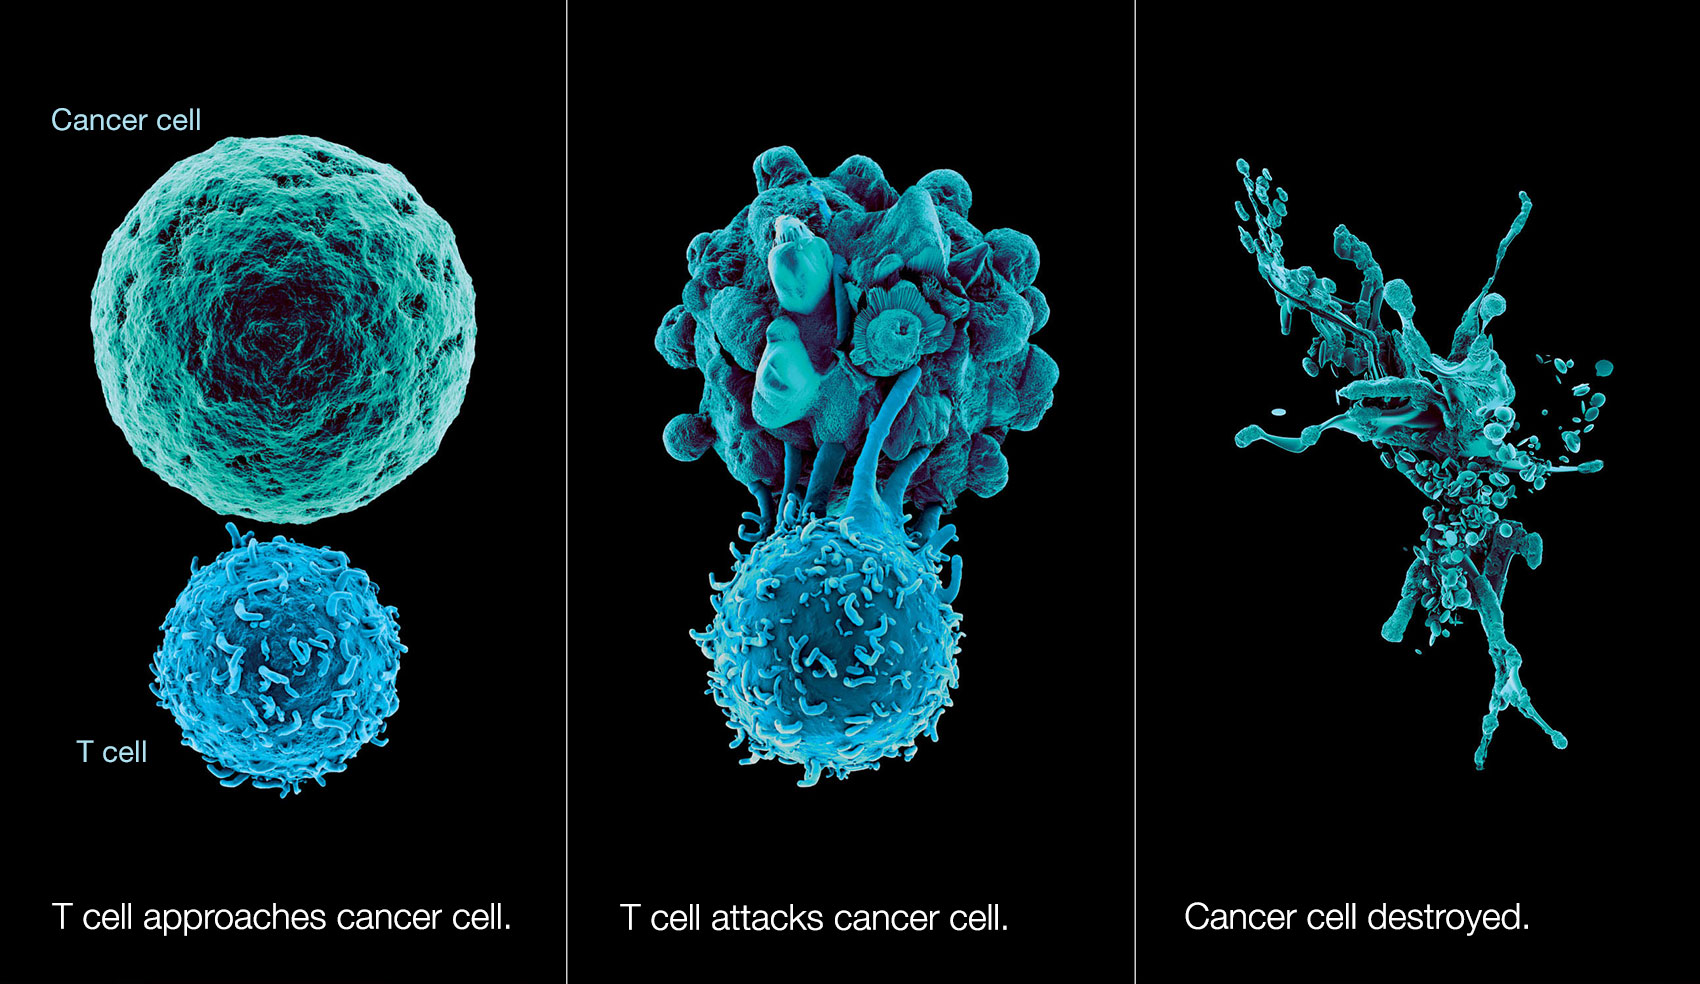
\includegraphics[width=0.85\textwidth]{../img/neoantigen/tcell}
%		\caption{Ejemplo de como una célula T destruye células del cancer \cite{nortshore2022}.}
%	\end{figure}		
%\end{frame}
%-------------------------------------------------------
%-------------------------------------------------------


%-------------------------------------------------------
%-------------------------------------------------------
\begin{frame}{Contexto y Motivación}{Inmunoterapia del Cáncer}
	
	
	\begin{figure}[]
		\centering
		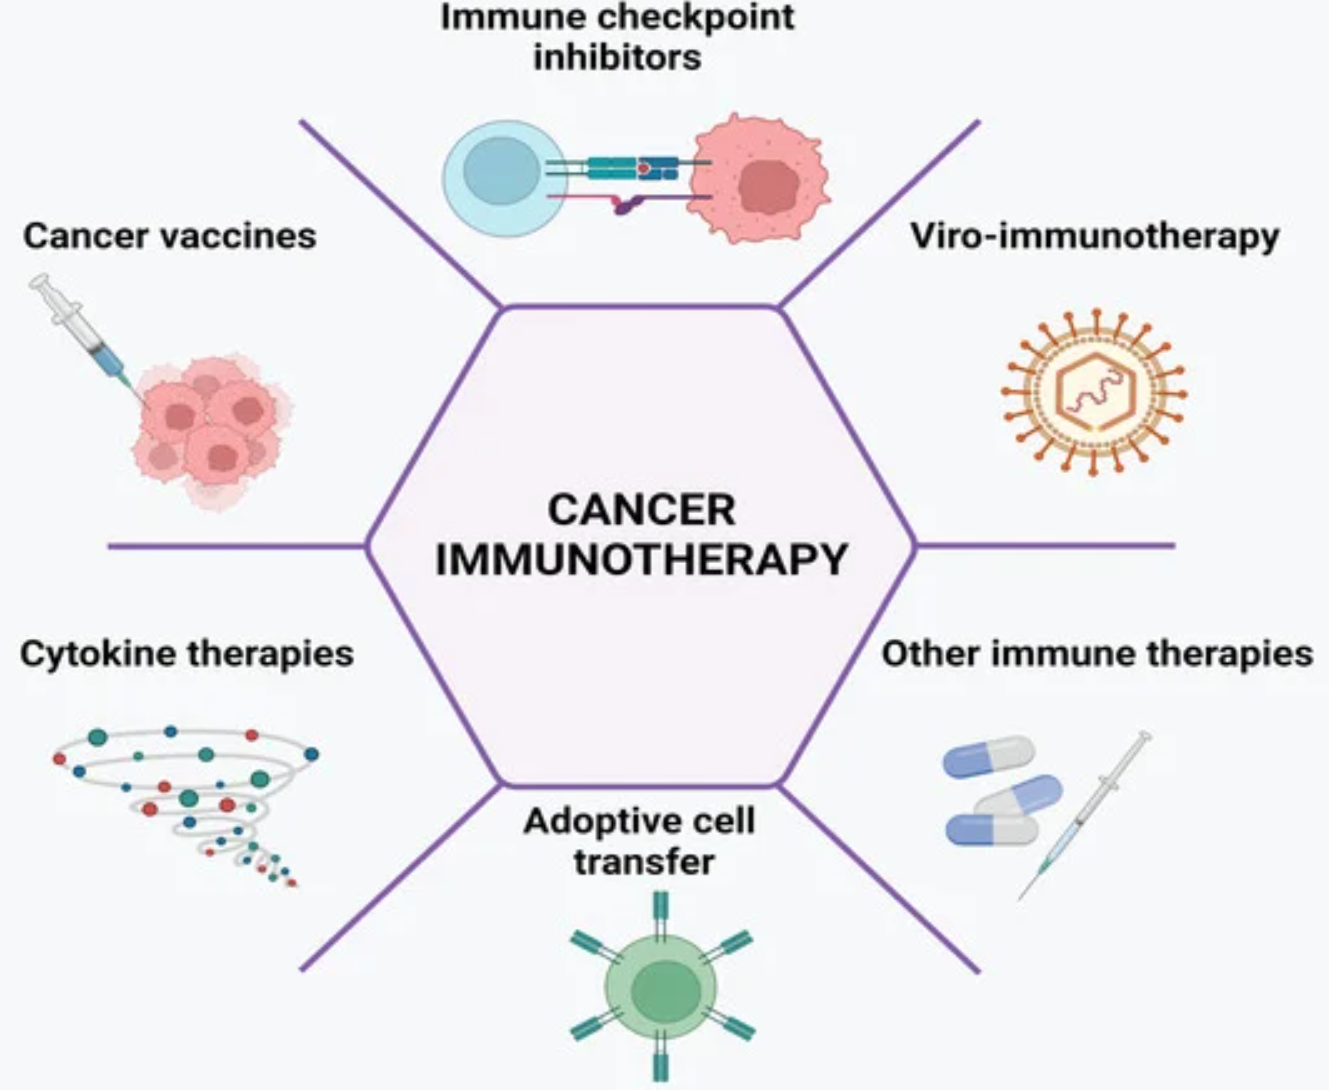
\includegraphics[width=0.7\textwidth]{../img/introduction/cancer_immunotherapy}
		\caption{Tipos de tratamientos para la inmunoterapia del cáncer. \textbf{Fuente}: \cite{kciuk2023recent}.}
	\end{figure}
\end{frame}
%-------------------------------------------------------
%-------------------------------------------------------


%%%%%%%%%%%%%%%%%%%%%%%%%%%%%%%%%%%%%%%%%%%%%%%%%%%%%%%%%%%%%%%%%%%%%%%%%%%%%%%%%%%%%%%%%%%%%%%%%%%%%%%%%%%%%%%%
\subsection{Vacunas Personalizadas}
%%%%%%%%%%%%%%%%%%%%%%%%%%%%%%%%%%%%%%%%%%%%%%%%%%%%%%%%%%%%%%%%%%%%%%%%%%%%%%%%%%%%%%%%%%%%%%%%%%%%%%%%%%%%%%%%




%-------------------------------------------------------
%-------------------------------------------------------
\begin{frame}{Contexto y Motivación}{Neoantígenos}
	Es una \textbf{proteína} que se forma en las células de Cáncer cuando ocurre mutaciones en el DNA  \cite{NCIdictionary2022, borden2022cancer}.
	
	\begin{figure}[]
		\centering
		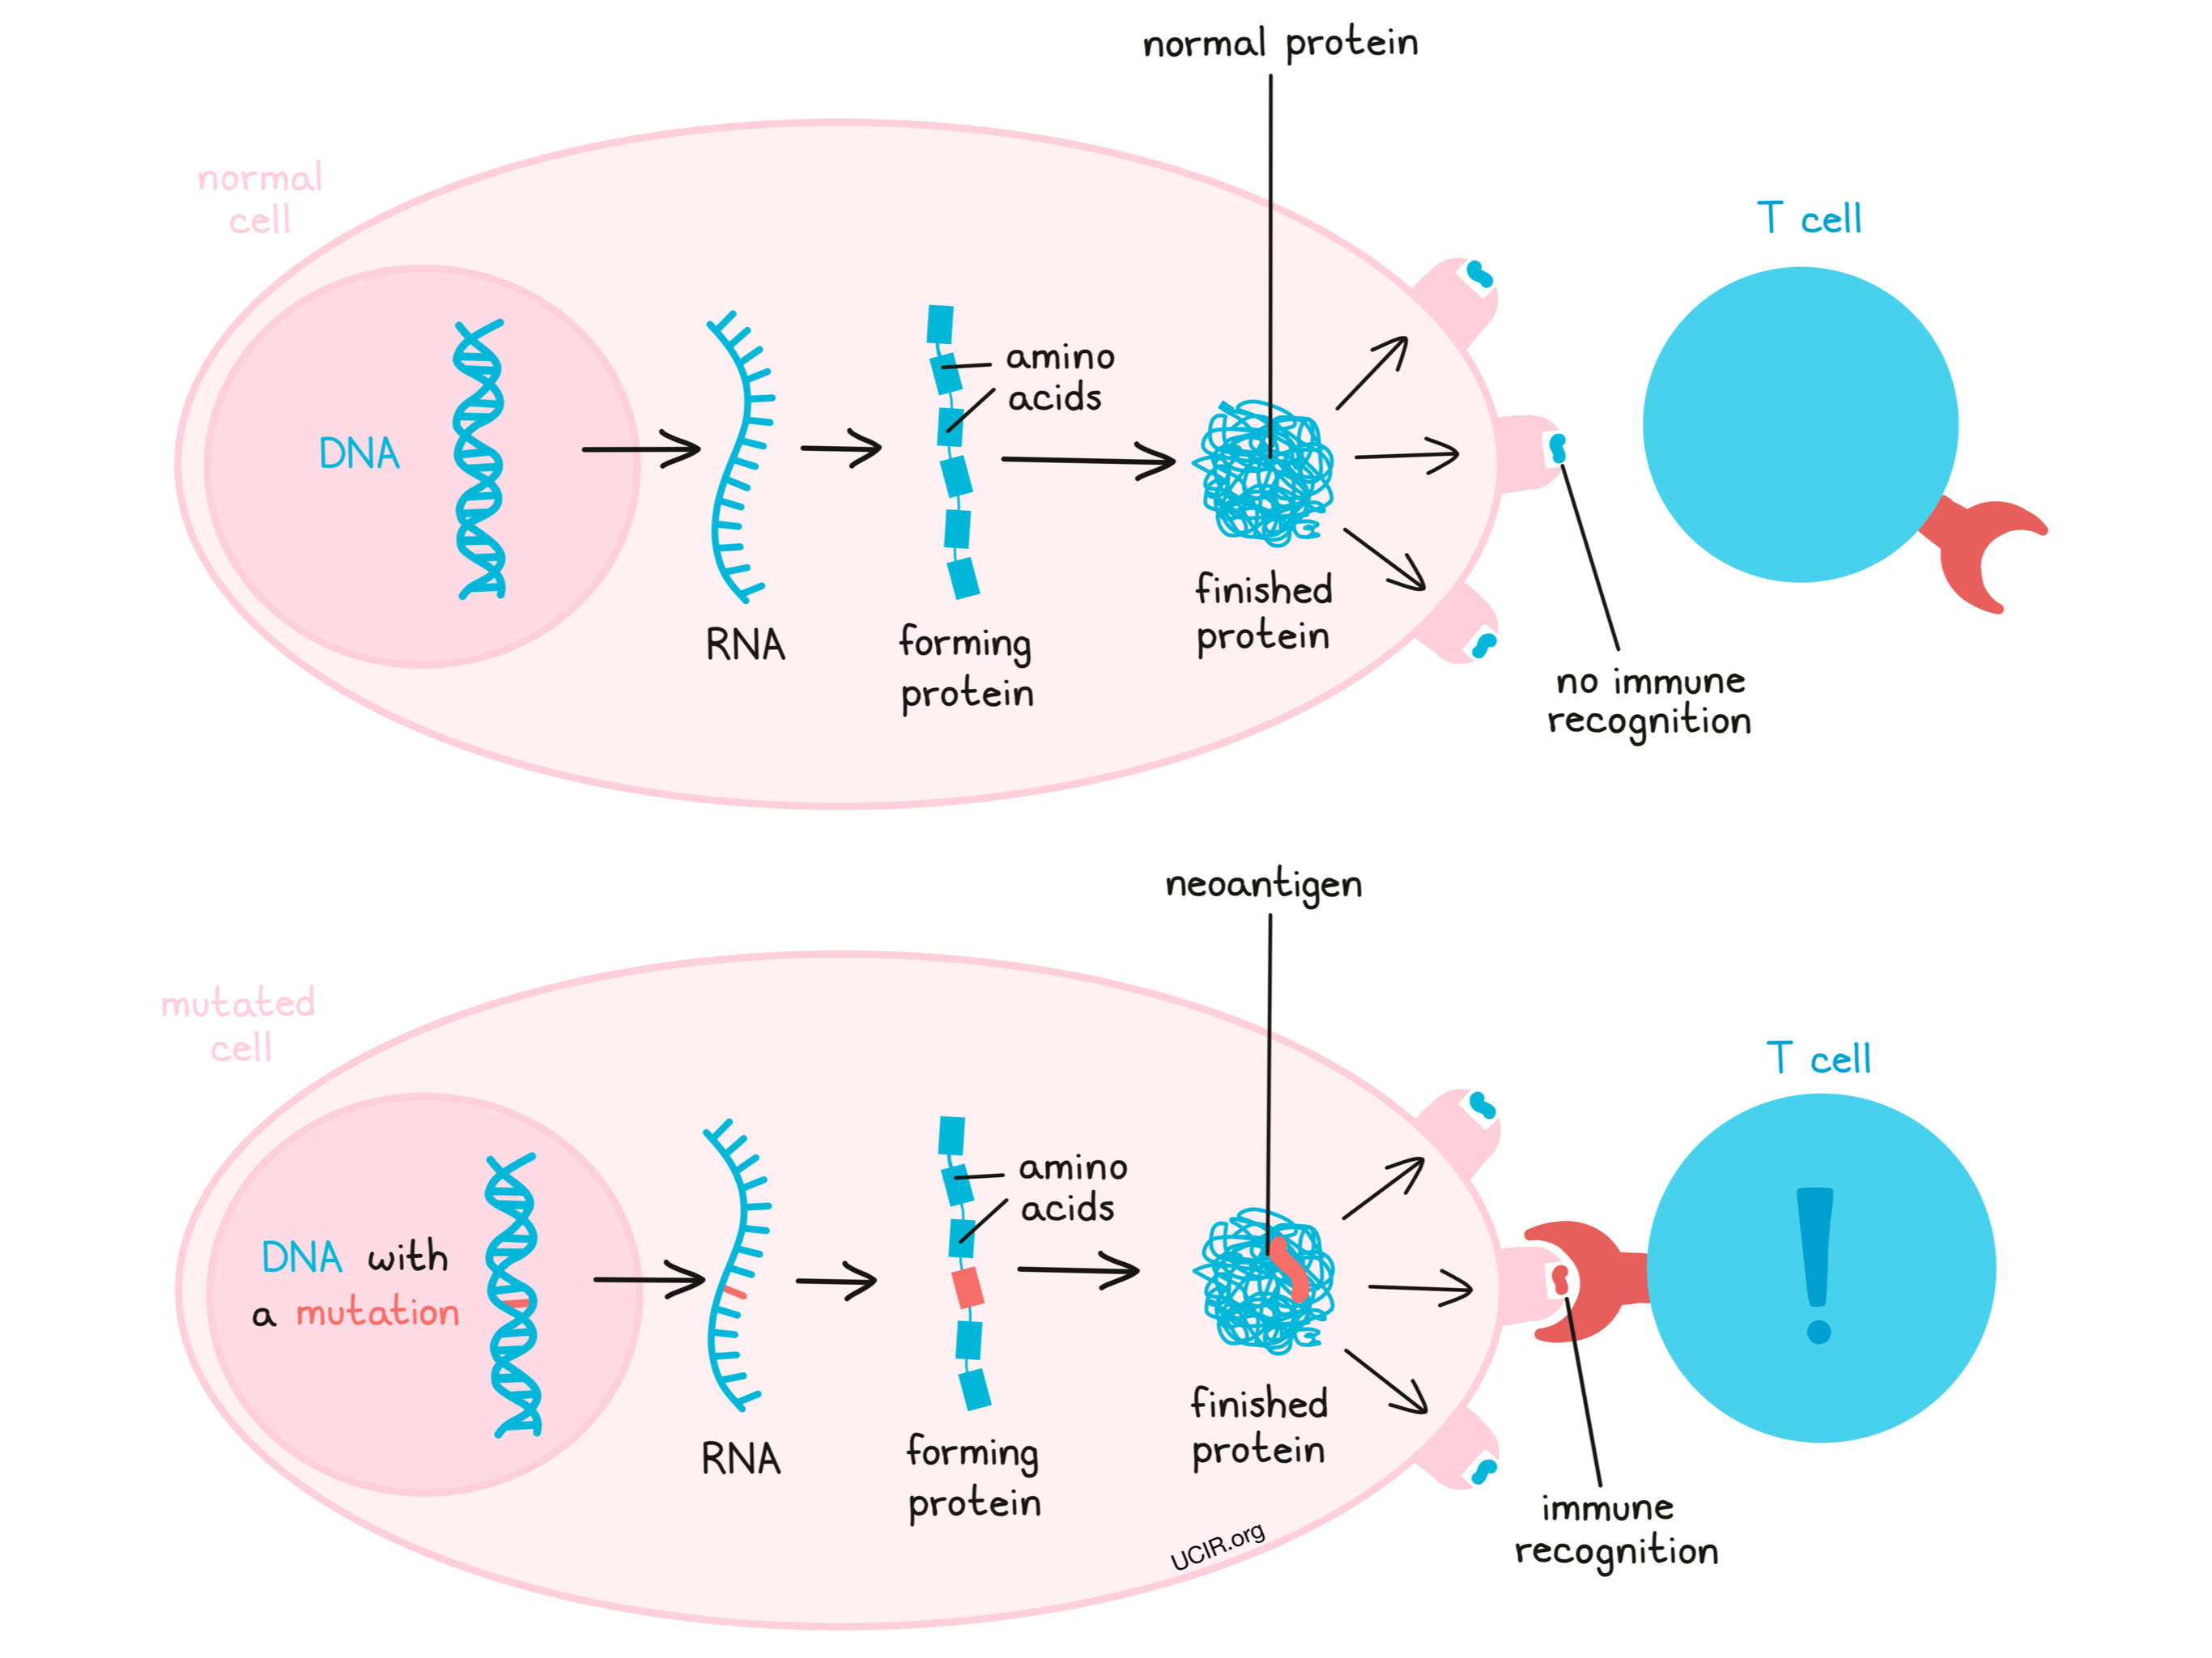
\includegraphics[width=0.7\textwidth]{../img/introduction/neoantigen}
		\caption{Neoantígenos y células T. \textbf{Fuente}: \cite{ucir2023}.}
	\end{figure}
\end{frame}
%-------------------------------------------------------
%-------------------------------------------------------

%-------------------------------------------------------
%-------------------------------------------------------
\begin{frame}{Contexto y Motivación}{Vacunas personalizadas}	
	\begin{figure}[H]
		\centering
		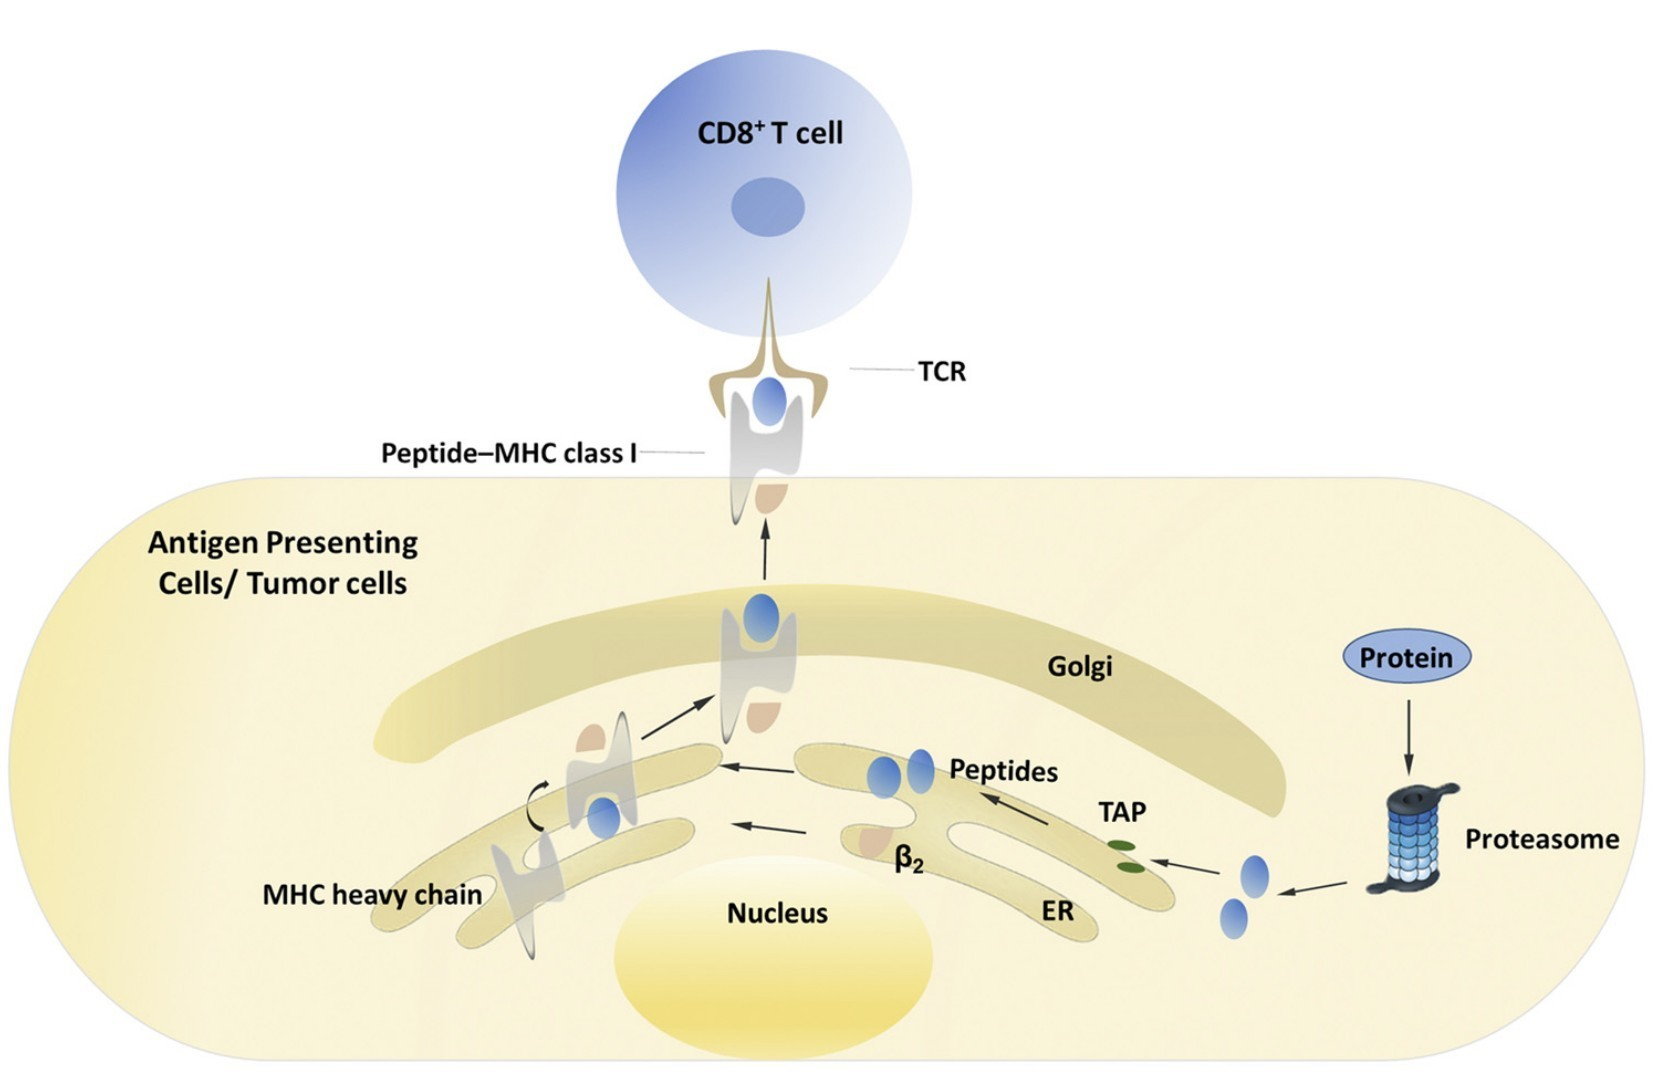
\includegraphics[width=0.9\textwidth]{../img/neoantigen/mhc1.jpg}
		\caption{Presentación de antígenos por MHC-I. Fuente: \cite{zhang2019application}}
		\label{fig:mhc1}
	\end{figure}	
\end{frame}
%-------------------------------------------------------
%-------------------------------------------------------

%%-------------------------------------------------------
%%-------------------------------------------------------
%\begin{frame}{MHC-II}{}		%
%	\begin{figure}[H]
	%		\centering
	%		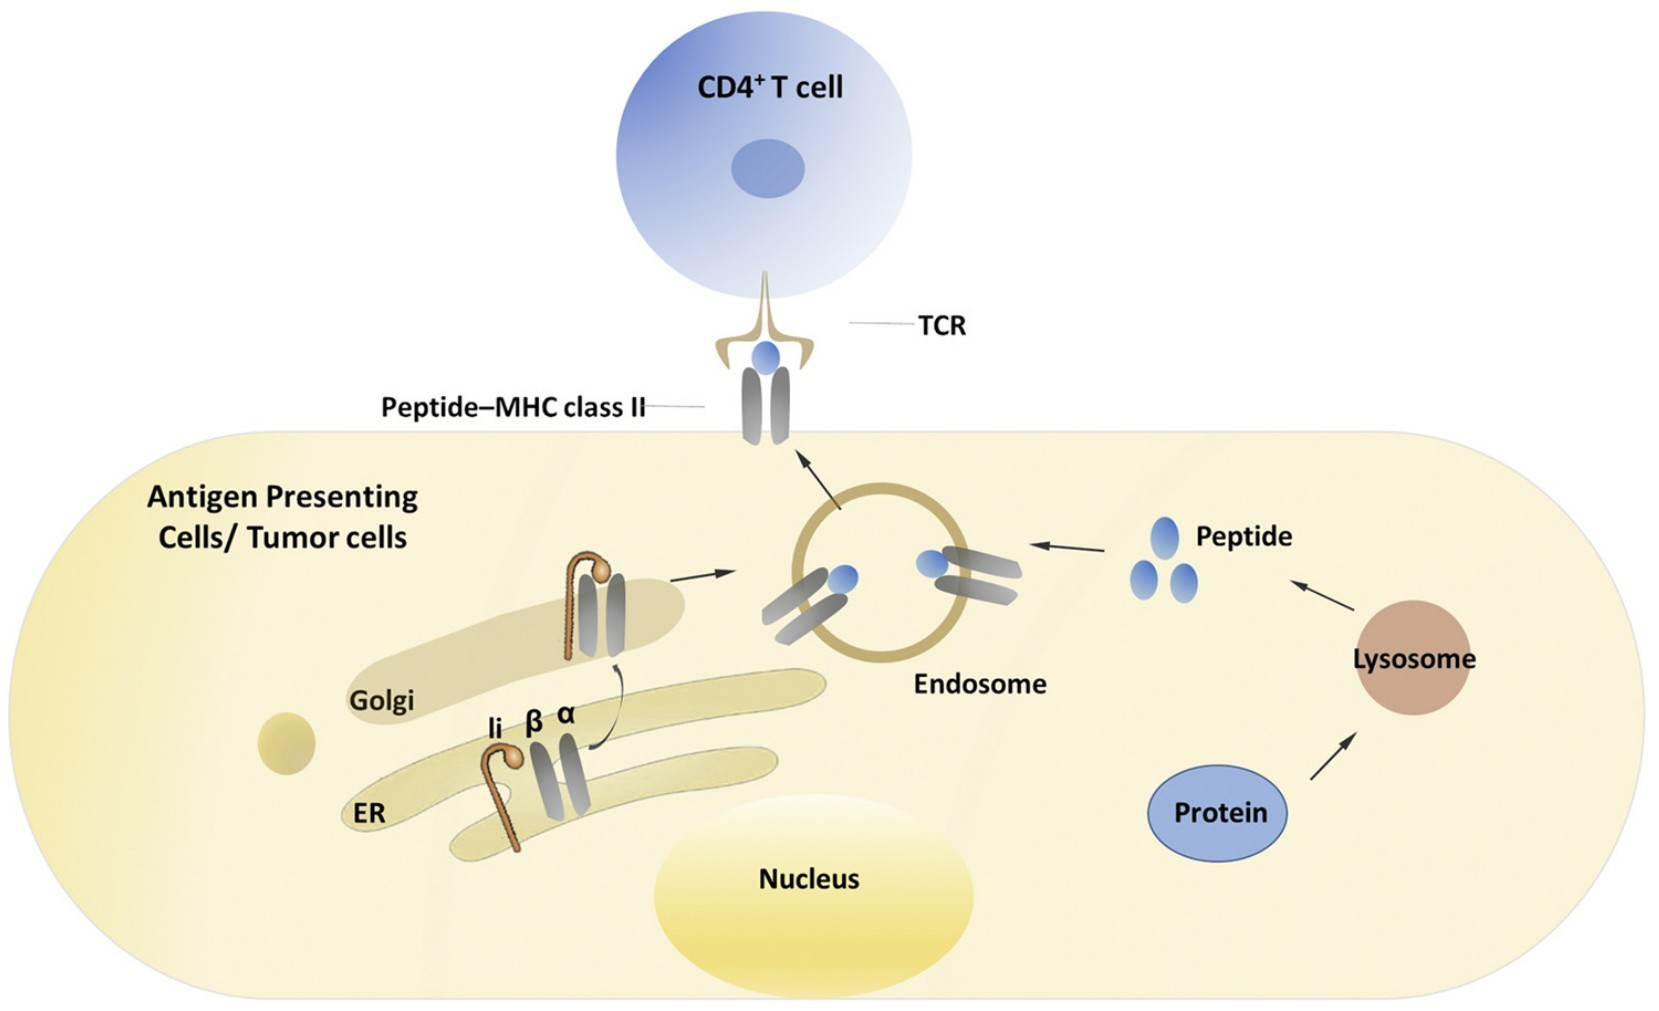
\includegraphics[width=0.9\textwidth]{../img/neoantigen/mhc2.jpg}
	%		\caption{Presentación de antígenos por MHC-II. Fuente: \cite{zhang2019application}}
	%		\label{fig:mhc2}
	%	\end{figure}	
%\end{frame}
%-------------------------------------------------------
%-------------------------------------------------------

%-------------------------------------------------------
%-------------------------------------------------------
\begin{frame}{Contexto y Motivación}{Vacunas personalizadas}	
	\begin{figure}[]
		\centering
		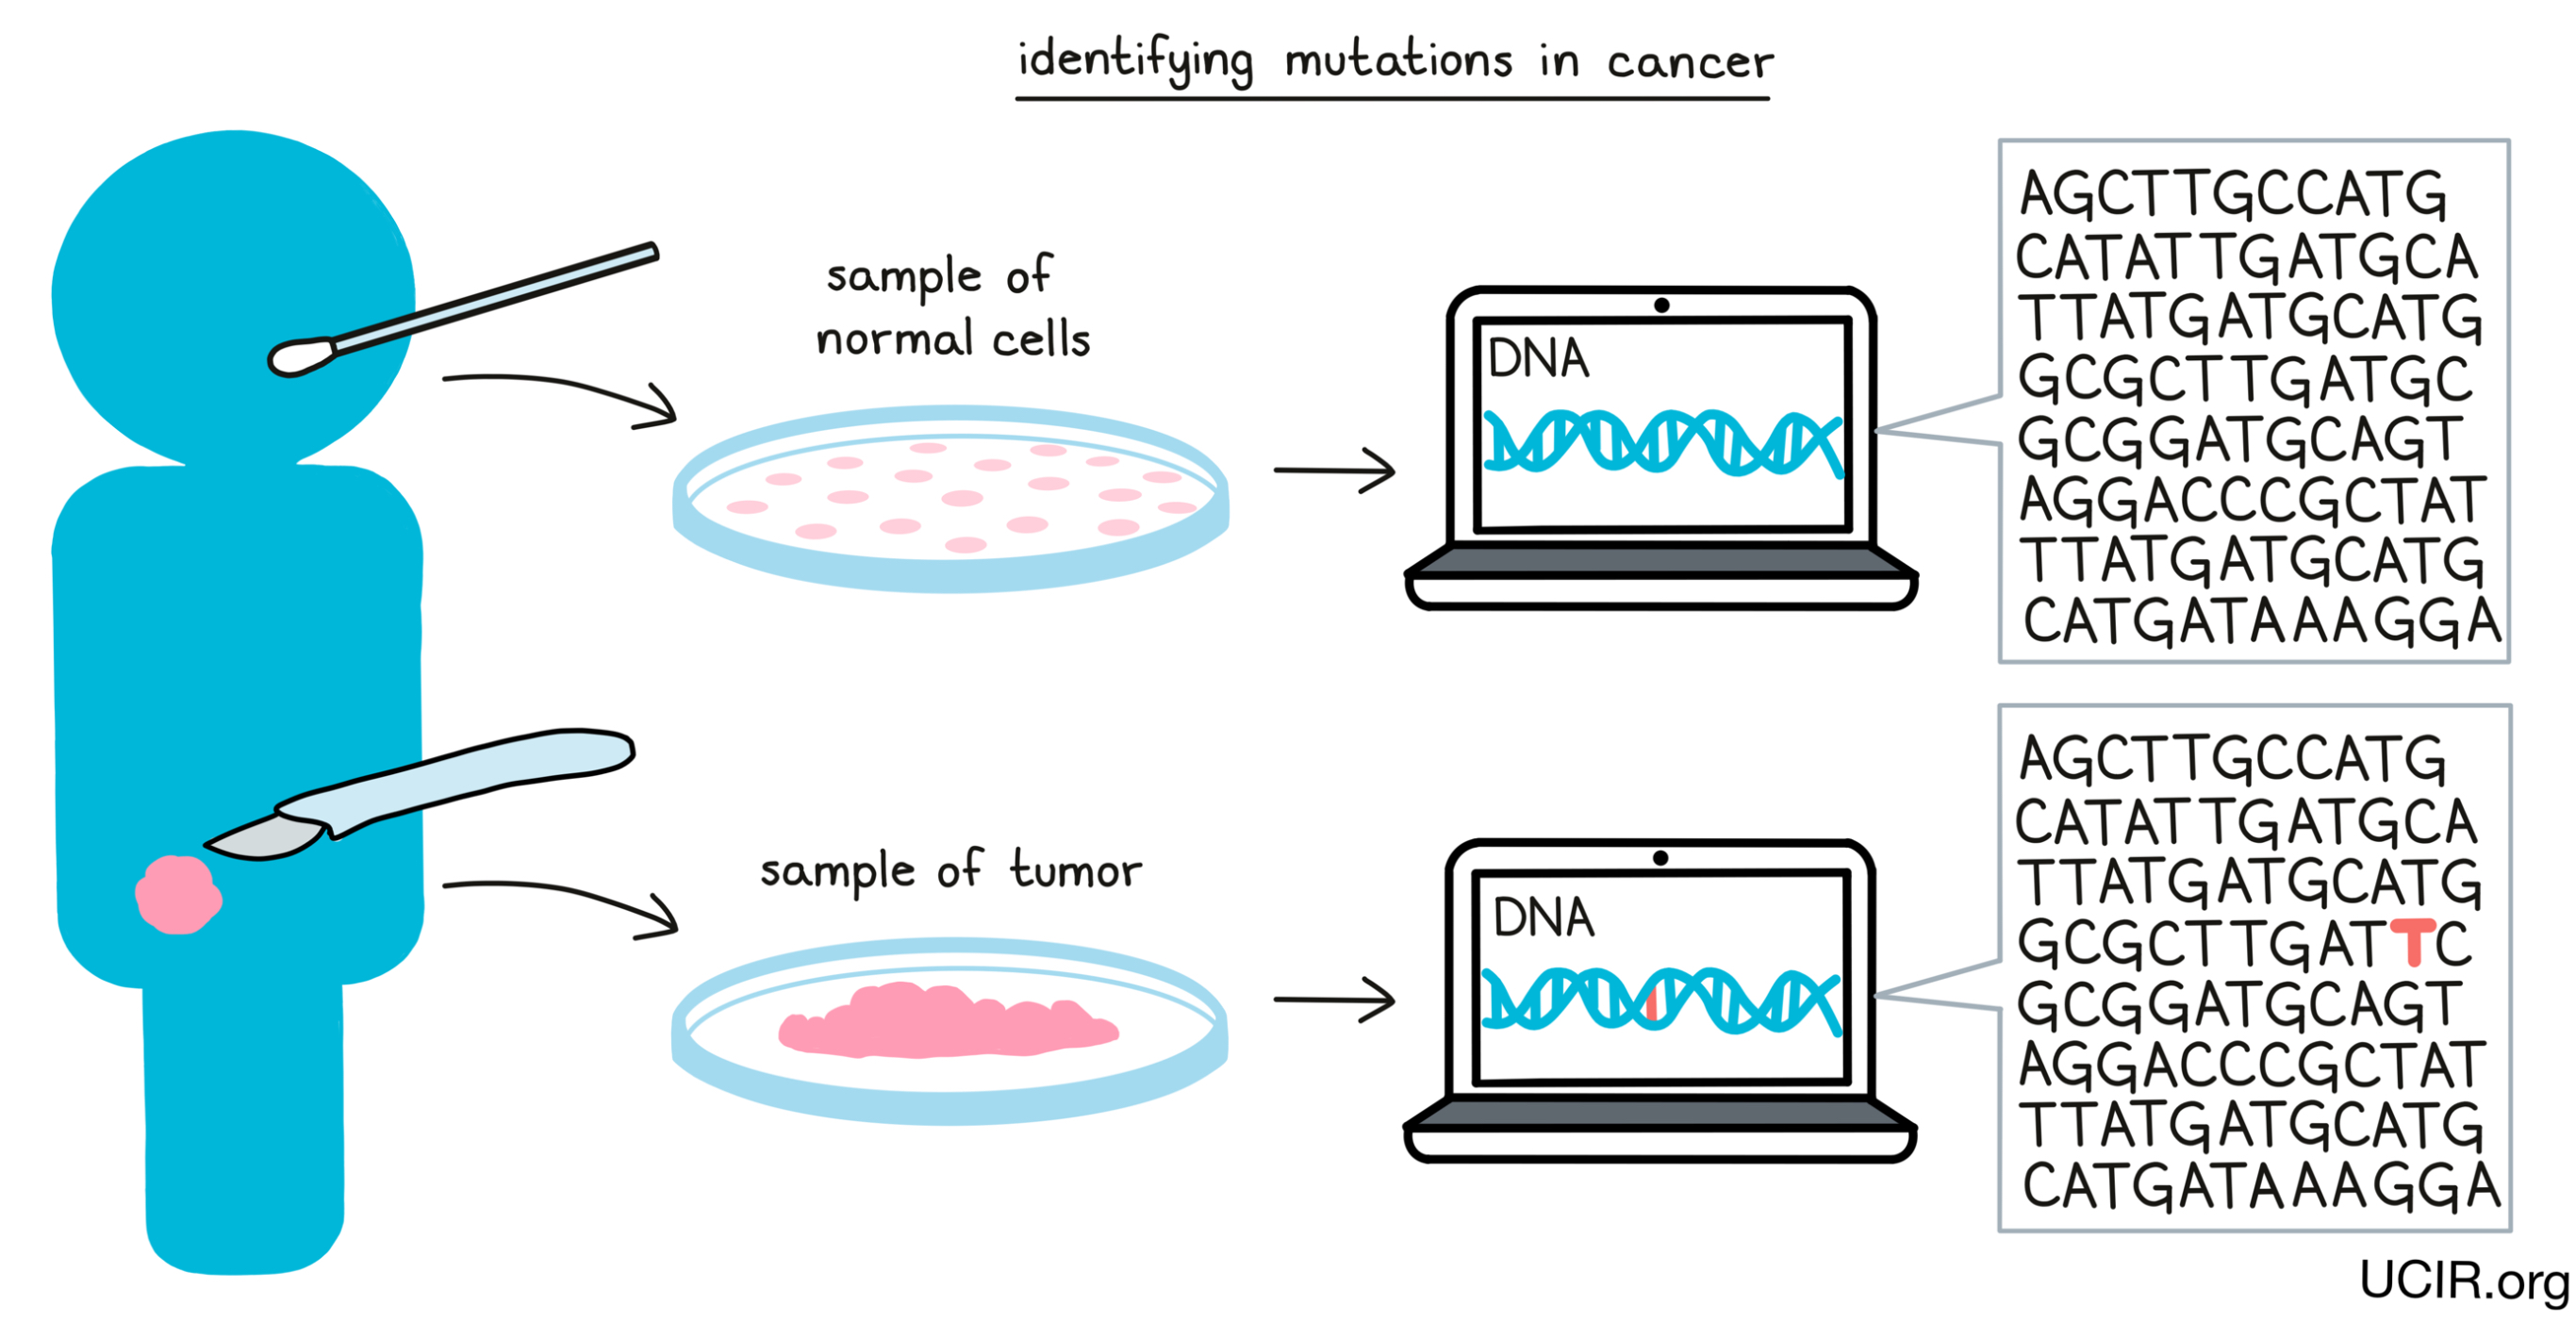
\includegraphics[width=\textwidth]{../img/introduction/vaccine_1}
		\caption{Proceso para la generación de vacunas contra el cáncer. \textbf{Fuente}: \cite{ucir2023}.}
	\end{figure}
\end{frame}
%-------------------------------------------------------
%-------------------------------------------------------



%-------------------------------------------------------
%-------------------------------------------------------
\begin{frame}{Contexto y Motivación}{Vacunas personalizadas}	
	\begin{figure}[]
		\centering
		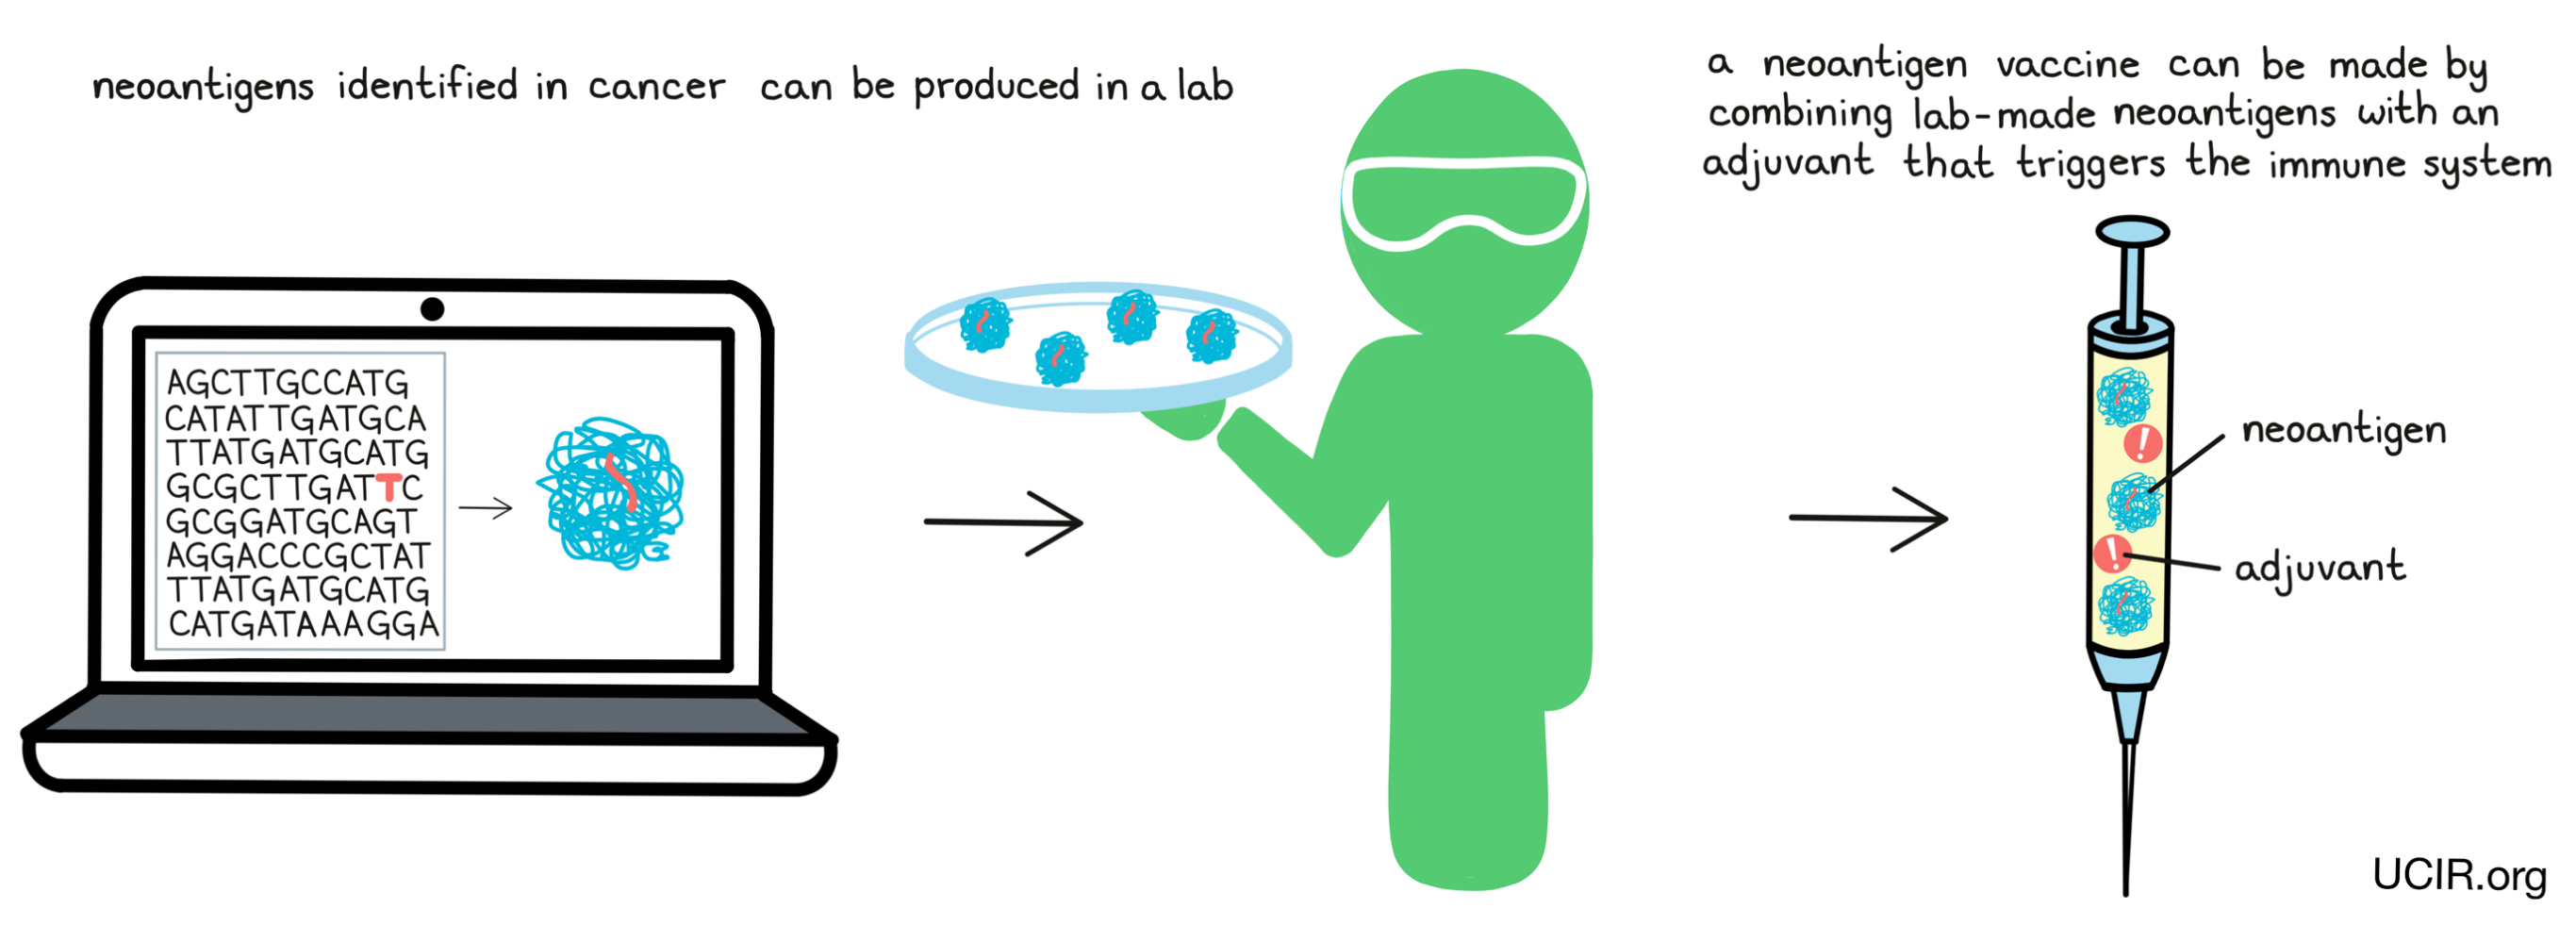
\includegraphics[width=\textwidth]{../img/introduction/vaccine_2}
		\caption{Proceso para la generación de vacunas contra el cáncer. \textbf{Fuente}: \cite{ucir2023}.}
	\end{figure}
\end{frame}
%-------------------------------------------------------
%-------------------------------------------------------

%-------------------------------------------------------
%-------------------------------------------------------
\begin{frame}{Contexto y Motivación}{Vacunas personalizadas}	
	\begin{figure}[]
		\centering
		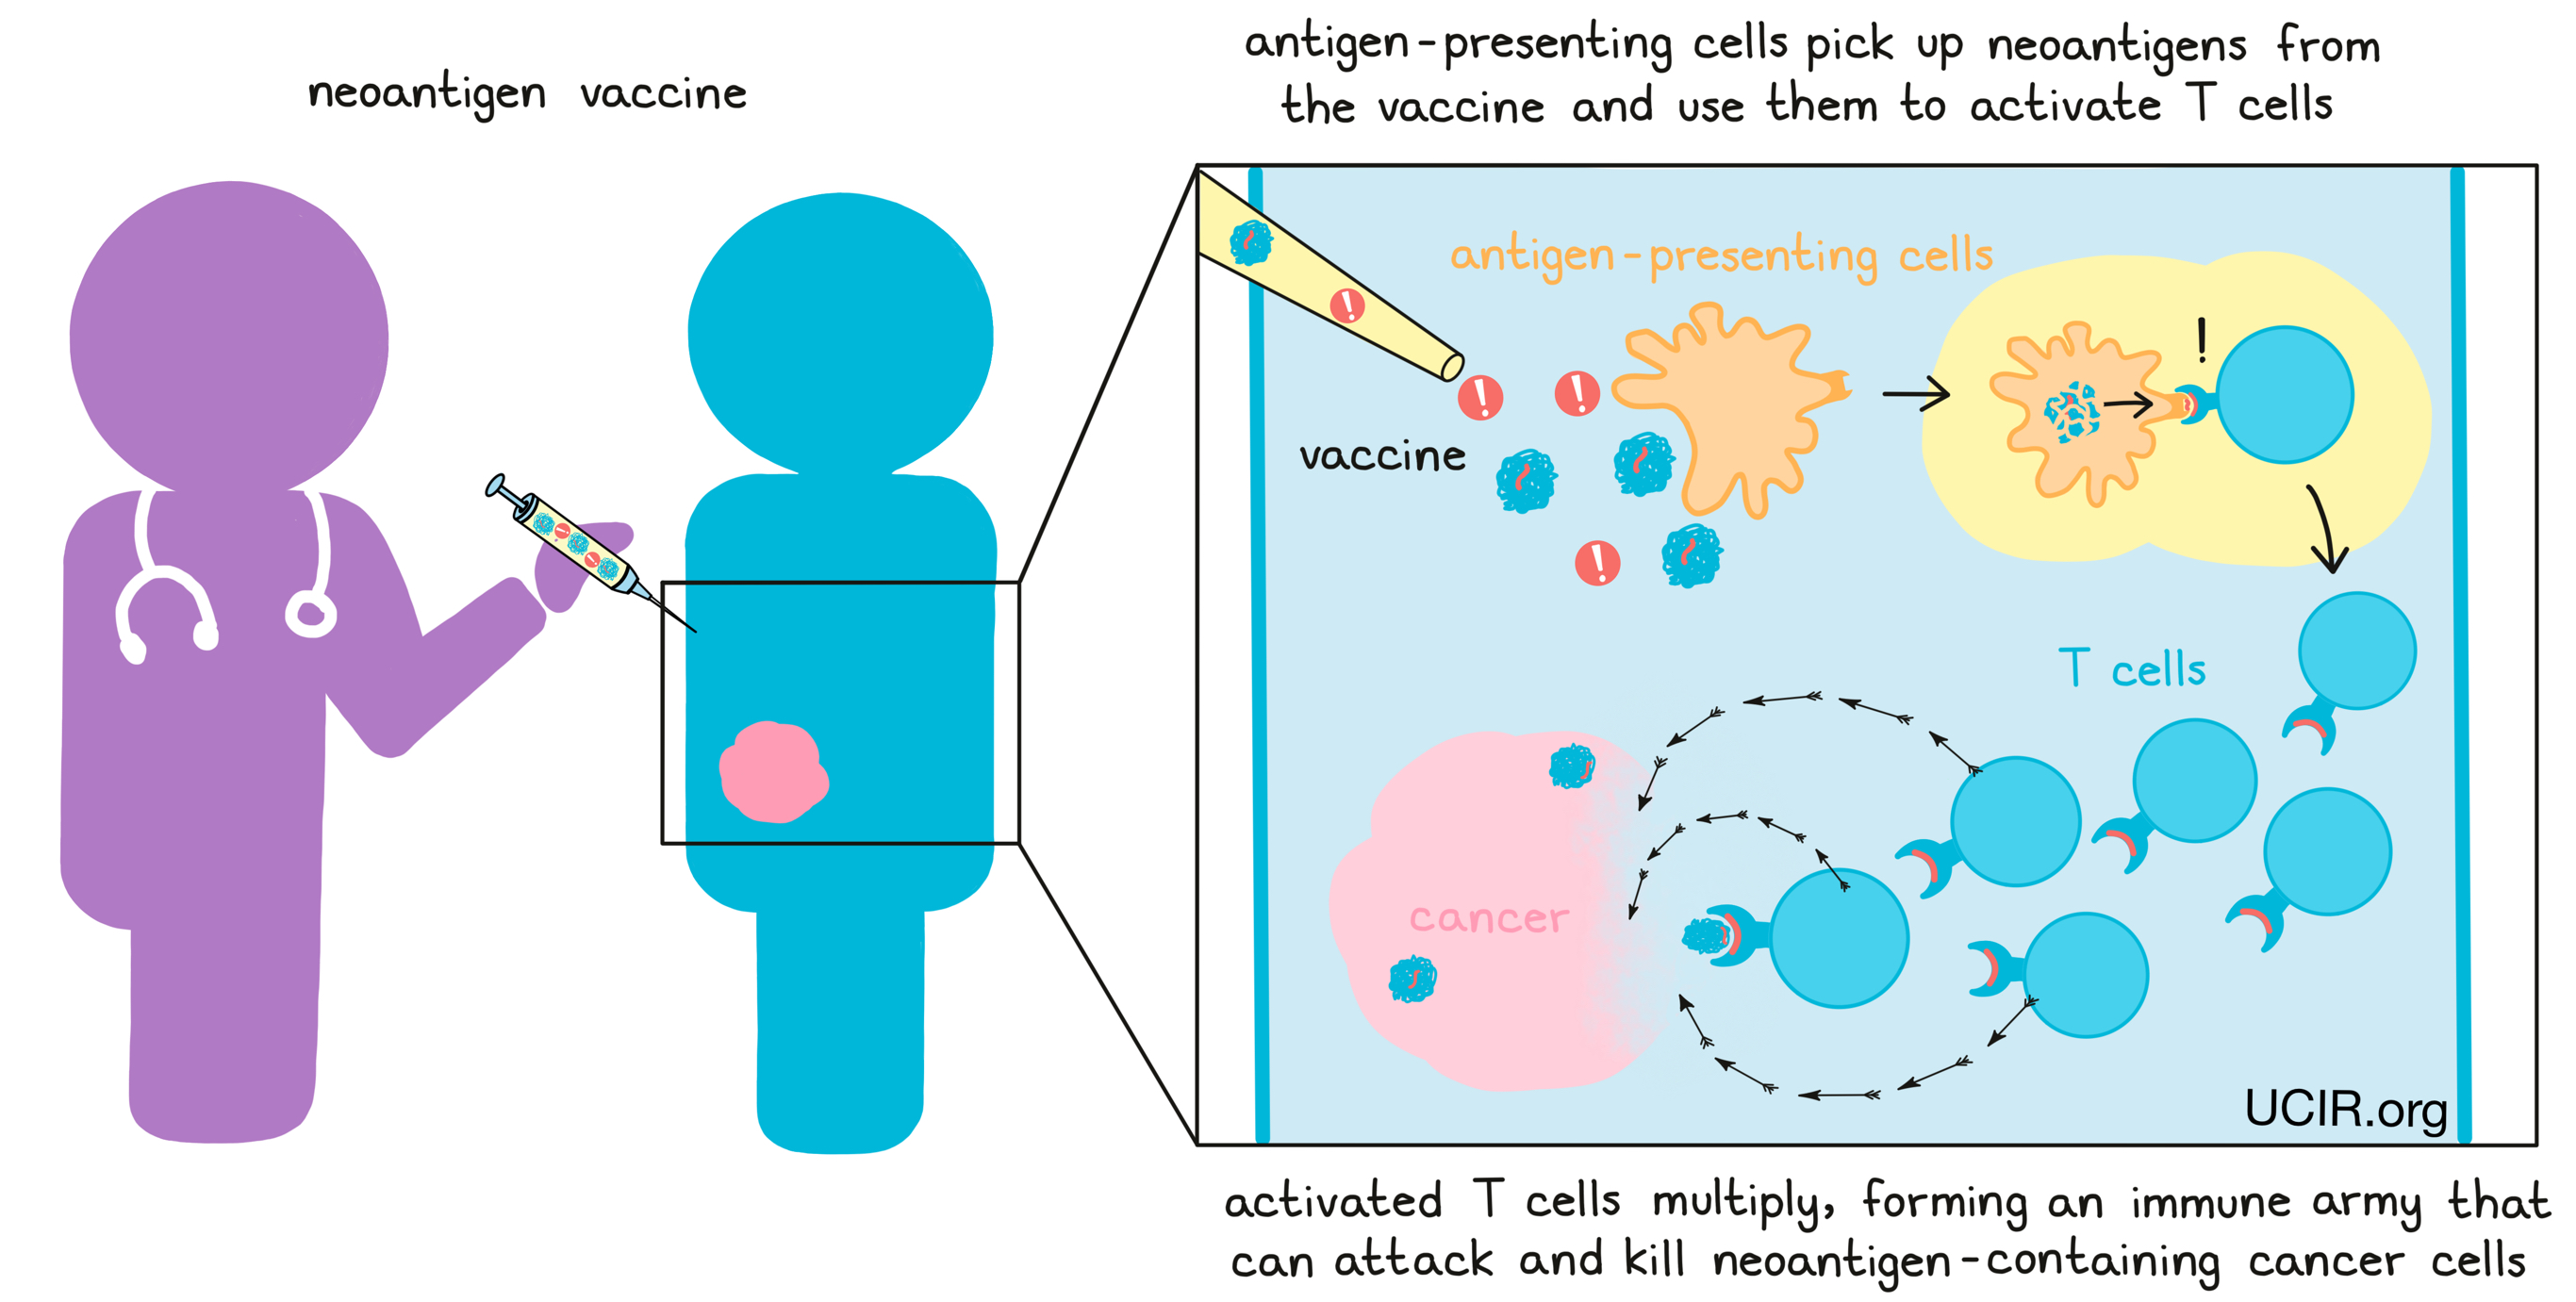
\includegraphics[width=\textwidth]{../img/introduction/vaccine_3}
		\caption{Proceso para la generación de vacunas contra el cáncer. \textbf{Fuente}: \cite{ucir2023}.}
	\end{figure}
\end{frame}
%-------------------------------------------------------
%-------------------------------------------------------

	%-------------------------------------------------------
%-------------------------------------------------------
\begin{frame}{Contexto y Motivación}{Vacunas personalizadas}
	\begin{figure}
		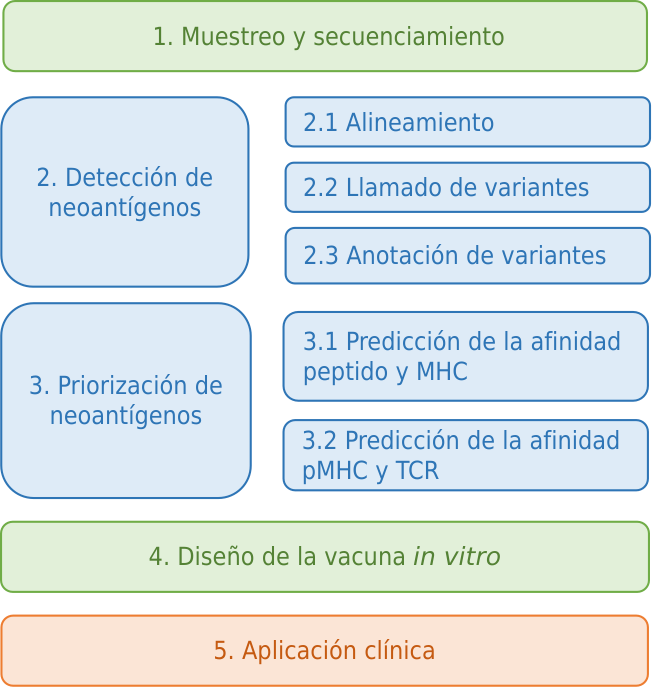
\includegraphics[width=0.5\textwidth]{../img/pipeline/pipeline_spanish}
		\caption{Resumen del proceso de  generación de vacunas contra el cáncer.}
	\end{figure}		
\end{frame}
%-------------------------------------------------------
%-------------------------------------------------------


	%%%%%%%%%%%%%%%%%%%%%%%%%%%%%%%%%%%%%%%%%%%%%%%%%%%%%%%%%%%%%%%%%%%%%%%%%%%%%%%%%%%%%%%%%%%%%%%%%%%%%%%%%%%%%%%%
%%%%%%%%%%%%%%%%%%%%%%%%%%%%%%%%%%%%%%%%%%%%%%%%%%%%%%%%%%%%%%%%%%%%%%%%%%%%%%%%%%%%%%%%%%%%%%%%%%%%%%%%%%%%%%%%
%%%%%%%%%%%%%%%%%%%%%%%%%%%%%%%%%%%%%%%%%%%%%%%%%%%%%%%%%%%%%%%%%%%%%%%%%%%%%%%%%%%%%%%%%%%%%%%%%%%%%%%%%%%%%%%%
\section{Problema y Objetivos}
%%%%%%%%%%%%%%%%%%%%%%%%%%%%%%%%%%%%%%%%%%%%%%%%%%%%%%%%%%%%%%%%%%%%%%%%%%%%%%%%%%%%%%%%%%%%%%%%%%%%%%%%%%%%%%%%
%%%%%%%%%%%%%%%%%%%%%%%%%%%%%%%%%%%%%%%%%%%%%%%%%%%%%%%%%%%%%%%%%%%%%%%%%%%%%%%%%%%%%%%%%%%%%%%%%%%%%%%%%%%%%%%%
%%%%%%%%%%%%%%%%%%%%%%%%%%%%%%%%%%%%%%%%%%%%%%%%%%%%%%%%%%%%%%%%%%%%%%%%%%%%%%%%%%%%%%%%%%%%%%%%%%%%%%%%%%%%%%%%
%-------------------------------------------------------
%-------------------------------------------------------
\begin{frame}{Problema}{}	
	\begin{block}{}
		\textbf{Menos del 5\%} de neoantígenos detectados activan el sistema inmune \cite{de2020neoantigen, mill2022neoms, bulik2019deep, bassani2015mass, yadav2014predicting}.
	\end{block}
	
	\pause
	\begin{block}{}
		\begin{itemize} 
			\item La no inclusión en conjunto de varias fuentes de información como DNA-seq, RNA-seq, y datos de MS \cite{kim2018neopepsee}. \pause
			\item  Uso herramientas de bajo desempeño para la predicción del enlace péptido-MHC (pMHC). La mayoría de aplicaciones, se basa en el uso de MHCFlurry \cite{o2020mhcflurry} y NetMHCpan4.1 \cite{reynisson2020netmhcpan}. \pause
			\item No consideran  la predicción del enlace pMHC-TCR  \cite{rubinsteyn2018computational}. \pause
			\item No utilizar información de eventos de \textit{alternative splicing}, variaciones estructurales y  fusión de genes \cite{wood2020neoepiscope}.
		\end{itemize}
	\end{block}
	
\end{frame}
%-------------------------------------------------------
%-------------------------------------------------------

%-------------------------------------------------------
%-------------------------------------------------------
\begin{frame}{Problema}{Formulación del problema}
	\begin{block}{}
		Es un problema de clasificación binaria que toma como entrada la secuencia de aminoácidos de un péptido ($p = \{A, ..., Q\}$) y el MHC ($q = \{A, N, ..., G\}$). Finalmente, necesitamos conocer la probabilidad de afinidad entre $p$ y $q$.
	\end{block}
	
	\begin{figure}
		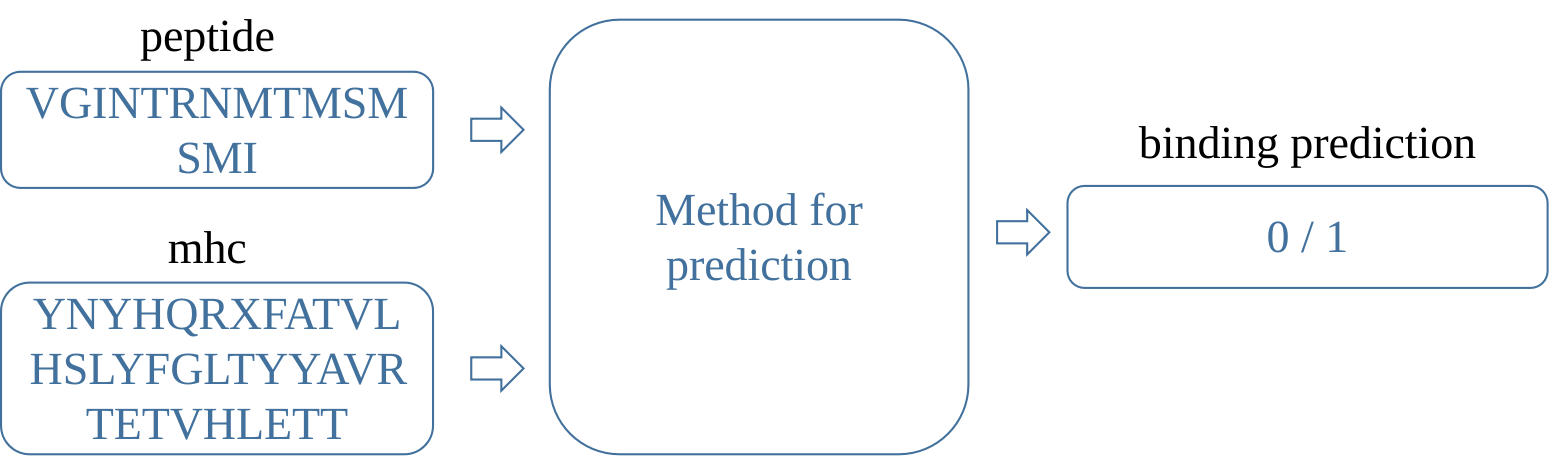
\includegraphics[width=0.9\textwidth]{../img/neoantigen/problem}
		\caption{Problema de predicción del enlace pMHC.}
	\end{figure}
\end{frame}
%-------------------------------------------------------
%-------------------------------------------------------


%-------------------------------------------------------
%-------------------------------------------------------
\begin{frame}{Objetivos}{}	
	\begin{block}{Objetivo general}
		Implementar un método \textit{in silico} basado en \textit{Transformers} y \textit{Transfer Learning} para la detección de neoantígenos, enfocados en la predicción de la unión pMHC. 
	\end{block}	

\end{frame}
%-------------------------------------------------------
%-------------------------------------------------------

%-------------------------------------------------------
%-------------------------------------------------------
\begin{frame}{Objetivos}{}	

	\begin{block}{Objetivos específicos}
		\begin{itemize} 
			\item Analizar los métodos que utilizan \textit{Transformers} para la predicción del enlace pMHC en el contexto de detección de neoantígenos. \pause
			\item Analizar los modelos basados en \textit{Transformers} TAPE, ProtBert-BFD, y EMS2 pre-entredados para diversas tareas en Proteómica y de los cuáles se puede aplicar \textit{Transfer Learning}. 	\pause
			\item Implementar \textit{fine-tuning} a los modelos TAPE, ProtBert-BFD, y EMS2 para la tarea de predicción del enlace pMHC, aplicando \textit{Gradient Accumulation Steps} (GAS) y una metodología de congelamiento de capas. \pause
			\item Comparar los modelos de mejor desempeño con las herramientas del estado del arte como: NetMHCpan4.1, MHCFlurry2.0, Anthem, ACME y MixMHCpred2.2.
		\end{itemize}
	\end{block}	
\end{frame}
%-------------------------------------------------------
%-------------------------------------------------------

%%%%%%%%%%%%%%%%%%%%%%%%%%%%%%%%%%%%%%%%%%%%%%%%%%%%%%%%%%%%%%%%%%%%%%%%%%%%%%%%%%%%%%%%%%%%%%%%%%%%%%%%%%%%%%%%
%%%%%%%%%%%%%%%%%%%%%%%%%%%%%%%%%%%%%%%%%%%%%%%%%%%%%%%%%%%%%%%%%%%%%%%%%%%%%%%%%%%%%%
\section{Estado del arte}
%%%%%%%%%%%%%%%%%%%%%%%%%%%%%%%%%%%%%%%%%%%%%%%%%%%%%%%%%%%%%%%%%%%%%%%%%%%%%%%%%%%%%%%%%%%%%%%%%%%%%%%%%%%%%%%%
%%%%%%%%%%%%%%%%%%%%%%%%%%%%%%%%%%%%%%%%%%%%%%%%%%%%%%%%%%%%%%%%%%%%%%%%%%%%%%%%%%%%%%

%-------------------------------------------------------
%-------------------------------------------------------
%\begin{frame}{Estado del arte}{Publicaciones sobre estudios de Neoantígenos}	
%		\begin{figure}
%		\centering
%		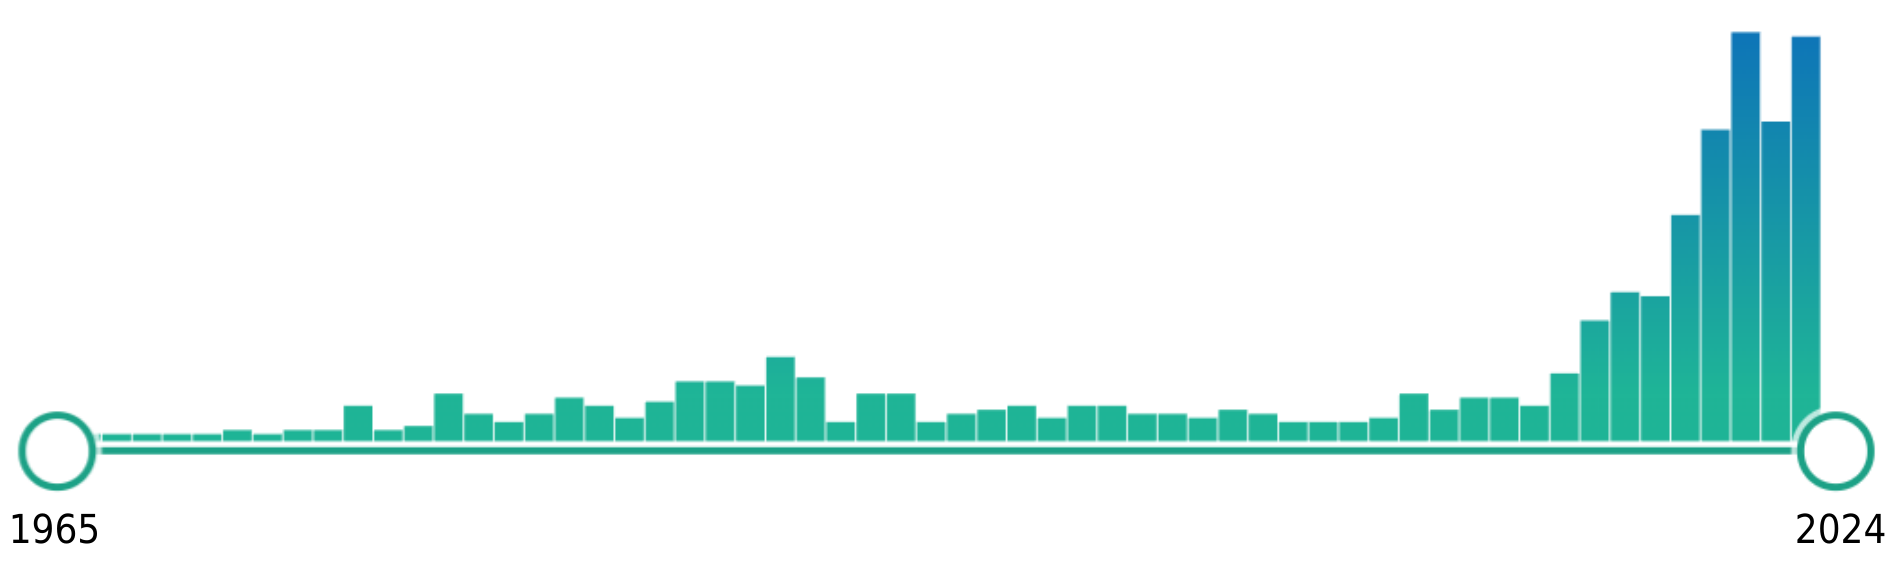
\includegraphics[width=\textwidth]{../img/state_of_art/papers_pubmed}	
%		\caption{Publicaciones sobre estudios de Neoantígenos. Fuente: PubMed.}
%	\end{figure}
%\end{frame}
%-------------------------------------------------------
%-------------------------------------------------------

%-------------------------------------------------------
%-------------------------------------------------------
%\begin{frame}{Estado del arte}{Publicaciones sobre estudios de predicción del enlace pMHC}	
%	\begin{figure}
%		\centering
%		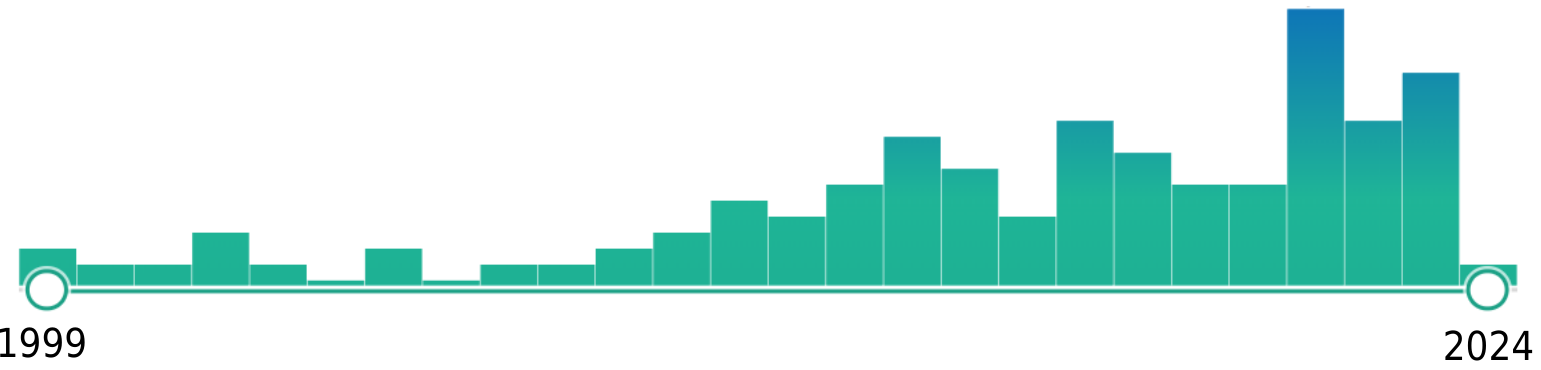
\includegraphics[width=\textwidth]{../img/state_of_art/papers_pubmed2}	
%		\caption{Publicaciones sobre estudios de predicción del enlace pMHC. Fuente: PubMed.}
%	\end{figure}
%\end{frame}
%-------------------------------------------------------
%-------------------------------------------------------


%-------------------------------------------------------
%-------------------------------------------------------
%\begin{frame}{Estado del arte}{Preguntas de investigación}
	
%	\begin{table}[h]
%		\begin{center}
%			\caption{Preguntas de investigación}
%			\label{tab:questions}
%			\setlength{\tabcolsep}{0.5em} % for the horizontal padding
%			{\renewcommand{\arraystretch}{1.4}% for the vertical padding
%				\begin{tabular}{p{8.5cm}}
%					\textbf{Preguntas de investigación} \\ \hline
%					\textbf{Q1}. ¿Como se aplican los modelos \textit{Transformers} para la detección de neoantígenos? \\
%					\textbf{Q2}. ¿Que problemas y limitaciones hacen frente los modelos \textit{Transformers} en la detección de neoantígenos? \\
%					\textbf{Q3}.  ¿Que \textit{pipelines} se han desarrollado para la detección de neoantígenos? \\
%					\textbf{Q4}.  ¿Que pruebas clínicas, de vacunas personalizadas de neoantígenos, han sido aplicadas? \\		
%				\end{tabular}
%			}
%		\end{center}
%	\end{table}
	
%\end{frame}
%-------------------------------------------------------
%-------------------------------------------------------

%-------------------------------------------------------
%-------------------------------------------------------
%\begin{frame}{Estado del arte}{Cadena de busqueda}
	
%	\begin{table}[]
%		\caption{Cadenas de búsqueda utilizadas para cada fase de detección de neoantígenos.}
%		\label{tab:search}
%		\centering
%		\tiny
%		\setlength{\tabcolsep}{0.5em} % para el espaciado horizontal
%		{\renewcommand{\arraystretch}{1.7}% para el espaciado vertical
%			\begin{tabular}{p{3cm}p{7cm}}
%				\textbf{Categoría} & \textbf{Cadena de búsqueda} \\ \hline
%				Priorización de neoantígenos & \textit{(mhc OR hla) AND (peptide OR epitope OR antigen) AND (specificity OR immunogenicity OR binding OR affinity OR predict* OR detection OR presentation OR classification) AND (transformer* OR bert* OR attention OR 'transfer learning' OR method* OR predict*)'', ( tcr OR 't cell' OR t-cell) AND (mhc OR peptide OR epitope OR antigen) AND (specificity OR immunogenicity OR binding OR affinity OR predict* OR detection OR presentation OR classification) AND (transformer* OR bert* OR attention OR 'transfer learning' OR method* OR predict*)} \\
				
				
%				\textit{Pipelines} & \textit{(pipeline OR toolkit) AND ( tcr OR 't cell' OR t-cell OR mhc OR hla OR peptide OR epitope OR antigen* OR neoantigen*) (pipeline OR tool* OR workflow OR application OR web* ) AND ( peptide OR epitope OR antigen* OR neoantigen* OR neoepito*) AND (immunotherapy OR detection OR identify* OR predict* OR presentation*)}\\
				
%				Ensayos clínicos &  \textit{(neoantigen OR neoepitope OR denditric cell) AND (vaccines OR immunology)}
				
%		\end{tabular}}
%	\end{table}
%\end{frame}
%-------------------------------------------------------
%-------------------------------------------------------


%-------------------------------------------------------
%-------------------------------------------------------
%\begin{frame}{Estado del arte}{Bases de datos de búsqueda}
	
%	\begin{table}[H]
%		\centering
%		\begin{center}
%			\caption{Bases de datos utilizadas en la RSL.}
%			\label{tab:bd_RSL}
%			\setlength{\tabcolsep}{0.5em} % for the horizontal padding
%			{\renewcommand{\arraystretch}{1.2}% for the vertical padding
%				\begin{tabular}{p{3cm}}
%					\textbf{Bases de datos} \\ \hline
%					PubMed                                                                               \\
%					Scopus \\				
%					Google schoolar          \\
%					Web of Science                                                                                               
%				\end{tabular}
%			}
%		\end{center}
%	\end{table}
	
%\end{frame}
%-------------------------------------------------------
%-------------------------------------------------------



%-------------------------------------------------------
%-------------------------------------------------------
%\begin{frame}{Estado del arte}{Criterios de inclusión}
	
%\begin{table}[h]
%	\begin{center}
%		\caption{Criterios de inclusión y exclusión.}
%		\label{tab:criterios}
%		\scriptsize
%		\setlength{\tabcolsep}{0.5em} % for the horizontal padding
%		{\renewcommand{\arraystretch}{1.5}% for the vertical padding
%			\begin{tabular}{p{5cm}p{5cm}}
%				\textbf{Criterio de inclusión}                                                   & \textbf{Criterio de exclusión}                                                           \\ \hline
%				Artículos en revistas Q1 o Q2 según Scimago o Conferencias ERA (A o B). & Artículos de Conferencias de bajo nivel.  \\
				
%				Artículos publicados desde el 2018. & Publicaciones que no son del área de computación o Bioinformática. \\      
				
%				Artículos que hagan uso de \textit{Transformers} o \textit{Deep Learning} con mecanismos de atención. & \\                                                                                                 
%			\end{tabular}
%		}
%	\end{center}
%\end{table}
	
\end{frame}
%-------------------------------------------------------
%-------------------------------------------------------


%-------------------------------------------------------
%-------------------------------------------------------
\begin{frame}{Estado del arte}{\textit{Papers} seleccionados}
        \begin{block}{}
            Se establecieron, preguntas de investigación, criterios de inclusión, cadenas de búsqueda y se busco en PudMed, Scopus y Google Schoolar.
        \end{block}

	\begin{block}{}
		Primer filtro por título (\textbf{151 artículos}). Luego, según los criterios de inclusión y lectura del \textit{abstract} se obtuvo \textbf{79 artículos}.
	\end{block}

	
\end{frame}
%-------------------------------------------------------
%-------------------------------------------------------



%-------------------------------------------------------
%-------------------------------------------------------
\begin{frame}{Estado del arte}{Resumen}
	
	%\fontsize{12pt}{10pt}\selectfont
	
	\begin{table}[]
		\caption{Redes \textit{Transformers} utilizadas en la predicción del enlace pMHC.}
		\label{tab:transformes}
		\setlength{\tabcolsep}{0.6em} % for the horizontal padding
		{\renewcommand{\arraystretch}{1.6}% for the vertical padding
			
			\begin{footnotesize}
				\begin{tabular}{p{1cm}p{1.5cm}p{7cm}}
					\multicolumn{1}{l}{\textbf{Año}}                                   & \textbf{Nombre}                       & \textbf{Modelo}     \\  \hline
					
					2022\cite{zhang2022hlab}&	\textbf{HLAB}&	BERT de ProtBert en cascada con BiLSTM.	\\
					
					2022\cite{wang2022mhcroberta}          & MHC RoBERTa             &  RoBERTa  pre-entrenado y seguido de 12 \textit{multi-head} SA y una capa lineal.                                                                                     \\
					2022\cite{chu2022transformer}          & TransPHLA                     & Usa SA basado en cuatro bloques. \\
					
					2021\cite{gasser2021interpreting}  & \textbf{ImmunoBERT}                              & BERT TAPE pre-entrenado y seguido de una capa lineal. Se enfocó en pMHC-I.  \\
					
					2021\cite{cheng2021bertmhc}             & \textbf{BERTMHC}                            & BERT TAPE pre-entrenado y seguido de una capa lineal. Se enfocó en pMHC-II. \\
					
				\end{tabular}
			\end{footnotesize}
		}
	\end{table}
	
	
\end{frame}
%-------------------------------------------------------
%-------------------------------------------------------



%%%%%%%%%%%%%%%%%%%%%%%%%%%%%%%%%%%%%%%%%%%%%%%%%%%%%%%%%%%%%%%%%%%%%%%%%%%%%%%%%%%%%%%%%%%%%%%%%%%%%%%%%%%%%%%%
%%%%%%%%%%%%%%%%%%%%%%%%%%%%%%%%%%%%%%%%%%%%%%%%%%%%%%%%%%%%%%%%%%%%%%%%%%%%%%%%%%%%%%
\section{Propuesta}
%%%%%%%%%%%%%%%%%%%%%%%%%%%%%%%%%%%%%%%%%%%%%%%%%%%%%%%%%%%%%%%%%%%%%%%%%%%%%%%%%%%%%%%%%%%%%%%%%%%%%%%%%%%%%%%%
%%%%%%%%%%%%%%%%%%%%%%%%%%%%%%%%%%%%%%%%%%%%%%%%%%%%%%%%%%%%%%%%%%%%%%%%%%%%%%%%%%%%%%

%-------------------------------------------------------
%-------------------------------------------------------
\begin{frame}{Propuesta}{}

	\begin{figure}[H]
		\centering
		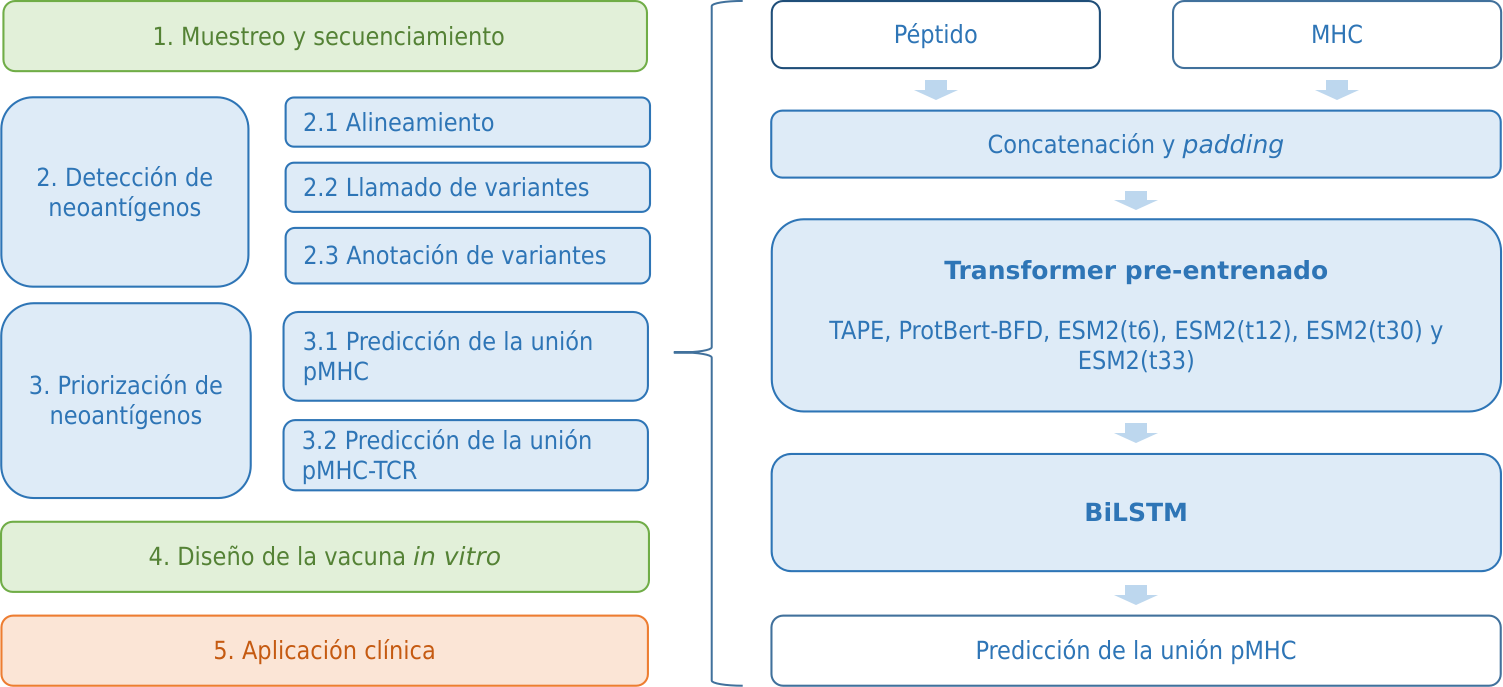
\includegraphics[width=\textwidth]{../img/proposal/proposal}	
		\caption{Propuesta para la predicción del enlace pMHC.}
		\label{fig:neo_det_seq}
	\end{figure}
\end{frame}
%-------------------------------------------------------
%-------------------------------------------------------


%-------------------------------------------------------
%-------------------------------------------------------
\begin{frame}{Propuesta}{\textit{Fine-tuning}}
	
	\begin{figure}
		\centering
		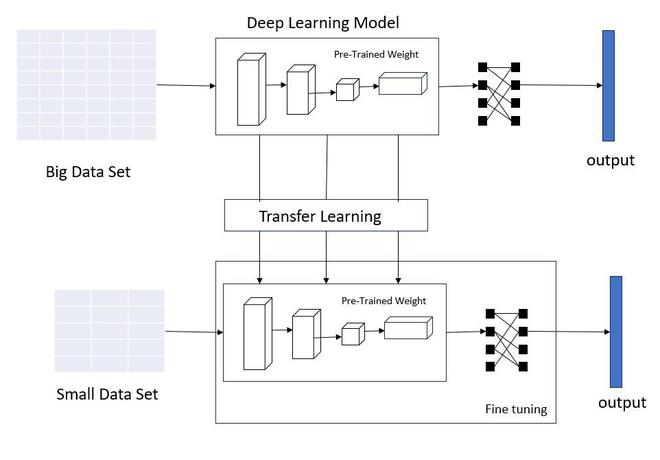
\includegraphics[width=0.8\textwidth]{../img/proposal/fine-tuning}	
		\caption{Ejemplo de \textit{Fine-tuning}. Fuente: \cite{prince2023understanding}.}		
	\end{figure}
	
\end{frame}
%-------------------------------------------------------
%-------------------------------------------------------

%-------------------------------------------------------
%-------------------------------------------------------
\begin{frame}{Propuesta}{\textit{Fine-tuning}}
	
	\begin{block}{}
		La arquitectura BERT, precede a un bloque BiLSTM. Este está compuesto por\textbf{ dos capas con 768 unidades} (inspirados en HLAB \cite{zhang2022hlab}).
	\end{block}

	\begin{block}{}
		Se utilizo los siguientes hiperparametros:
		\begin{itemize}
			\item $lr = 5e^{-5}$.
			\item \textit{weight decay} $ =0.0001$ (regularización).
			%\item \textit{momentum} $= 0.9$.
			\item \textit{linear warn-up steps} de 1000.
			\item Optimizador ADAM: ($\beta_1 = 0.9, \beta_2=0.999$).
			\item \textit{Early stopping}.
		\end{itemize}
	
		  Estos valores fueron utilizados por BERTMHC \cite{cheng2021bertmhc} después de buscar los mejores parámetros utilizando \textit{grid search}.
	\end{block}
	
\end{frame}
%-------------------------------------------------------
%-------------------------------------------------------

%-------------------------------------------------------
%-------------------------------------------------------
\begin{frame}{Propuesta}{Ambiente de trabajo}
	
	\begin{block}{Librerías}
		Se utilizó \textbf{PyTorch 1.13} y\textbf{ Python 3.9} para definir los modelos de \textit{deep learning}.
	\end{block}
	
	\begin{block}{GPU}
		Se utilizo dos GPU: 
		\begin{itemize}
			\item GPU propia: RTX3070 (8GB).
			\item GPU de la plataforma Paperspace.
		\end{itemize}
	\end{block}
\end{frame}
%-------------------------------------------------------
%-------------------------------------------------------

%-------------------------------------------------------
%-------------------------------------------------------
\begin{frame}{Propuesta}{\textit{Gradient Accumulation Steps}}
		\begin{figure}
		\centering
		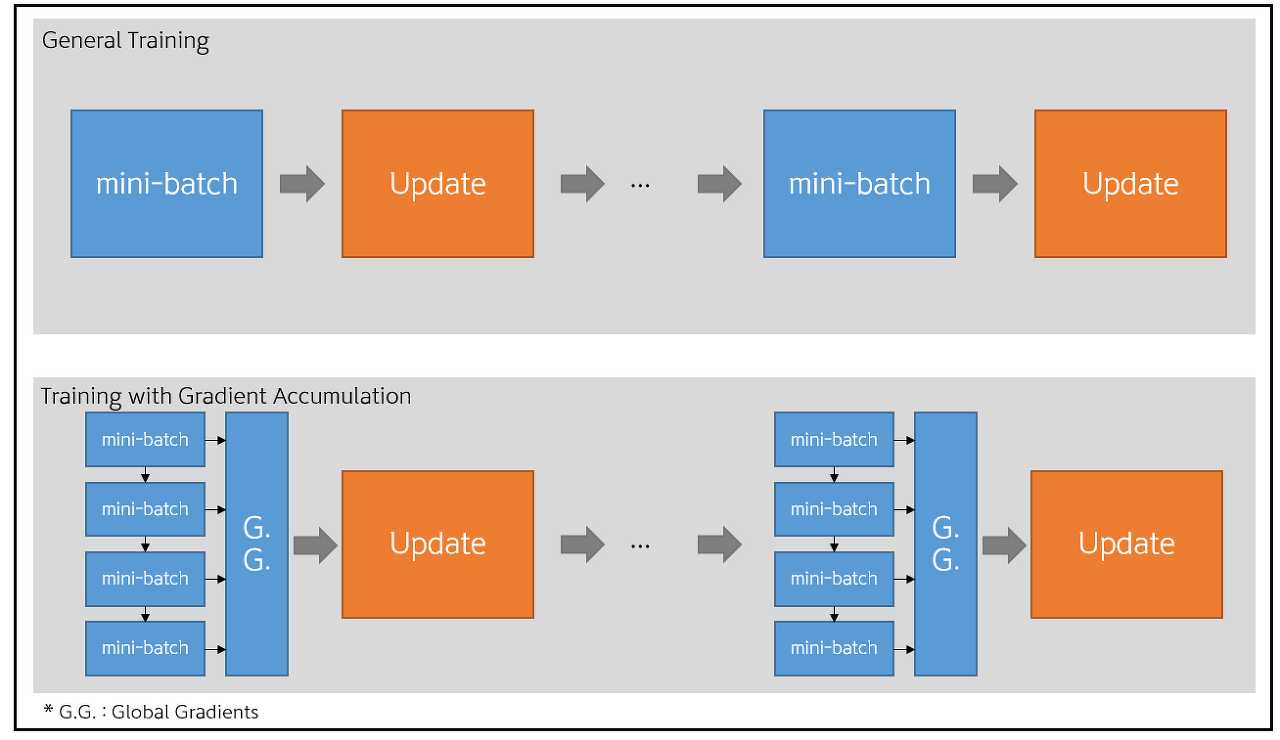
\includegraphics[width=\textwidth]{../img/proposal/gas}	
		\caption{Ejemplo de GAS. Fuente: \cite{prince2023understanding}.}		
	\end{figure}
\end{frame}
%-------------------------------------------------------
%-------------------------------------------------------

%-------------------------------------------------------
%-------------------------------------------------------
\begin{frame}{Propuesta}{\textit{Gradient Accumulation Steps}}
	\begin{figure}
		\centering
		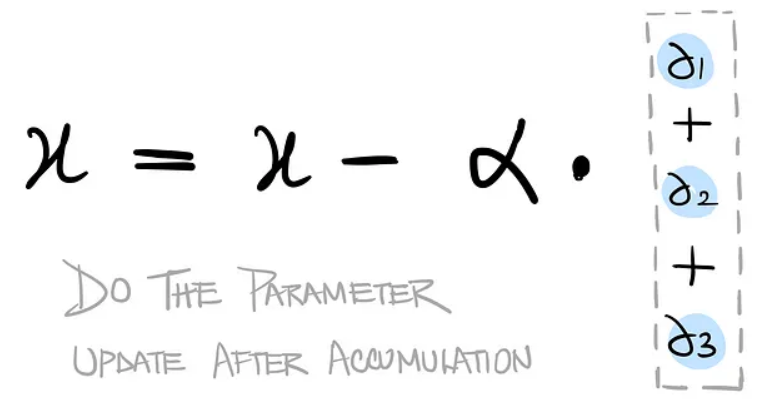
\includegraphics[width=0.6\textwidth]{../img/proposal/gas2}	
		\caption{Ejemplo de GAS. Fuente: \cite{gas2023}.}		
	\end{figure}
\end{frame}
%-------------------------------------------------------
%-------------------------------------------------------

%-------------------------------------------------------
%-------------------------------------------------------
\begin{frame}{Propuesta}{\textit{Congelamiento de capas}}
		\begin{figure}
		\centering
		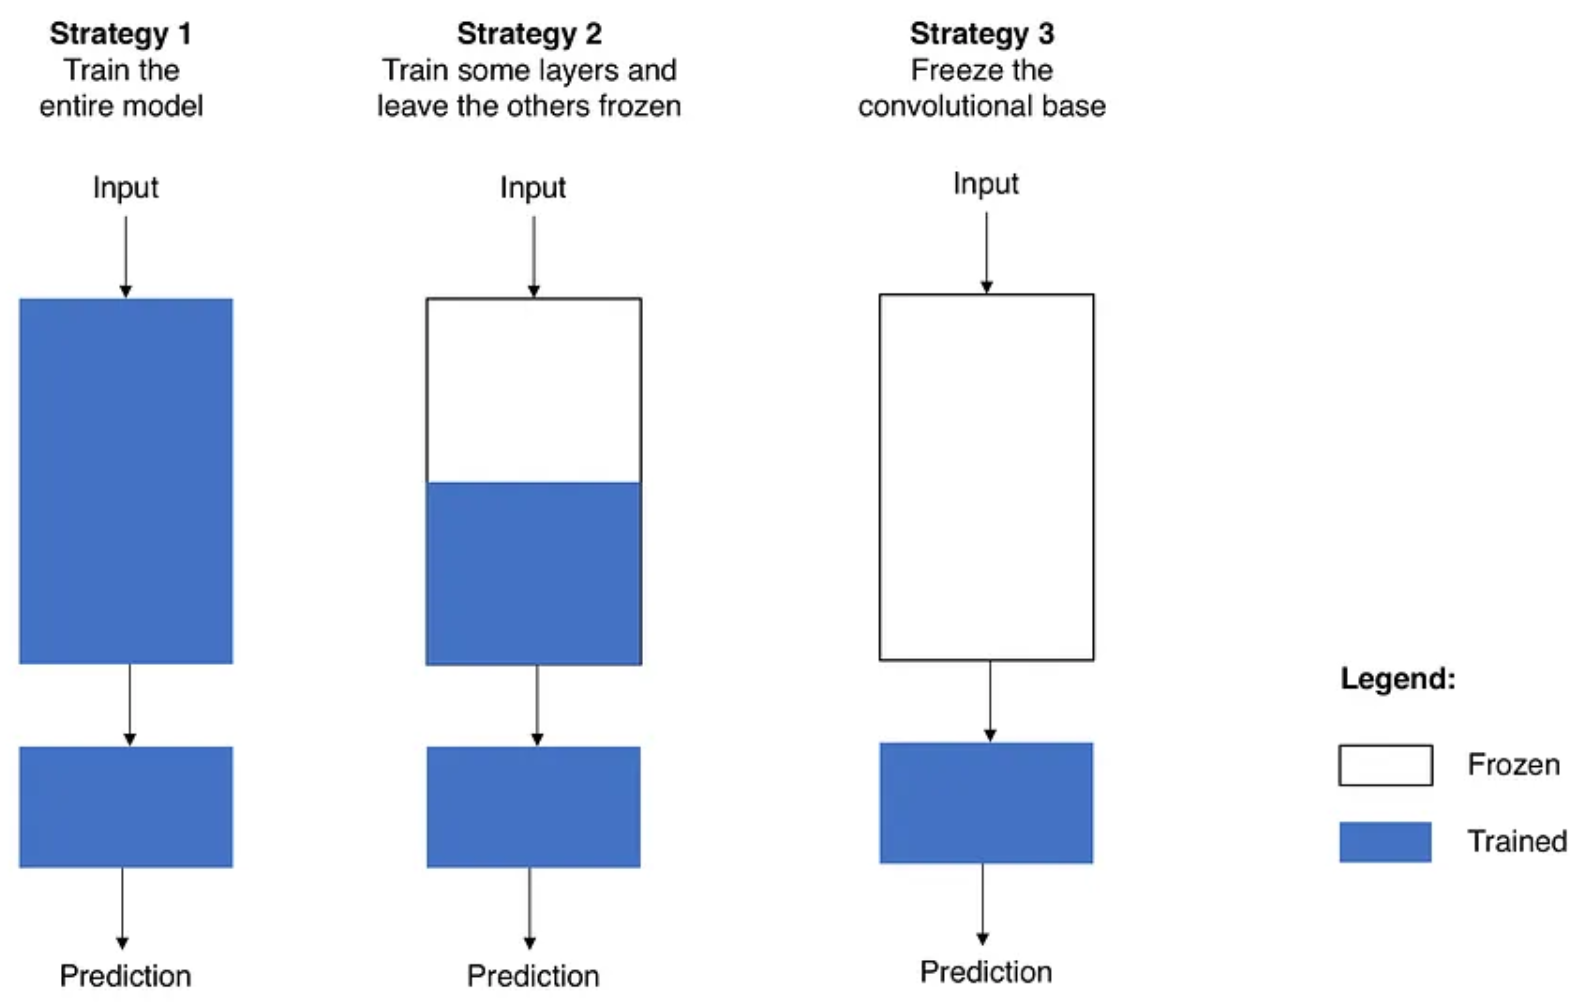
\includegraphics[width=0.9\textwidth]{../img/proposal/layer}	
		\caption{Ejemplo de congelamiento de capas. Fuente: \cite{layerf2023}.}		
	\end{figure}
\end{frame}
%-------------------------------------------------------
%-------------------------------------------------------



%%%%%%%%%%%%%%%%%%%%%%%%%%%%%%%%%%%%%%%%%%%%%%%%%%%%%%%%%%%%%%%%%%%%%%%%%%%%%%%%%%%%%%%%%%%%%%%%%%%%%%%%%%%%%%%%
%%%%%%%%%%%%%%%%%%%%%%%%%%%%%%%%%%%%%%%%%%%%%%%%%%%%%%%%%%%%%%%%%%%%%%%%%%%%%%%%%%%%%%
\section{Experimentos y Resultados}
%%%%%%%%%%%%%%%%%%%%%%%%%%%%%%%%%%%%%%%%%%%%%%%%%%%%%%%%%%%%%%%%%%%%%%%%%%%%%%%%%%%%%%%%%%%%%%%%%%%%%%%%%%%%%%%%
%%%%%%%%%%%%%%%%%%%%%%%%%%%%%%%%%%%%%%%%%%%%%%%%%%%%%%%%%%%%%%%%%%%%%%%%%%%%%%%%%%%%%%

%%%%%%%%%%%%%%%%%%%%%%%%%%%%%%%%%%%%%%%%%%%%%%%%%%%%%%%%%%%%%%%%%%%%%%%%%%%%%%%%%%%%%%%%%%%%%%%%%%%%%%%%%%%%%%%%
%%%%%%%%%%%%%%%%%%%%%%%%%%%%%%%%%%%%%%%%%%%%%%%%%%%%%%%%%%%%%%%%%%%%%%%%%%%%%%%%%%%%%%
\subsection{Base de datos}
%%%%%%%%%%%%%%%%%%%%%%%%%%%%%%%%%%%%%%%%%%%%%%%%%%%%%%%%%%%%%%%%%%%%%%%%%%%%%%%%%%%%%%%%%%%%%%%%%%%%%%%%%%%%%%%%
%%%%%%%%%%%%%%%%%%%%%%%%%%%%%%%%%%%%%%%%%%%%%%%%%%%%%%%%%%%%%%%%%%%%%%%%%%%%%%%%%%%%%%

%-------------------------------------------------------
%-------------------------------------------------------
\begin{frame}{Base de datos}{}
	
	\textit{Training}: 539,019; \textit{Validation}: 179,673; y \textit{Testing}: 172,580.
	
	\begin{figure}[]
		\centering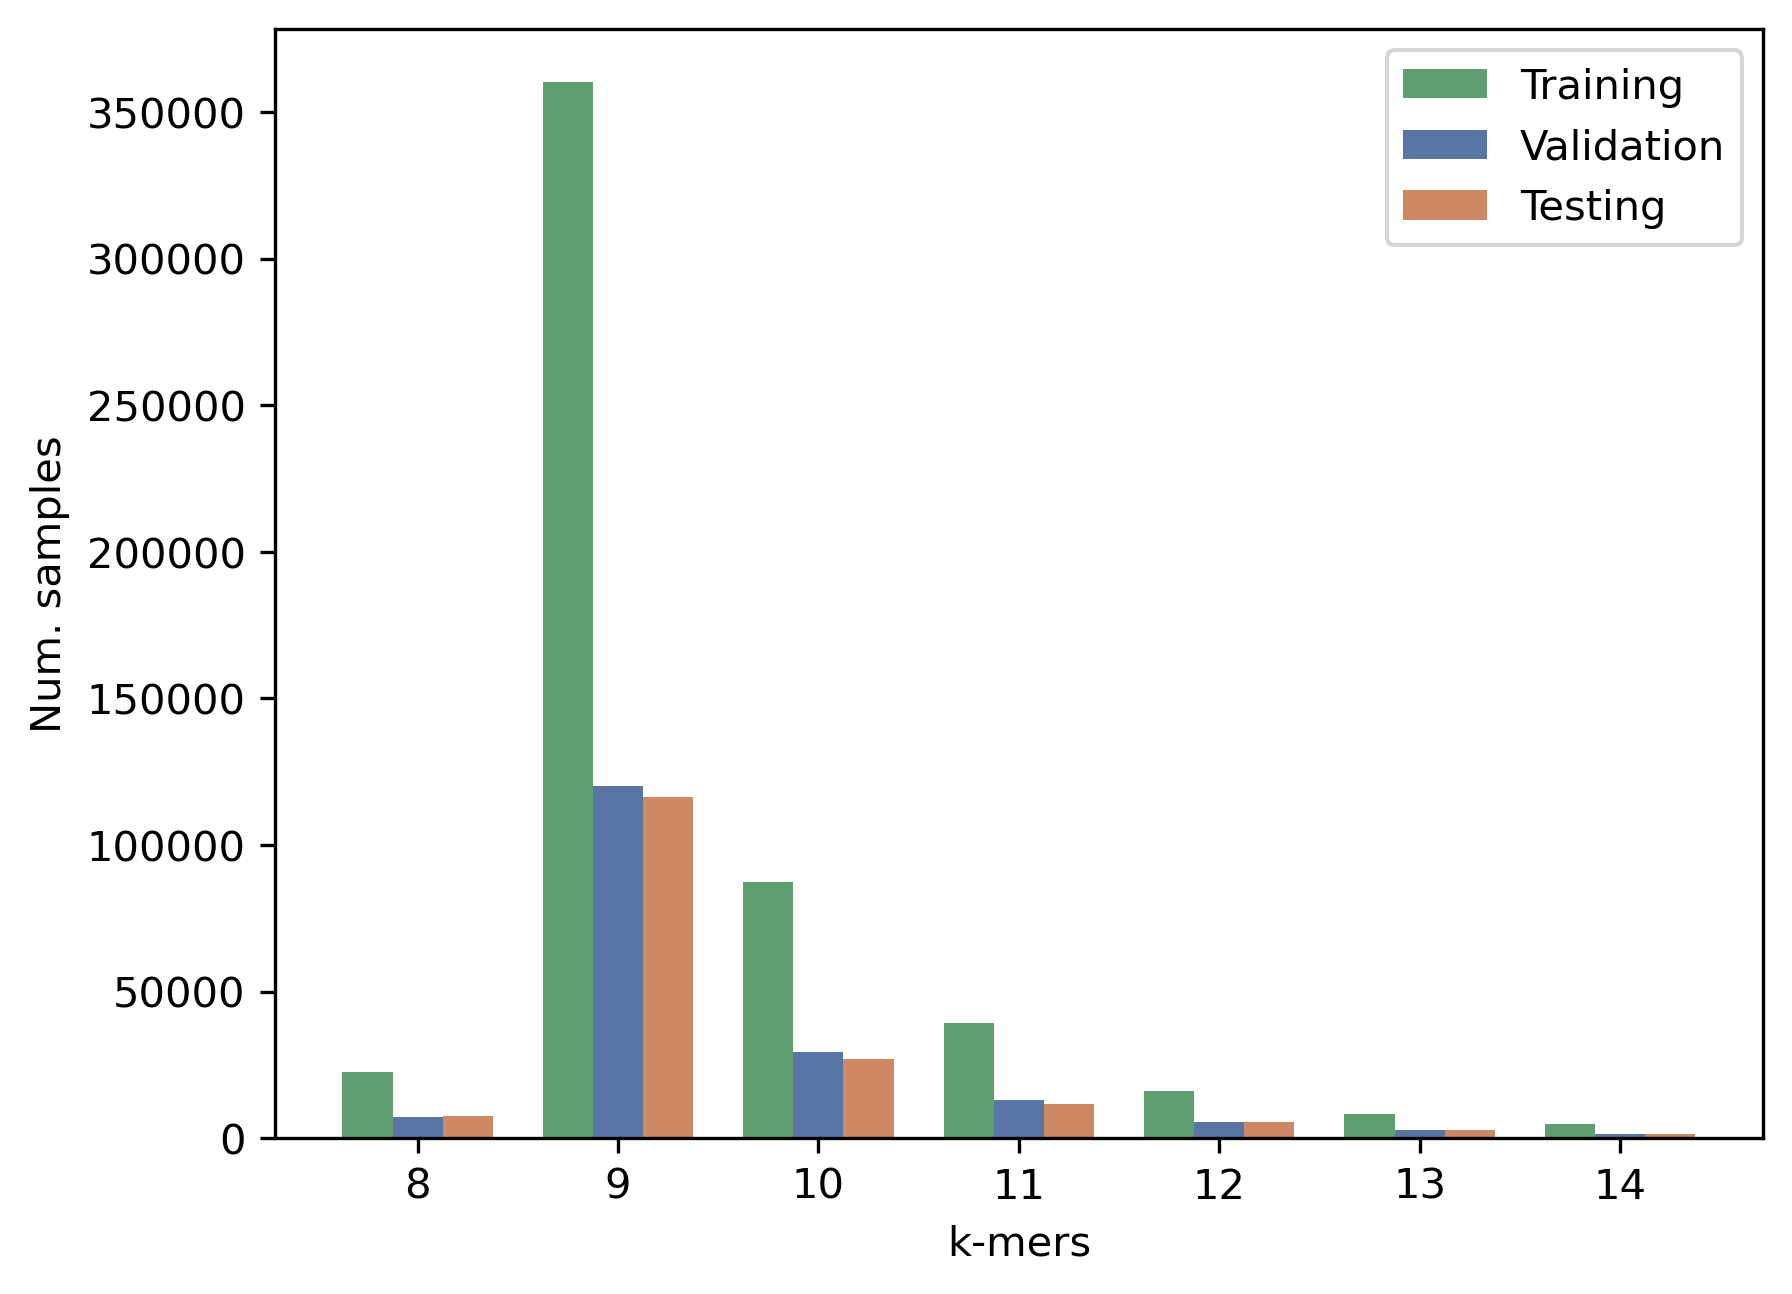
\includegraphics[width=0.7\textwidth]{../img/proposal/dataset_samples}
		\caption{
			Número de muestras por  \textit{k-mer}.}
		\label{fig:samples}
	\end{figure}
	
\end{frame}
%-------------------------------------------------------
%-------------------------------------------------------

%%%%%%%%%%%%%%%%%%%%%%%%%%%%%%%%%%%%%%%%%%%%%%%%%%%%%%%%%%%%%%%%%%%%%%%%%%%%%%%%%%%%%%%%%%%%%%%%%%%%%%%%%%%%%%%%
%%%%%%%%%%%%%%%%%%%%%%%%%%%%%%%%%%%%%%%%%%%%%%%%%%%%%%%%%%%%%%%%%%%%%%%%%%%%%%%%%%%%%%
\subsection{Modelos pre-entrenados}
%%%%%%%%%%%%%%%%%%%%%%%%%%%%%%%%%%%%%%%%%%%%%%%%%%%%%%%%%%%%%%%%%%%%%%%%%%%%%%%%%%%%%%%%%%%%%%%%%%%%%%%%%%%%%%%%
%%%%%%%%%%%%%%%%%%%%%%%%%%%%%%%%%%%%%%%%%%%%%%%%%%%%%%%%%%%%%%%%%%%%%%%%%%%%%%%%%%%%%%	

%-------------------------------------------------------
%-------------------------------------------------------
\begin{frame}{Modelos pre-entrenados}{}
	
	\begin{table}
		\centering
		\caption{Diferencias entre TAPE, ProtBert-DFB, y ESM2. HS: \textit{Hidden size}; AH: \textit{Attention heads}.}
		\label{tab:pretrained}%
		\setlength{\tabcolsep}{0.5em} % for the horizontal padding
		{\renewcommand{\arraystretch}{1.5}% for the vertical padding
			\footnotesize
			\begin{tabular}{llrrrrr}
				
				\textbf{Modelo}   & \textbf{BD} & \textbf{Muestras} & \textbf{Capas} & \textbf{HS} & \textbf{AH} & \textbf{Params.} \\
				\hline
				TAPE             & Pfam             & 30M                   & 12              & 768                  & 12                       & 92M                 \\
				ProtBert-BFD     & BFD              & 2122M                 & 30              & 1024                 & 16                       & 420M                \\
				ESM2(t6)  & Uniref50         & 60M                   & 6               & 320                  & 20                       & 8M                  \\
				ESM2(t12)  & Uniref50         & 60M                   & 12              & 480                  & 20                       & 35M                 \\
				ESM2(t30) & Uniref50         & 60M                   & 30              & 640                  & 20                       & 150M                \\
				ESM2(t33)  & Uniref50         & 60M                   & 33              & 1280                 & 20                       & 650M               \\
				
		\end{tabular}}
		
	\end{table}
	
\end{frame}
%-------------------------------------------------------
%-------------------------------------------------------


%%%%%%%%%%%%%%%%%%%%%%%%%%%%%%%%%%%%%%%%%%%%%%%%%%%%%%%%%%%%%%%%%%%%%%%%%%%%%%%%%%%%%%%%%%%%%%%%%%%%%%%%%%%%%%%%
%%%%%%%%%%%%%%%%%%%%%%%%%%%%%%%%%%%%%%%%%%%%%%%%%%%%%%%%%%%%%%%%%%%%%%%%%%%%%%%%%%%%%%
\subsection{Resultados}
%%%%%%%%%%%%%%%%%%%%%%%%%%%%%%%%%%%%%%%%%%%%%%%%%%%%%%%%%%%%%%%%%%%%%%%%%%%%%%%%%%%%%%%%%%%%%%%%%%%%%%%%%%%%%%%%
%%%%%%%%%%%%%%%%%%%%%%%%%%%%%%%%%%%%%%%%%%%%%%%%%%%%%%%%%%%%%%%%%%%%%%%%%%%%%%%%%%%%%%	

%-------------------------------------------------------
%-------------------------------------------------------
\begin{frame}{Resultados}{Entrenamiento por 3 \textit{epochs}}
	\begin{figure}
		\centering		
		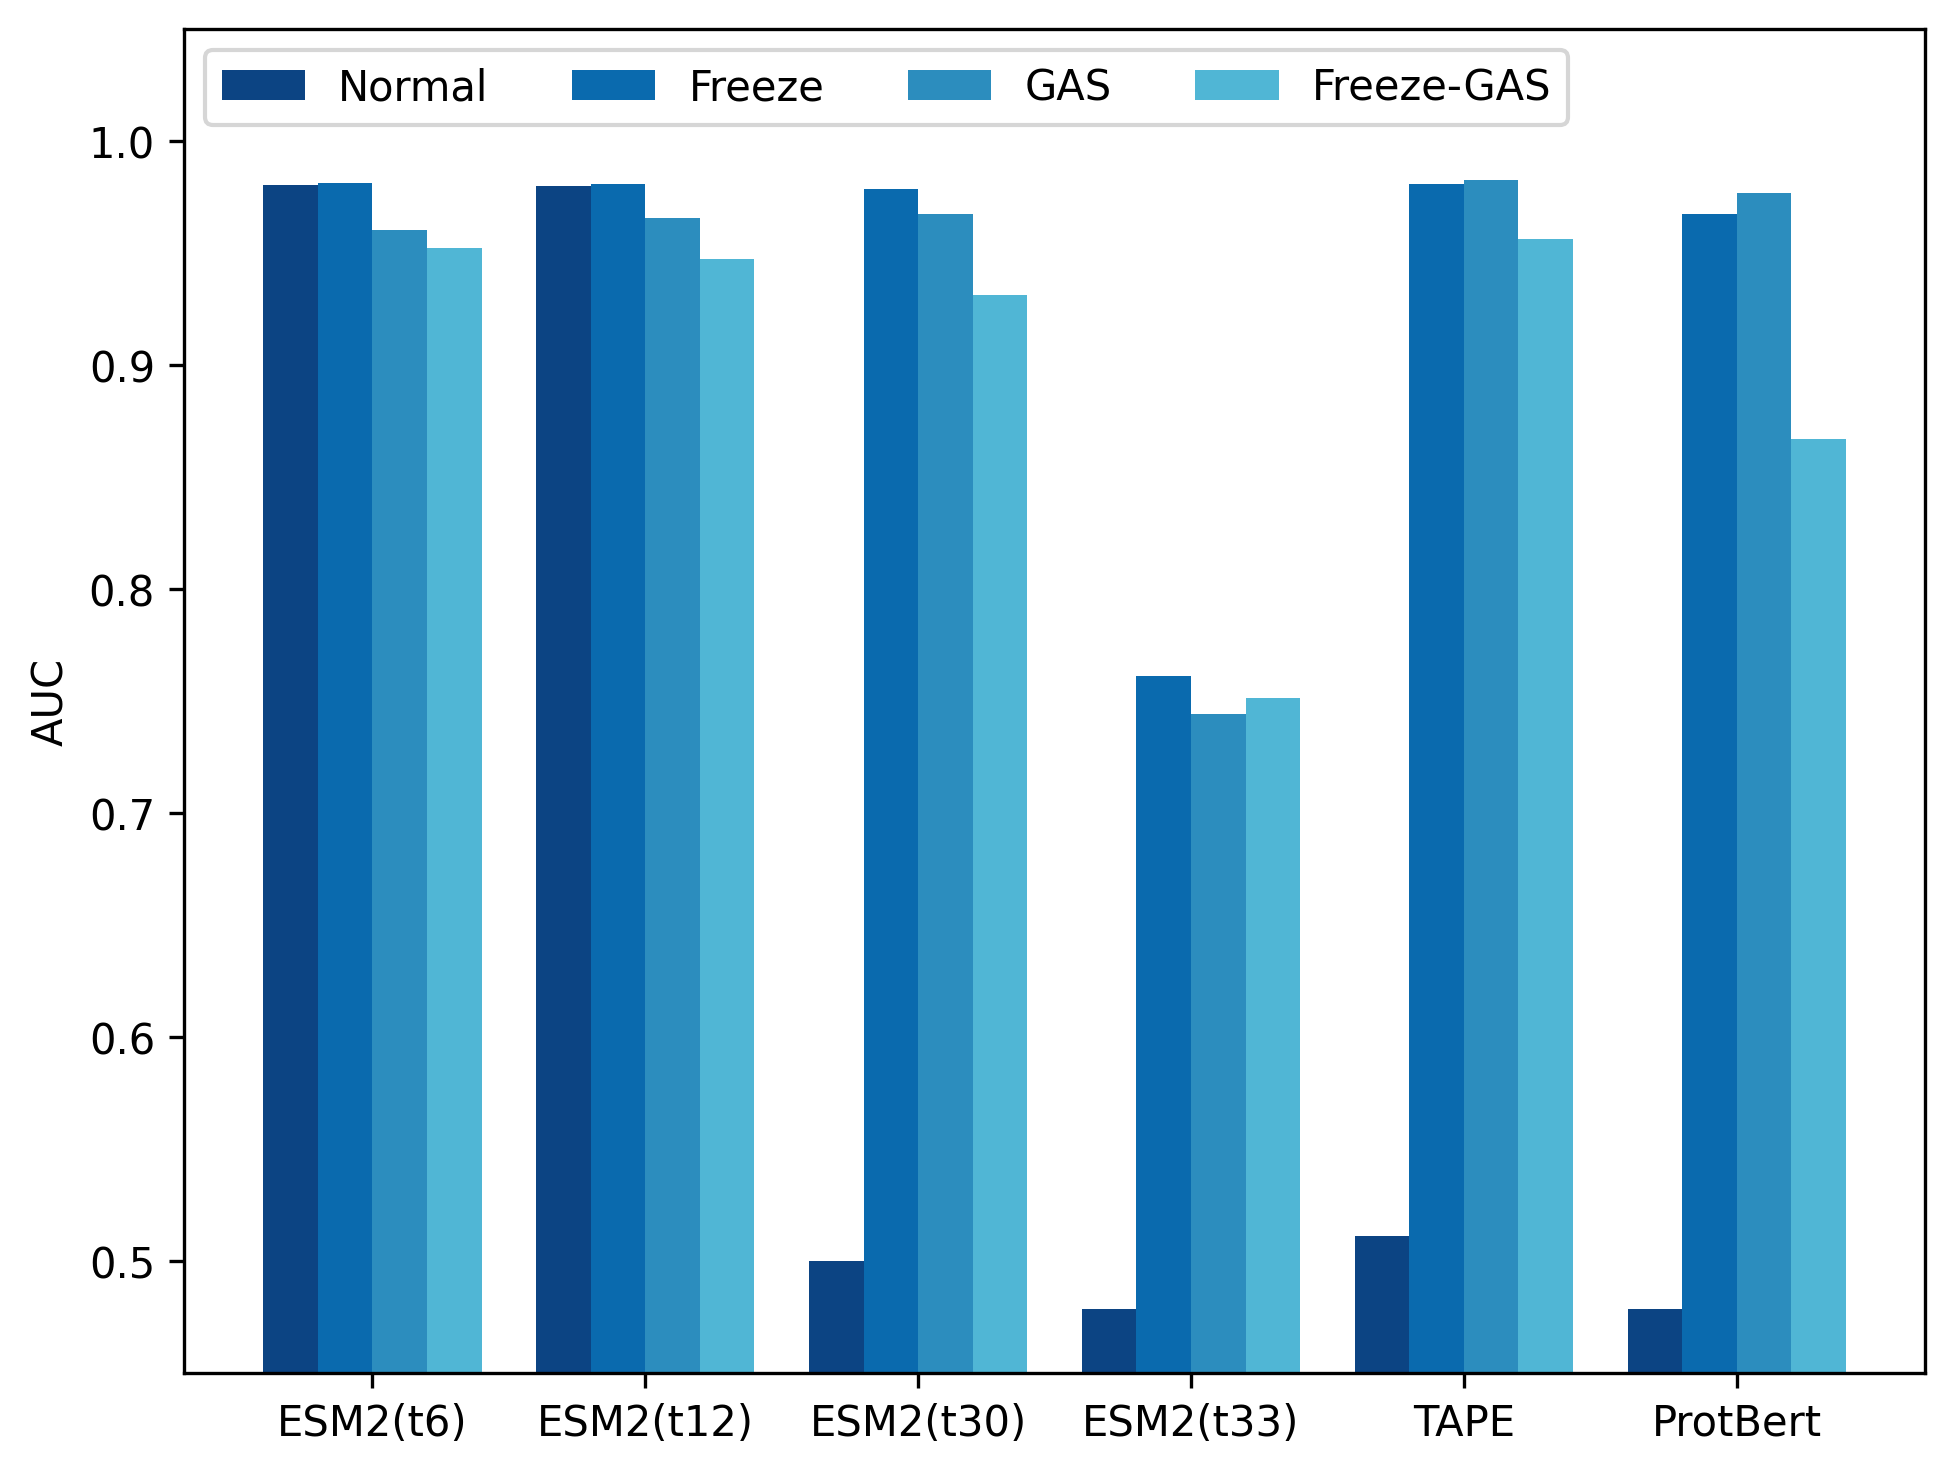
\includegraphics[width=0.7\textwidth]{../img/results/metrics_comparion_by_model.png}			
		\caption{Comparación del AUC por modelo y metodología de entrenamiento.}
	\end{figure}
\end{frame}
%-------------------------------------------------------
%-------------------------------------------------------


%-------------------------------------------------------
%-------------------------------------------------------
\begin{frame}{Resultados}{Problema de \textit{vanish gradient} para ESM2(t6)}
	\centering
	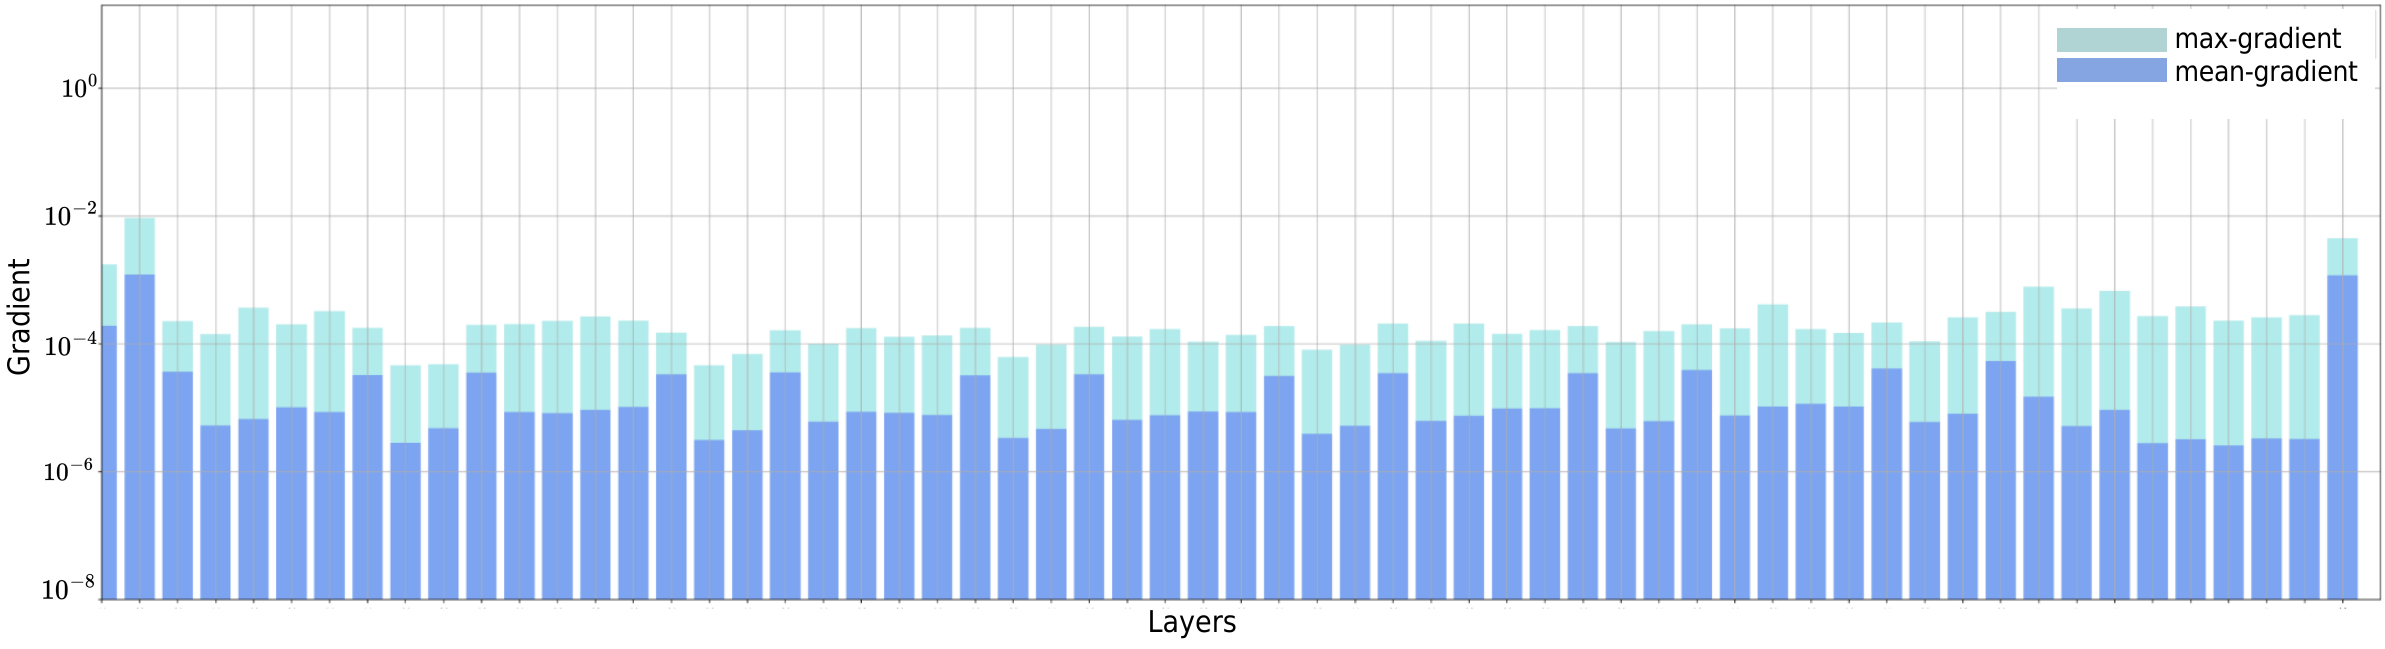
\includegraphics[width=\textwidth]{../img/results/t6_epoch0}
	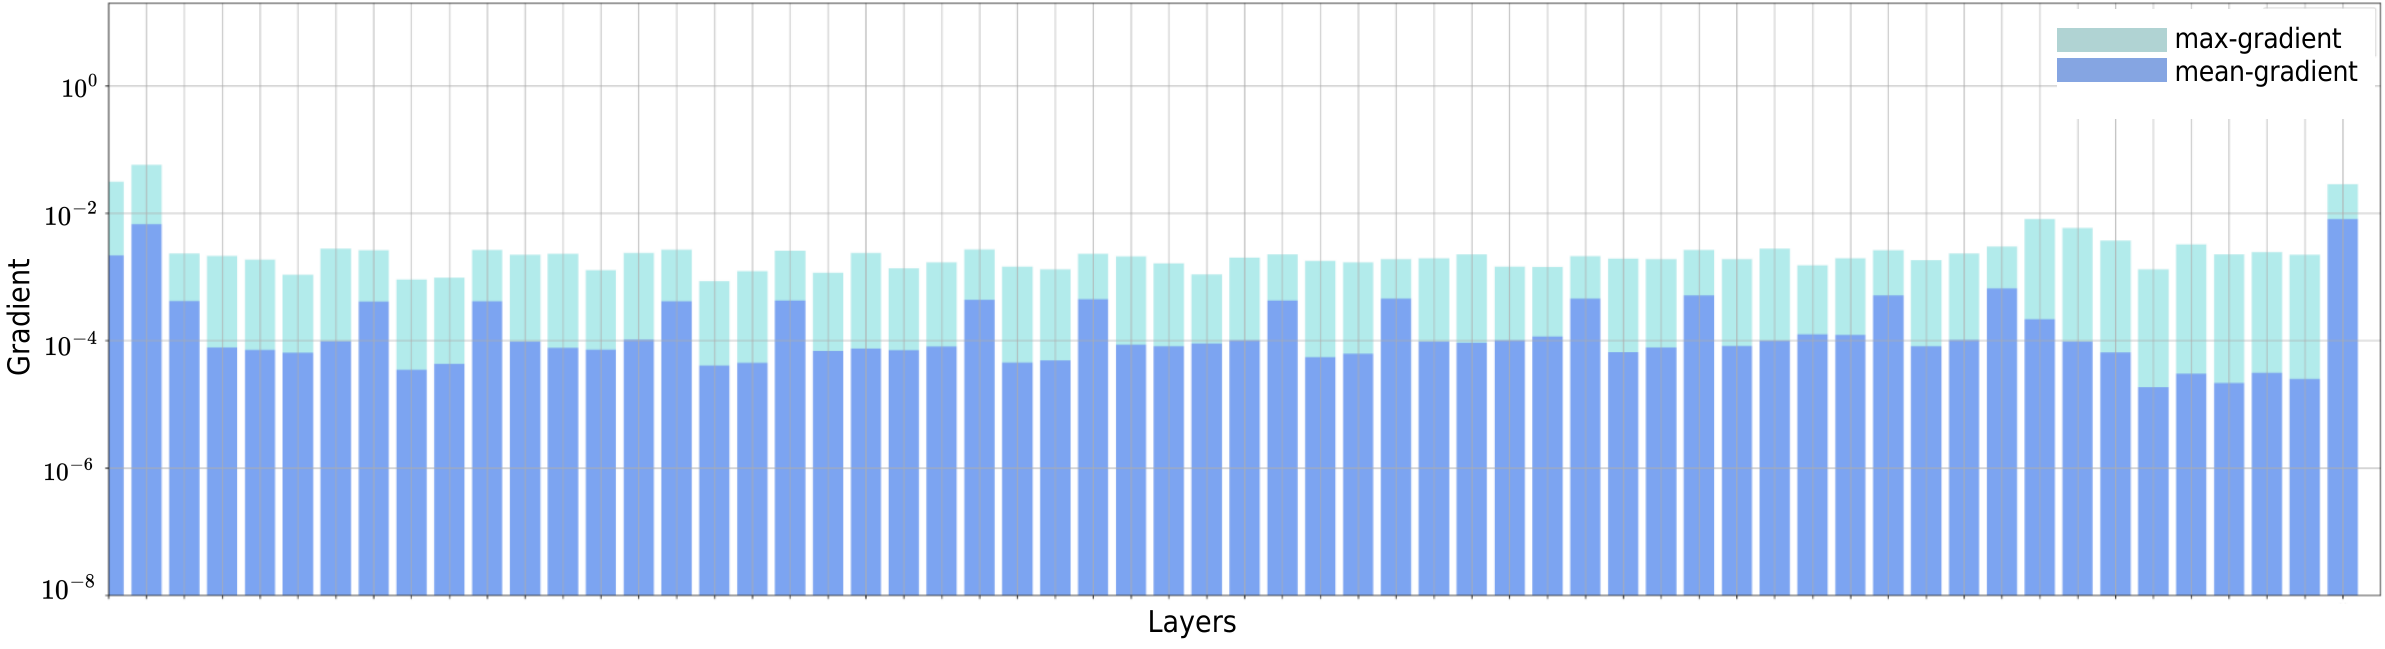
\includegraphics[width=\textwidth]{../img/results/t6_epoch3}
\end{frame}
%-------------------------------------------------------
%-------------------------------------------------------

%-------------------------------------------------------
%-------------------------------------------------------
\begin{frame}{Resultados}{Problema de \textit{vanish gradient} para ESM2(t30)}
	\centering

	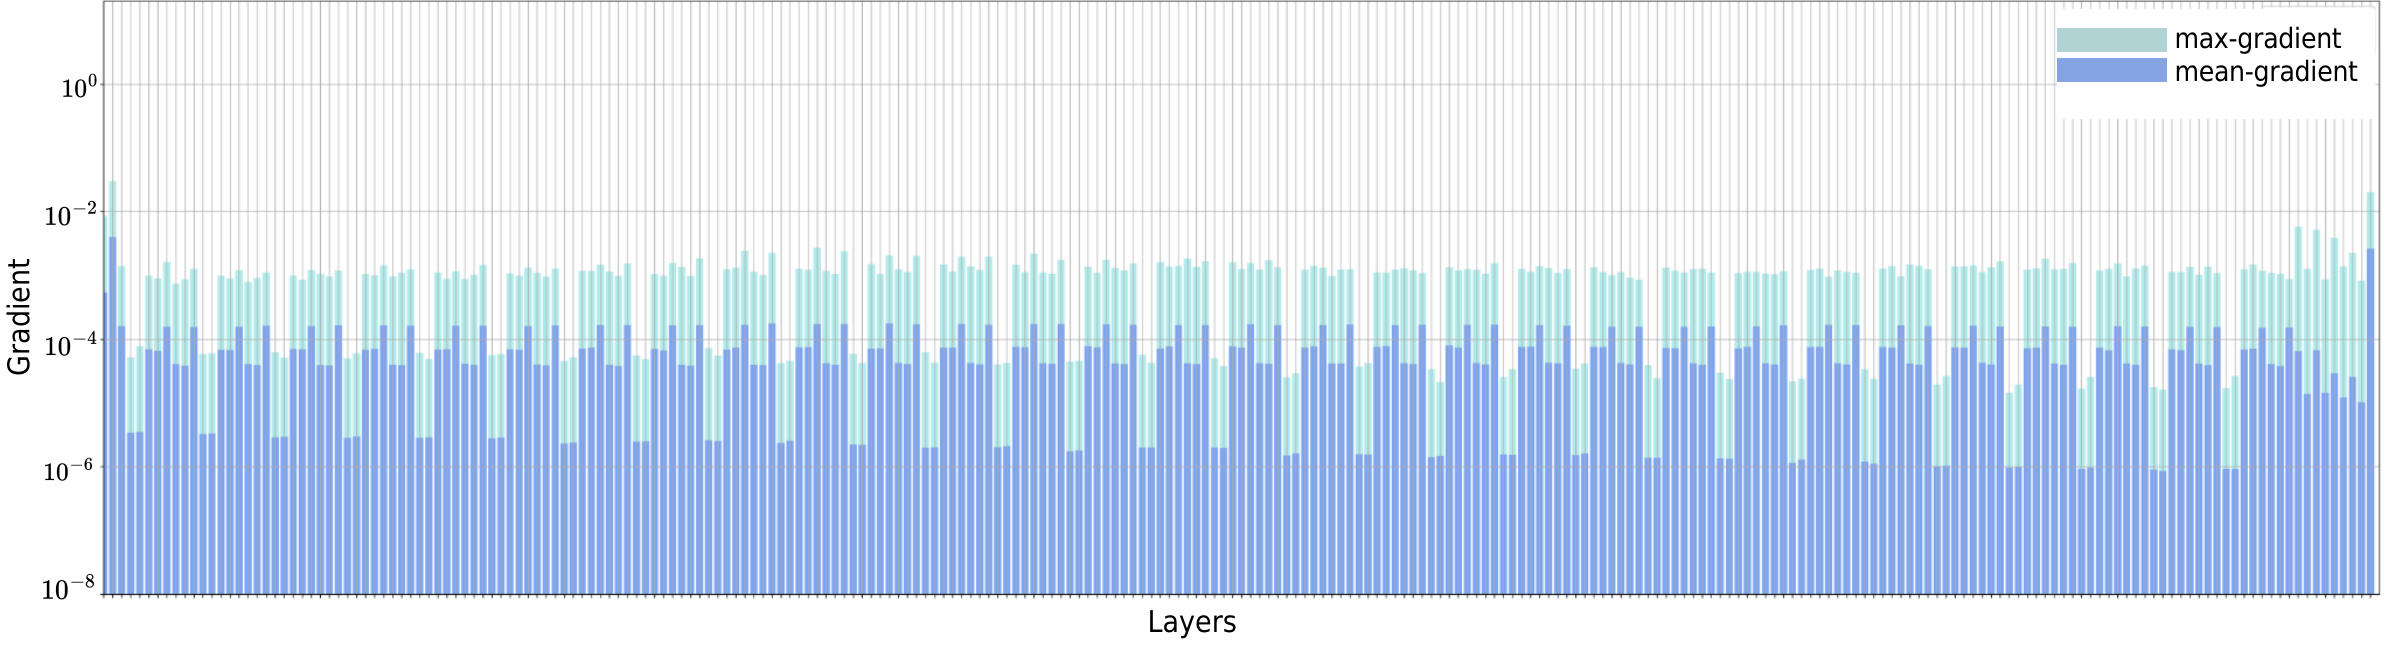
\includegraphics[width=\textwidth]{../img/results/t30_epoch0}
	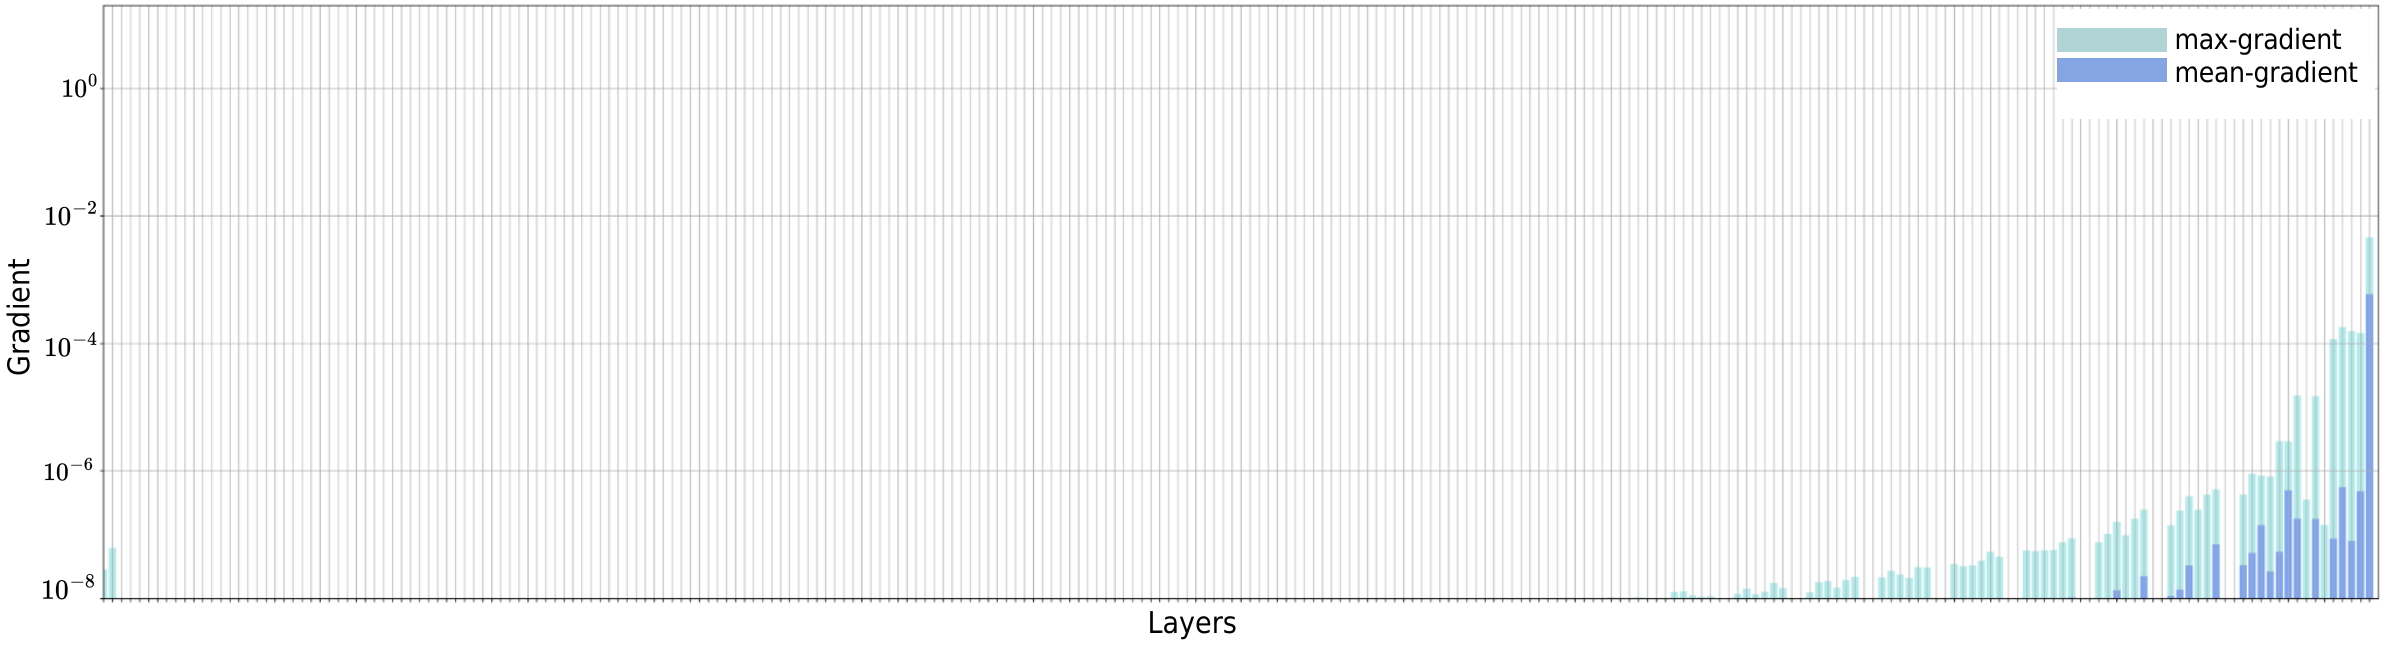
\includegraphics[width=\textwidth]{../img/results/t30_epoch3}
\end{frame}
%-------------------------------------------------------
%-------------------------------------------------------

%-------------------------------------------------------
%-------------------------------------------------------
\begin{frame}{Resultados}{Entrenamiento por 30 \textit{epochs}}
	\begin{table}[]
		\centering
		\setlength{\tabcolsep}{0.5em} % for the horizontal padding
		{\renewcommand{\arraystretch}{1.5}% for the vertical padding
			\scriptsize
			\begin{tabular}{lllllll} 
				\textbf{}            & \textbf{Accuracy} & \textbf{Precision} & \textbf{Recall} & \textbf{F1-score} & \textbf{AUC}    & \textbf{MCC}    \\ \hline
				ESM2(t6)-Normal             & 0.9390            & 0.9333             & \textbf{0.9453} & 0.9392            & 0.9797          & 0.8780                    \\
				ESM2(t6)-Freeze      & \textbf{0.9401}   & \textbf{0.9398}    & 0.9402          & \textbf{0.9400}   & \textbf{0.9830} & \textbf{0.8802}             \\
				ESM2(t6)-GAS         & 0.9366            & 0.9322             & 0.9413          & 0.9368            & 0.9818          & 0.8732                     \\
				ESM2(t6)-Freeze-GAS  & 0.9354            & 0.9326             & 0.9383          & 0.9355            & 0.9813          & 0.8708                    \\ \hline
				ESM2(t30)-Normal            & -                 & -                  & -               & -                 & -               & -                                 \\
				ESM2(t30)-Freeze     & \textbf{0.9393}   & 0.9304             & \textbf{0.9493} & \textbf{0.9397}   & 0.9787          & \textbf{0.8787}           \\
				ESM2(t30)-GAS        & 0.9346            & \textbf{0.9337}    & 0.9352          & 0.9345            & 0.9808          & 0.8691                    \\
				ESM2(t30)-Freeze-GAS & 0.9363            & 0.9319             & 0.9411          & 0.9365            & \textbf{0.9818} & 0.8726                    \\ \hline
				TAPE-Normal                 & -                 & -                  & -               & -                 & -               & -                                  \\
				TAPE-Freeze          & 0.9395            & \textbf{0.9404}    & 0.9382          & 0.9393            & 0.9815          & 0.8790                      \\
				TAPE-GAS             & \textbf{0.9415}   & 0.9352             & \textbf{0.9484} & \textbf{0.9418}   & \textbf{0.9841} & \textbf{0.8831}            \\
				TAPE-Freeze-GAS      & 0.9359            & 0.9297             & 0.9428          & 0.9362            & 0.9820          & 0.8719               \\     
		\end{tabular}}
	\end{table}
\end{frame}
%-------------------------------------------------------
%-------------------------------------------------------


%-------------------------------------------------------
%-------------------------------------------------------
\begin{frame}{Resultados}{Comparación con los métodos \textit{state-of-art}}
	\begin{figure}
		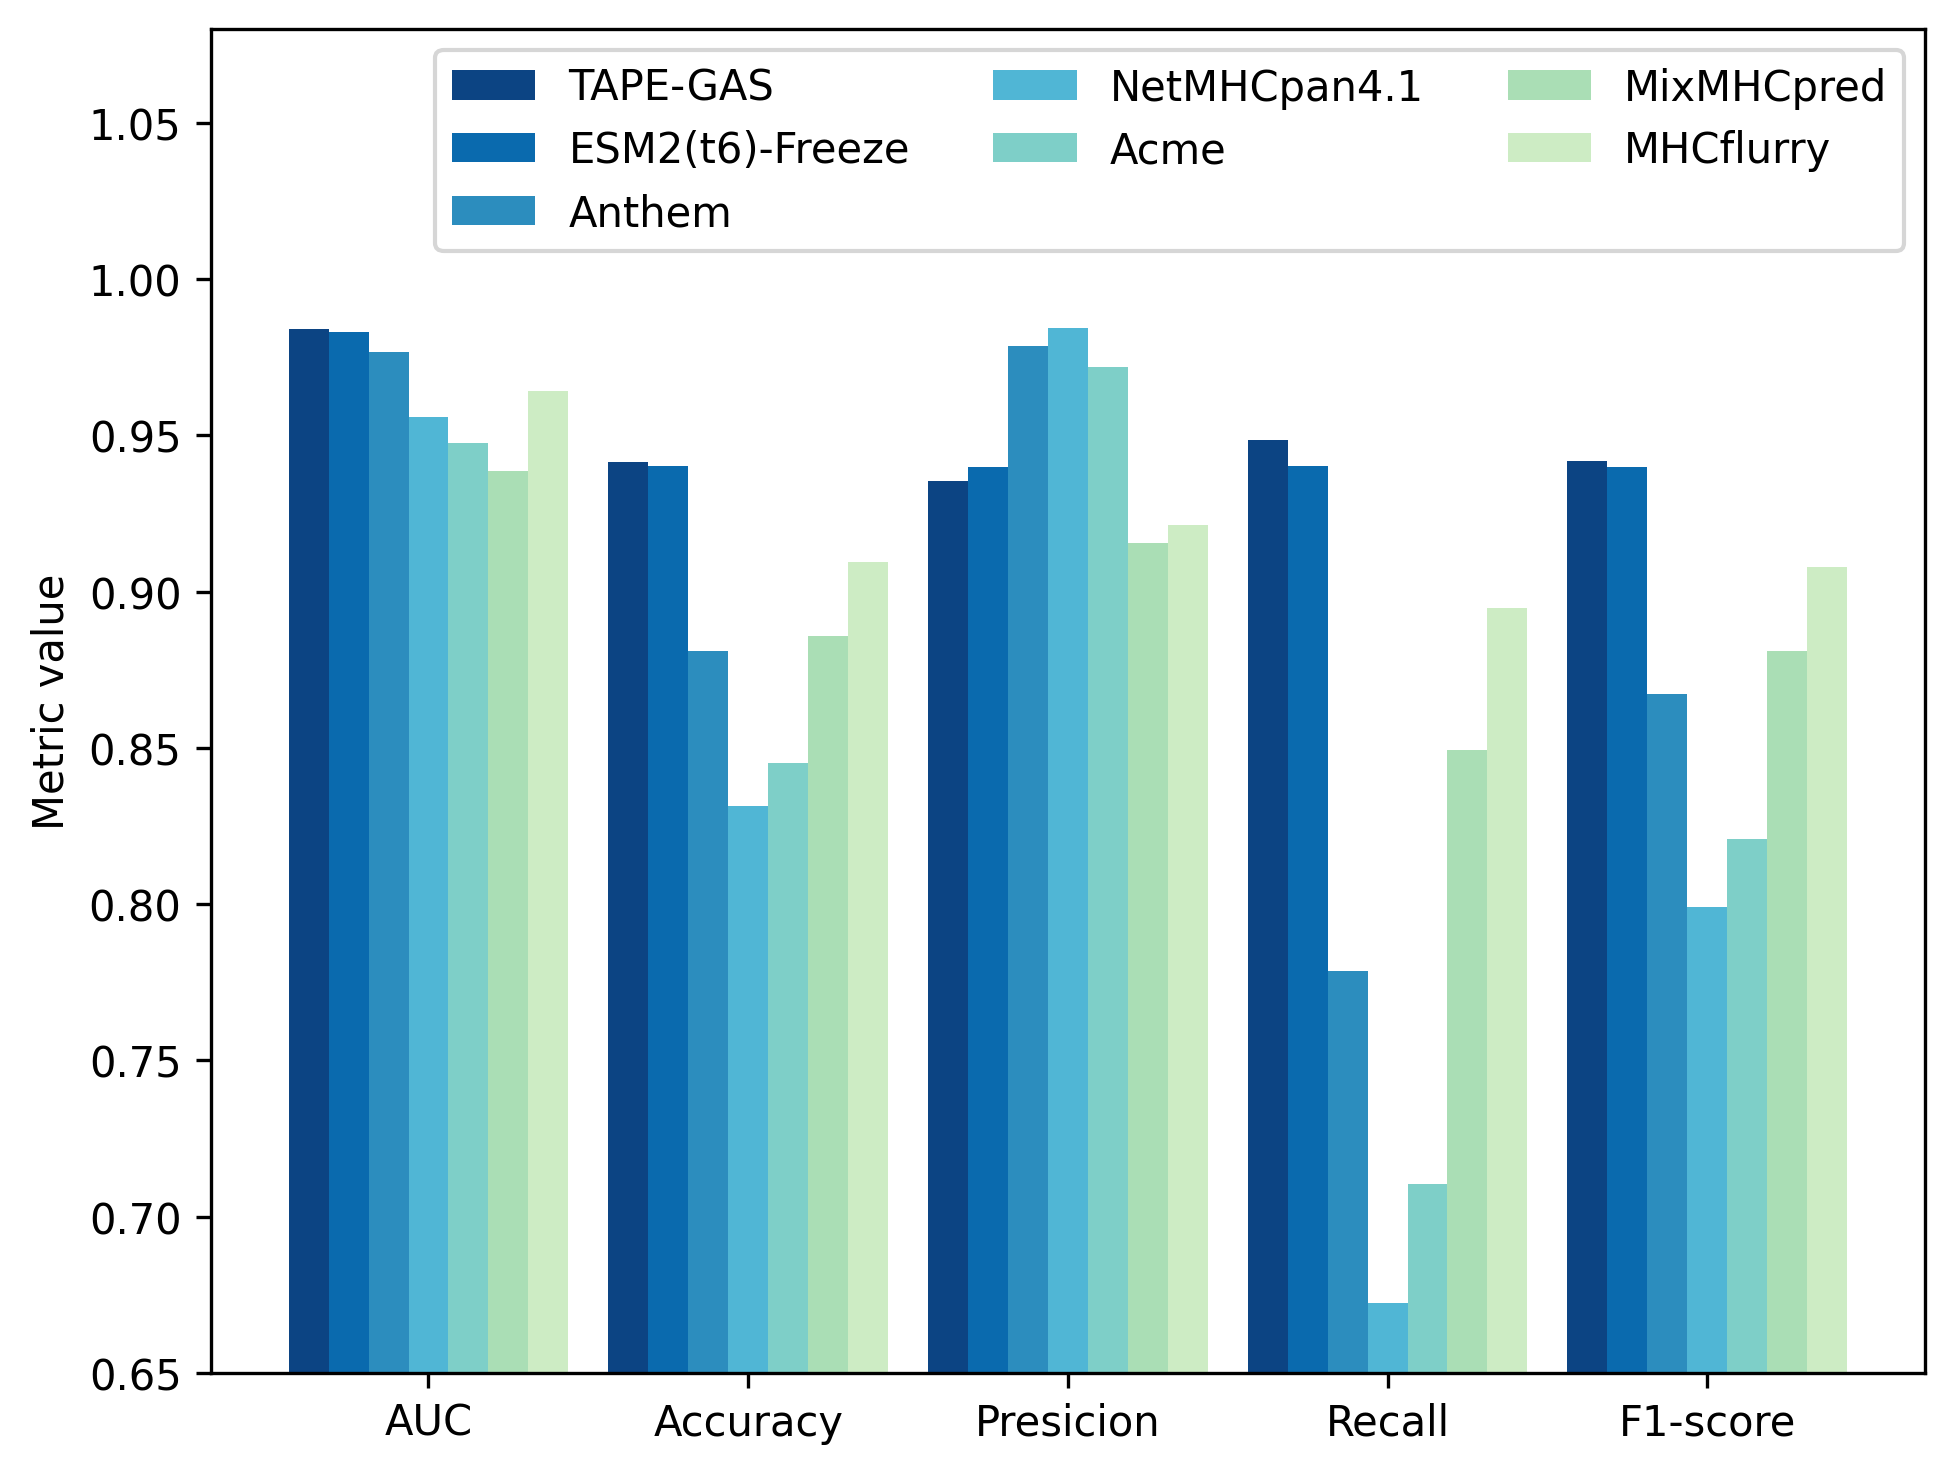
\includegraphics[width=0.75\textwidth]{../img/results/metrics_comparison}
		\caption{Comparación de TAPE-GAS y ESM2(t6) contra los mejores métodos del estado del arte.}
	\end{figure}
\end{frame}
%-------------------------------------------------------
%-------------------------------------------------------

%-------------------------------------------------------
%-------------------------------------------------------
\begin{frame}{Resultados}{Comparación con los métodos \textit{state-of-art}}
	\begin{figure}
		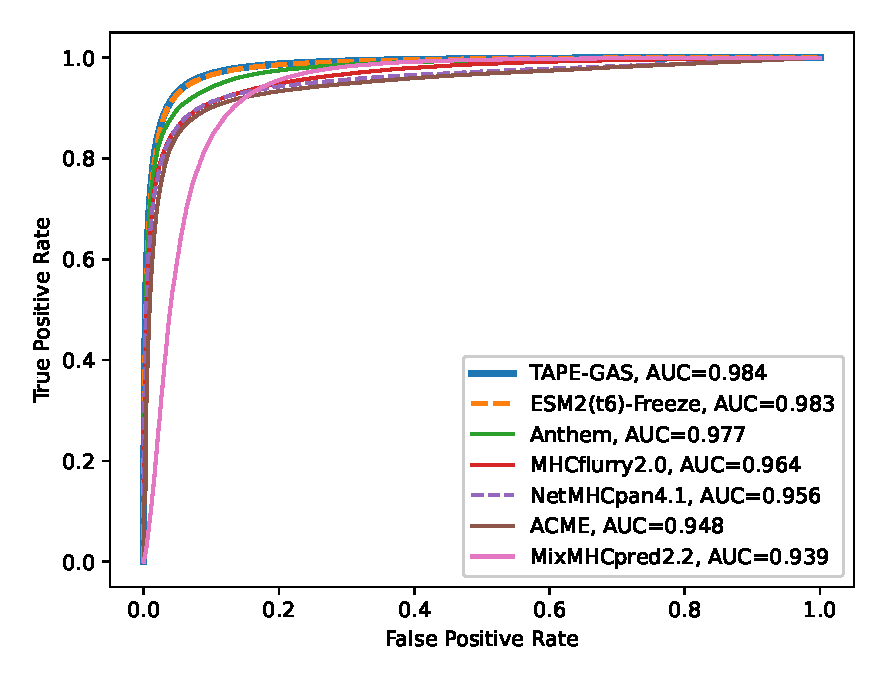
\includegraphics[width=0.75\textwidth]{../img/results/ROC_comparison}
		\caption{Comparación de TAPE-GAS y ESM2(t6) contra los mejores métodos del estado del arte.}
	\end{figure}
\end{frame}
%-------------------------------------------------------
%-------------------------------------------------------

%-------------------------------------------------------
%-------------------------------------------------------
\begin{frame}{Resultados}{Comparación con los métodos \textit{state-of-art}}
	\begin{table}[]
		\centering
		\caption{Desempeño de TAPE-GAS y ESM2(t6)-Freeze, entrenados por 30 \textit{epochs}, contra Anthem, NetMHCpan4.1, ACME, MixMHCpred2.2, y MhcFlurry2.0.}
		\setlength{\tabcolsep}{0.5em} % for the horizontal padding
		{\renewcommand{\arraystretch}{1.5}% for the vertical padding
			\scriptsize
			\begin{tabular}{lllllll} 
				& \textbf{Accuracy} & \textbf{Precision} & \textbf{Recall} & \textbf{F1-score} & \textbf{AUC}    & \textbf{MCC}    \\ \hline
				TAPE-GAS        & \textbf{0.9415}   & 0.9352             & \textbf{0.9484} & \textbf{0.9418}   & \textbf{0.9841} & \textbf{0.8831} \\
				ESM2(t6)-Freeze & \textbf{0.9401}   & 0.9398             & \textbf{0.9402} & \textbf{0.9400}   & \textbf{0.9830} & \textbf{0.8802} \\
				
				Anthem          & 0.8811            & \textbf{0.9786}    & 0.7787          & 0.8673            & 0.9768          & 0.7785          \\
				NetMHCpan4.1    & 0.8312            & \textbf{0.9844}    & 0.6724          & 0.7991            & 0.9557          & 0.6982          \\
				
				ACME            & 0.8452            & 0.9717             & 0.7105          & 0.8208            & 0.9476          & 0.7165          \\
				MixMHCpred2.2   & 0.8857            & 0.9155             & 0.8493          & 0.8811            & 0.9386          & 0.7733          \\
				MhcFlurry2.0    & 0.9093            & 0.9211             & 0.8948          & 0.9078            & 0.9642          & 0.8189 \\         
		\end{tabular}}
	\end{table}
\end{frame}
%-------------------------------------------------------
%-------------------------------------------------------


%%%%%%%%%%%%%%%%%%%%%%%%%%%%%%%%%%%%%%%%%%%%%%%%%%%%%%%%%%%%%%%%%%%%%%%%%%%%%%%%%%%%%%%%%%%%%%%%%%%%%%%%%%%%%%%%
%%%%%%%%%%%%%%%%%%%%%%%%%%%%%%%%%%%%%%%%%%%%%%%%%%%%%%%%%%%%%%%%%%%%%%%%%%%%%%%%%%%%%%
\section{Discusión}
%%%%%%%%%%%%%%%%%%%%%%%%%%%%%%%%%%%%%%%%%%%%%%%%%%%%%%%%%%%%%%%%%%%%%%%%%%%%%%%%%%%%%%%%%%%%%%%%%%%%%%%%%%%%%%%%
%%%%%%%%%%%%%%%%%%%%%%%%%%%%%%%%%%%%%%%%%%%%%%%%%%%%%%%%%%%%%%%%%%%%%%%%%%%%%%%%%%%%%%




%-------------------------------------------------------
%-------------------------------------------------------
\begin{frame}{Discusión}{¿Porque el modelo mas pequeño de la familia ESM2 es el mejor?}
	
	\begin{block}{}
		El modelo más pequeño, ESM2(t6) supero a los demás. Las causas de este fenómeno pueden ser: 
	
	\end{block}
	
	\pause
	
	\begin{block}{}
		\begin{itemize}
			\item En conjunto de datos que consta de 559,019 muestras, que no consideramos lo suficientemente grande para ESM2(t33), un modelo que cuenta con 650 millones de parámetros. \pause
			
			\item El uso de \textit{Rotary Position Embedding} (RoPE) en lugar de la codificación posicional absoluta. Si bien RoPE puede llevar a un ligero aumento en el costo de entrenamiento, se ha observado que mejora la calidad de los resultados, especialmente para modelos más pequeños \cite{lin2023evolutionary}.
		\end{itemize}
	\end{block}
	
\end{frame}
%-------------------------------------------------------
%-------------------------------------------------------

%-------------------------------------------------------
%-------------------------------------------------------
%\begin{frame}{Discusión}{Congelamiento de capas y GAS}
	
	
%	\begin{block}{Congelamiento de capas}
%	Para los modelos ESM2, esta metodología arrojó los mejores resultados, mientras que para TAPE y ProtBert-BFD, produjo los resultados esperados
%	\end{block}

%\pause
	
%	\begin{block}{GAS}
%	Esta técnica alivia ligeramente el problema de \textit{vanish gradients} acumulando las gradientes durante las iteraciones. En si, este técnica extiende la cantidad de iteraciones de entrenamiento que se pueden realizar antes de que el modelo posiblemente vuelva a enfrentar el problema de \textit{vanish gradient}.
%	\end{block}
%\end{frame}
%-------------------------------------------------------
%-------------------------------------------------------


%-------------------------------------------------------
%-------------------------------------------------------
\begin{frame}{Discusión}{TAPE, ProtBert-BFD y ESM2}
	
	\begin{block}{ProtBert-BFD}
		ProtBert-BFD (420M parámetros) obtuvo el peor resultado a pesar de que este modelo fue \textbf{pre-entrenado con el conjunto de datos más grande (2122 millones de muestras)}. Las causas son: 
	\end{block}

	\begin{block}{}
		\begin{itemize}
			\item  Ruido en las muestras y a los errores en las secuencias en el conjunto de datos BFD \cite{elnaggar2021prottrans}.
			%\item Los modelos \textit{Transformer} grandes requieren más datos para el entrenamiento \cite{elnaggar2021prottrans}, y en nuestro caso este modelo se entreno con 559,019 muestras.
		\end{itemize}
	\end{block}
	
\end{frame}
%-------------------------------------------------------
%-------------------------------------------------------



%-------------------------------------------------------
%-------------------------------------------------------
\begin{frame}{Discusión}{TAPE, ProtBert-BFD y ESM2}
	
	\begin{block}{TAPE}
		TAPE logró los mejores resultados. Este solo fue pre-entrenado con 30 millones de muestras; sin embargo, secuencias pertenecen a \textit{Reference Proteomes} en lugar de abarcar toda la base de datos de UniProtKB \cite{finn2016pfam}. 
	\end{block}
	
	\begin{block}{ESM2}
		ESM2(t6) logró resultados que compiten estrechamente con el desempeño de TAPE; sin embargo ESM2(t6) tiene 8M contra los 92M de parámetros de TAPE.		
	\end{block}
\end{frame}
%-------------------------------------------------------
%-------------------------------------------------------


\section{Conclusiones}

%-------------------------------------------------------
%-------------------------------------------------------
\begin{frame}{Conclusiones}{PRIMERA}
	
	\begin{block}{PRIMERA}
		Se revisó y analizó los métodos que utilizan \textit{Transformers} para la predicción del enlace pMHC.  Este análisis ha demostrado que existen varios problemas como: 
		\pause
		\begin{itemize}
			\item No inclusión de datos de MS.\pause
			\item Bajo rendimiento en las herramientas de predicción pMHC y pMHC-TCR.\pause
			\item Falta de métodos para la detección de fusión de genes y \textit{alternative splicing}.
		\end{itemize}

	\pause
		\textbf{Sin embargo, a pesar de estas limitaciones, ya se han realizado ensayos clínicos con resultados motivadores.}
	\end{block}
	
	
\end{frame}
%-------------------------------------------------------
%-------------------------------------------------------

%-------------------------------------------------------
%-------------------------------------------------------
\begin{frame}{Conclusiones}{SEGUNDA}	
	\begin{block}{SEGUNDA}
		Se analizó los modelos \textit{Transformers} pre-entrenados como: TAPE, ProtBert-BFD, y la familia de modelos de EMS2, para tareas de Proteómica.
			\pause
		
		\begin{itemize}
			\item ProtBert-BFD fue entrenado con la base de datos mas grande proteínas (2122M). \pause
			\item TAPE se entreno con la base de datos mas pequeña (30M). \pause
			\item Familia de modelos ESM2, recientemente publicada (60M). 
		\end{itemize}	
	
	\end{block}	
\end{frame}
%-------------------------------------------------------
%-------------------------------------------------------

%-------------------------------------------------------
%-------------------------------------------------------
\begin{frame}{Conclusiones}{TERCERA}	
	\begin{block}{TERCERA}
		Se aplicó \textit{fine-tuning} a los seis modelos pre-entrenados agregando un bloque BiLSTM. Adicionalmente, se evaluó el uso de GAS y una metodología congelamiento de capas. \pause
		\begin{itemize}
			\item Los modelos ESM2 mejoran al aplicar el congelamiento de capas. \pause
			\item GAS ofreció una mitigación menor del problema de \textit{vanish gradientes}, lo que permitió el entrenamiento efectivo de modelos más grandes.
			\item ProtBert, era uno de los modelos mas grandes y obtuvo un desempeño pobre. \pause
			\item TAPE obtuvo los mejores resultados, el cual se debe a la calidad de las muestras utilizadas en su pre-entrenamiento.
		\end{itemize}			
	\end{block}	
\end{frame}
%-------------------------------------------------------
%-------------------------------------------------------

%-------------------------------------------------------
%-------------------------------------------------------
\begin{frame}{Conclusiones}{CUARTA}	
	\begin{block}{CUARTA}
		Se volvió a entrenar los modelos de mejor desempeño ESM2(t6)-Freeze y TAPE-GAS, por 30 \textit{epochs},  y luego se realizó una comparación con: NetMHCpan4.1, MHCflurry2.0, Anthem, ACME y MixMHCpred2.2. \pause
		\begin{itemize}
			\item Los modelos propuestos ESM2(t6)-Freeze y TAPE-GAS superaron a los demás métodos del estado del arte en \textit{AUC, accuracy, recall, f1-score} y MCC. 
		\end{itemize}			
	\end{block}	
\end{frame}
%-------------------------------------------------------
%-------------------------------------------------------

%-------------------------------------------------------
%-------------------------------------------------------
\begin{frame}{Conclusiones}{QUINTA}	
	\begin{block}{QUINTA}
		Se ha implementado un método  \textit{in silico} basado en \textit{Transformers} y \textit{Transfer Learning} para la detección de neoantígenos, enfocados en la predicción de la unión pMHC. 
		
		\begin{itemize}
			\item El método implementado obtuvo el mejor desempeño en términos de AUC, \textit{accuracy, recall, f1-score} y MCC. Está publicado en: \chref{https://github.com/arceda/pmhc}{https://github.com/arceda/pmhc}	
		\end{itemize}		
	\end{block}	
\end{frame}
%-------------------------------------------------------
%-------------------------------------------------------


%%%%%%%%%%%%%%%%%%%%%%%%%%%%%%%%%%%%%%%%%%%%%%%%%%%%%%%%%%%%%%%%%%%%%%%%%%%%%%%%%%%%%%%%%%%%%%%%%%%%%%%%%%%%%%%%
%%%%%%%%%%%%%%%%%%%%%%%%%%%%%%%%%%%%%%%%%%%%%%%%%%%%%%%%%%%%%%%%%%%%%%%%%%%%%%%%%%%%%%
\section{Trabajos Futuros}
%%%%%%%%%%%%%%%%%%%%%%%%%%%%%%%%%%%%%%%%%%%%%%%%%%%%%%%%%%%%%%%%%%%%%%%%%%%%%%%%%%%%%%%%%%%%%%%%%%%%%%%%%%%%%%%%
%%%%%%%%%%%%%%%%%%%%%%%%%%%%%%%%%%%%%%%%%%%%%%%%%%%%%%%%%%%%%%%%%%%%%%%%%%%%%%%%%%%%%%

%-------------------------------------------------------
%-------------------------------------------------------
\begin{frame}{Trabajos Futuros}{}	
	\begin{block}{}
		\begin{itemize}
			\item Evaluar modelos grandes como: ProtT5-XL y ProtT5-XXL, ESM2(t36) y ESM2(t48) en otras bases de datos.
			\item Evaluar otras estrategias de entrenamiento como DistilBERT y LoRA.
			\item Evaluar el uso arquitecturas basadas en grafos en el proceso de \textit{fine-tuning}.
			\item Desarrollar un \textit{pipeline} para la detección de neoantígenos.
		\end{itemize}
	\end{block}		
\end{frame}
%-------------------------------------------------------
%-------------------------------------------------------

\section{Contribuciones y Publicaciones}

%-------------------------------------------------------
%-------------------------------------------------------
\begin{frame}{Publicaciones}{}	
	\begin{block}{Conference Proceeding}
		\begin{itemize}
			\item \textit{``Deep Learning and Transformers in MHC-Peptide Binding and Presentation Towards Personalized Vaccines in Cancer Immunology: A Brief Review''} \cite{machaca2023deep}.
			\item \textit{``Neoantigen Detection Using Transformers and Transfer Learning in the Cancer Immunology Context''} \cite{arceda2023neoantigen}.
		\end{itemize}
	\end{block}	

	\begin{block}{Journals}
		\begin{itemize}
			\item \textit{``Transformers Meets Neoantigen Detection: A Systematic Literature Review''} (Aceptado Q2).
			\item \textit{``Fine-tuning Transformers for Peptide-MHC Class I Binding Prediction''} (En evaluación Q1).
		\end{itemize}
	\end{block}	
\end{frame}
%-------------------------------------------------------
%-------------------------------------------------------

%-------------------------------------------------------
%-------------------------------------------------------
\begin{frame}{Doctoral Consortium}{}	
	\begin{block}{Doctoral Consortium}
		\begin{itemize}
			\item \textit{``Neoantigen detection using transformers and transfer learning in the cancer immunology context}, presentado en \textbf{\textit{Doctoral Consortium of The International Conference on Practical Applications of Computational Biology and Bioinformatics''}}.
			\item \textit{``Prediction of MHC-peptide binding and presentation using transformers and transfer learning 
in cancer immunology context}, presentado en \textbf{\textit{Doctoral Consortium of The International Federation for Information Processing (IFIP)''}}.
		\end{itemize}
	\end{block}	

\end{frame}
%-------------------------------------------------------
%-------------------------------------------------------

%-------------------------------------------------------
%-------------------------------------------------------
\begin{frame}{Proyectos de investigación}{}	
	\begin{block}{Terminados}
		\begin{itemize}
			\item Principales estrategias y métodos basados en deep learning para la detección de neo antígenos en el marco del desarrollo de vacunas personalizadas en la inmunoterapia del cáncer.			
		\end{itemize}
	\end{block}	

	\begin{block}{En ejecución}
		\begin{itemize}
			\item Desarrollo de una Aplicación Web para la predicción del enlace pMHC usando BERT y LoRA.
			\item NeoArgos-tools: Un Pipeline de Detección In-silico de Neoantígenos de Cáncer para el Desarrollo de Vacunas Personalizadas
		\end{itemize}
	\end{block}	
\end{frame}
%-------------------------------------------------------
%-------------------------------------------------------


%-------------------------------------------------------
%-------------------------------------------------------
\if\mycmd1 % MY THEME
\1{
	{\1
		\begin{frame}[plain,noframenumbering]
			%\finalpage{Thank you}
			\begin{figure}[]
				\centering
				
\includegraphics[width=\textwidth,height=0.7\textheight,keepaspectratio]{img/question.png}
				%\label{img:mot2}
				%\caption{Image example in 2 gray levels.}
			\end{figure}
	\end{frame}}
	\else % CS THEME
	\begin{frame}{Questions?}
		\begin{figure}[]
			\centering
			
\includegraphics[width=\textwidth,height=0.7\textheight,keepaspectratio]{img/question.png}
			%\label{img:mot2}
			%\caption{Image example in 2 gray levels.}
		\end{figure}
		
	\end{frame}
	\fi
	%-------------------------------------------------------
	%-------------------------------------------------------
	

%-------------------------------------------------------
%-------------------------------------------------------
\begin{frame}[allowframebreaks]
	\frametitle{References}
	%\bibliographystyle{amsalpha}
	\bibliographystyle{IEEEtran}
	\bibliography{bibliography_thesis.bib}
\end{frame}
%-------------------------------------------------------
%-------------------------------------------------------

\end{document}